% ******************************* PhD Thesis Template **************************
% Please have a look at the README.md file for info on how to use the template

\documentclass[a4paper,12pt,fourier,authoryear]{Classes/PhDThesisPSnPDF}

% ******************************************************************************
% ******************************* Class Options ********************************
% *********************** See README for more details **************************
% ******************************************************************************

% `a4paper'(The University of Cambridge PhD thesis guidelines recommends a page
% size a4 - default option) or `a5paper': A5 Paper size is also allowed as per
% the Cambridge University Engineering Deparment guidelines for PhD thesis
%
% `11pt' or `12pt'(default): Font Size 10pt is NOT recommended by the University
% guidelines
%
% `oneside' or `twoside'(default): Printing double side (twoside) or single
% side.
%
% `print': Use `print' for print version with appropriate margins and page
% layout. Leaving the options field blank will activate Online version.
%
% `index': For index at the end of the thesis
%
% `draft': For draft mode without loading any images (same as draft in book)
%
% `draftmode': Special draft mode with line numbers, images, and water mark with
% timestamp and custom text. Position of the text can also be modified.
%
% `abstract': To generate only the title page and abstract page with
% dissertation title and name, to submit to the Student Registry
%
% `chapter`: This option enables only the specified chapter and it's references
%  Useful for review and corrections.
%
% ************************* Custom Page Margins ********************************
%
% `custommargin`: Use `custommargin' in options to activate custom page margins,
% which can be defined in the preamble.tex. Custom margin will override
% print/online margin setup.
%
% *********************** Choosing the Fonts in Class Options ******************
%
% `times' : Times font with math support. (The Cambridge University guidelines
% recommend using times)
%
% `fourier': Utopia Font with Fourier Math font (Font has to be installed)
%            It's a free font.
%
% `customfont': Use `customfont' option in the document class and load the
% package in the preamble.tex
%
% default or leave empty: `Latin Modern' font will be loaded.
%
% ********************** Choosing the Bibliography style ***********************
%
% `authoryear': For author-year citation eg., Krishna (2013)
%
% `numbered': (Default Option) For numbered and sorted citation e.g., [1,5,2]
%
% `custombib': Define your own bibliography style in the `preamble.tex' file.
%              `\RequirePackage[square, sort, numbers, authoryear]{natbib}'.
%              This can be also used to load biblatex instead of natbib
%              (See Preamble)
%
% **************************** Choosing the Page Style *************************
%
% `default (leave empty)': For Page Numbers in Header (Left Even, Right Odd) and
% Chapter Name in Header (Right Even) and Section Name (Left Odd). Blank Footer.
%
% `PageStyleI': Chapter Name next & Page Number on Even Side (Left Even).
% Section Name & Page Number in Header on Odd Side (Right Odd). Footer is empty.
%
% `PageStyleII': Chapter Name on Even Side (Left Even) in Header. Section Number
% and Section Name in Header on Odd Side (Right Odd). Page numbering in footer


% ********************************** Preamble **********************************
% Preamble: Contains packages and user-defined commands and settings
% ******************************************************************************
% ****************************** Custom Margin *********************************

% Add `custommargin' in the document class options to use this section
% Set {innerside margin / outerside margin / topmargin / bottom margin}  and
% other page dimensions
\ifsetCustomMargin
  \RequirePackage[left=37mm,right=30mm,top=35mm,bottom=30mm]{geometry}
  \setFancyHdr % To apply fancy header after geometry package is loaded
\fi

% *****************************************************************************
% ******************* Fonts (like different typewriter fonts etc.)*************

% Add `customfont' in the document class option to use this section

\ifsetCustomFont
  % Set your custom font here and use `customfont' in options. Leave empty to
  % load computer modern font (default LaTeX font).
  \RequirePackage{libertine}
\fi

% *****************************************************************************
% **************************** Custom Packages ********************************



% ************************* Algorithms and Pseudocode **************************

%\usepackage{algpseudocode}


% ********************Captions and Hyperreferencing / URL **********************

% Captions: This makes captions of figures use a boldfaced small font.
%\RequirePackage[small,bf]{caption}

\RequirePackage[labelsep=space,tableposition=top]{caption}
\renewcommand{\figurename}{Fig.} %to support older versions of captions.sty


% *************************** Graphics and figures *****************************

%\usepackage{rotating}
%\usepackage{wrapfig}

% Uncomment the following two lines to force Latex to place the figure.
% Use [H] when including graphics. Note 'H' instead of 'h'
%\usepackage{float}
%\restylefloat{figure}

% Subcaption package is also available in the sty folder you can use that by
% uncommenting the following line
% This is for people stuck with older versions of texlive
%\usepackage{sty/caption/subcaption}
\usepackage{float}
\usepackage{subcaption}
\usepackage{pgf}


% ********************************** Table *************************************
\usepackage{booktabs} % For professional looking tables
%\usepackage{longtable}
%\usepackage{multicol}
%\usepackage{multirow}
%\usepackage{tabularx}


% ***************************** Math and SI Units ******************************

\usepackage{amsfonts}
\usepackage{amsmath}
\usepackage{amssymb}
\usepackage{siunitx} % use this package module for SI units


% ******************************** References ***********************************
% Must be loaded after amsmath

\usepackage{hyperref}  
\usepackage{cleveref}
\crefname{equation}{equation}{equations}

% ******************************* Line Spacing *********************************

% Choose linespacing as appropriate. Default is one-half line spacing as per the
% University guidelines

% \doublespacing
% \onehalfspacing
% \singlespacing


% ************************ Formatting / Footnote *******************************

%\usepackage[perpage]{footmisc} %Range of footnote options


% *****************************************************************************
% *************************** Bibliography  and References ********************

%\usepackage{cleveref} %Referencing without need to explicitly state fig /table

% Add `custombib' in the document class option to use this section
\ifuseCustomBib
   \RequirePackage[square, sort, numbers, authoryear]{natbib} % CustomBib

% If you would like to use biblatex for your reference management, as opposed to the default `natbibpackage` pass the option `custombib` in the document class. Comment out the previous line to make sure you don't load the natbib package. Uncomment the following lines and specify the location of references.bib file

% \RequirePackage[backend=biber, style=numeric-comp, citestyle=numeric, sorting=nty, natbib=true]{biblatex}
% \bibliography{References/references} %Location of references.bib only for biblatex

\fi


% changes the default name `Bibliography` -> `References'
\renewcommand{\bibname}{References}


% *****************************************************************************
% *************** Changing the Visual Style of Chapter Headings ***************
% This section on visual style is from https://github.com/cambridge/thesis

% Uncomment the section below. Requires titlesec package.

%\RequirePackage{titlesec}
%\newcommand{\PreContentTitleFormat}{\titleformat{\chapter}[display]{\scshape\Large}
%{\Large\filleft{\chaptertitlename} \Huge\thechapter}
%{1ex}{}
%[\vspace{1ex}\titlerule]}
%\newcommand{\ContentTitleFormat}{\titleformat{\chapter}[display]{\scshape\huge}
%{\Large\filleft{\chaptertitlename} \Huge\thechapter}{1ex}
%{\titlerule\vspace{1ex}\filright}
%[\vspace{1ex}\titlerule]}
%\newcommand{\PostContentTitleFormat}{\PreContentTitleFormat}
%\PreContentTitleFormat


% ******************************************************************************
% ************************* User Defined Commands ******************************
% ******************************************************************************

% *********** To change the name of Table of Contents / LOF and LOT ************

%\renewcommand{\contentsname}{My Table of Contents}
%\renewcommand{\listfigurename}{My List of Figures}
%\renewcommand{\listtablename}{My List of Tables}


% ********************** TOC depth and numbering depth *************************

\setcounter{secnumdepth}{2}
\setcounter{tocdepth}{2}


% ******************************* Nomenclature *********************************

% To change the name of the Nomenclature section, uncomment the following line

%\renewcommand{\nomname}{Symbols}


% ********************************* Appendix ***********************************

% The default value of both \appendixtocname and \appendixpagename is `Appendices'. These names can all be changed via:

%\renewcommand{\appendixtocname}{List of appendices}
%\renewcommand{\appendixname}{Appndx}

% ******************************** Draft Mode **********************************

% Uncomment to disable figures in `draftmode'
%\setkeys{Gin}{draft=true}  % set draft to false to enable figures in `draft'

% These options are active only during the draft mode
% Default text is "Draft"
%\SetDraftText{DRAFT}

% Default Watermark location is top. Location (top/bottom)
%\SetDraftWMPosition{bottom}

% Draft Version - default is v1.0
%\SetDraftVersion{v1.1}

% Draft Text grayscale value (should be between 0-black and 1-white)
% Default value is 0.75
%\SetDraftGrayScale{0.8}

% ***************************** PythonTeX **************************************
% *********************** PythonTeX Conifg **********************************
\usepackage{pythontex}

% This is the global Python setup for the whole Thesis.
% Each chapter should use a seperate session to make it quicker to run, possibly more than one.
\begin{pythontexcustomcode}[begin]{py}
import os
import sys
import itertools

import numpy as np

import matplotlib
matplotlib.use('pgf')

matplotlib.rc('text', usetex=True)
matplotlib.rc('font', family='serif')
matplotlib.rc('font', size=14.0)
matplotlib.rc('font', weight='normal')
matplotlib.rc('legend', fontsize=14.0)
matplotlib.rc("pgf", texsystem="pdflatex")
import matplotlib.pyplot as plt
from mpl_toolkits.axes_grid1 import make_axes_locatable

import astropy.units as u

# Add the global thesis Python directory to the path
sys.path.append('./Python/')
from chapter import Chapter
from plotting_helpers import *

\end{pythontexcustomcode}

\begin{pycode}[refs]
#Use the modification of the aux file to work out if we need new bib file:
pytex.add_dependencies('smumford_thesis.aux')
print('Pulling References from Zotero')
# Extract the BiBTeX from Zotero
import urllib
urllib.urlretrieve("http://localhost:23119/better-bibtex/collection?/0/Thesis.bibtex&exportNotes=false&useJournalAbbreviation=false", filename='References/Thesis.bib')
\end{pycode}


% ***************************** PythonTeX **************************************
% *********************** PythonTeX Conifg **********************************
\usepackage{pythontex}

% This is the global Python setup for the whole Thesis.
% Each chapter should use a seperate session to make it quicker to run, possibly more than one.
\begin{pythontexcustomcode}[begin]{py}
import os
import sys
import itertools

import numpy as np

import matplotlib
matplotlib.use('pgf')

matplotlib.rc('text', usetex=True)
matplotlib.rc('font', family='serif')
matplotlib.rc('font', size=14.0)
matplotlib.rc('font', weight='normal')
matplotlib.rc('legend', fontsize=14.0)
matplotlib.rc("pgf", texsystem="pdflatex")
import matplotlib.pyplot as plt
from mpl_toolkits.axes_grid1 import make_axes_locatable

import astropy.units as u

# Add the global thesis Python directory to the path
sys.path.append('./Python/')
from chapter import Chapter
from plotting_helpers import *

\end{pythontexcustomcode}

\begin{pycode}[refs]
#Use the modification of the aux file to work out if we need new bib file:
pytex.add_dependencies('smumford_thesis.aux')
print('Pulling References from Zotero')
# Extract the BiBTeX from Zotero
import urllib
urllib.urlretrieve("http://localhost:23119/better-bibtex/collection?/0/Thesis.bibtex&exportNotes=false&useJournalAbbreviation=false", filename='References/Thesis.bib')
\end{pycode}


% ************************ Thesis Information & Meta-data **********************
% Thesis title and author information, refernce file for biblatex
% ************************ Thesis Information & Meta-data **********************
%% The title of the thesis
\title{Simulations of Magnetohydrodynamic Waves Driven by Photospheric Motions}
%\texorpdfstring is used for PDF metadata. Usage:
%\texorpdfstring{LaTeX_Version}{PDF Version (non-latex)} eg.,
%\texorpdfstring{$sigma$}{sigma}

%% The full name of the author
\author{Stuart J. Mumford}

%% Department (eg. Department of Engineering, Maths, Physics)
\dept{School of Mathematics and Statistics}

%% University and Crest
\university{The University of Sheffield}
\crest{
\includegraphics[width=0.25\textwidth]{University_Crest}}

%% You can redefine the submission text:
% Default as per the University guidelines: This dissertation is submitted for
% the degree of Doctor of Philosophy
%\renewcommand{\submissiontext}{change the default text here if needed}

%% Full title of the Degree
\degree{Doctor of Philosophy}

%% Submission date
% Default is set as {\monthname[\the\month]\space\the\year}
%\degreedate{2014} 

\college{\mbox{Supervisor: Robertus Erd\'elyi}}

%% Meta information
%\subject{LaTeX} \keywords{{LaTeX} {PhD Thesis} {Engineering} {University of
%Cambridge}}


% ***************************** Abstract Separate ******************************
% To printout only the titlepage and the abstract with the PhD title and the
% author name for submission to the Student Registry, use the `abstract' option in
% the document class.

\ifdefineAbstract
 \pagestyle{empty}
 \includeonly{Preamble/declaration, Abstract/abstract}
\fi

% ***************************** Chapter Mode ***********************************
% The chapter mode allows user to only print particular chapters with references
% Title, Contents, Frontmatter are disabled by default
% Useful option to review a particular chapter or to send it to supervisior.
% To use choose `chapter' option in the document class

\ifdefineChapter
 \includeonly{Chapter4/chapter4}
\fi

% ******************************** Front Matter ********************************
\begin{document}

\frontmatter

\begin{titlepage}

\maketitle

\end{titlepage}

/annex/objects/SHA256E-s185--25c40d5ec6190754b8363ea3540fef43d54faae0501319966b5df892f15c1b35.tex

/annex/objects/SHA256E-s240--191f4e4b8f485973191bc12c9615dba59f2bbee1ce65b2d7675389562d566755.tex

% ************************** Thesis Acknowledgements *****************************

\begin{acknowledgements}      

Writing this thesis, and performing the research it contains would not have been possible without the help of a large number of people and organisations.
On this page I will attempt to provide credit where credit is due.

The first and most important credit goes to Heather my wife, who's patience I have no doubt tested over the last four years, and especially in the last few months as I have been writing up.
Without her support I would have given up or gone insane a long time ago.
Credit must also go to the rest of my family, who have always given me a lot of love and support.
Next, I have to thank my supervisor Robertus who has always provided guidance when I have required it.
On top of this a special note of thanks goes to Viktor Fedun, who has provided me with a large amount of the technical knowledge I needed to use the SAC code and has always been willing to go above and beyond to lend me a hand.
Lastly, thanks goes to Fred, who brought a fresh prospective to things and helped me a lot with writing Python tools to make SAC easier to use.

Worthy of a page each are all of the fantastic software packages which have made my life easier over the last four years.
A very special mention has to go out to the SunPy \citep{thesunpycommunity2015a} community.
While only a small section of this document is dedicated to my work on that project, the people in the SunPy community, especially Russ, Steven, Jack, Albert, David, Andy and Dan deserve a lot of credit for giving me such an excellent distraction from my research.
I only hope that I can continue to contribute to the future of observational solar physics for a long time.

The rest of the scientific Python community can not escape without thanks, yt \citep{turk2011}, Mayavi \citep{ramachandran2011}, SciPy \citep{jones2001}, matplotlib \citep{hunter2007}, IPython \citep{perez2007} and scikit-image \citep{vanderwalt2014} have all made my life substantially easier.
The yt community have helped me immensely since I met some of them at SciPy 2013, I just wish I had discovered how very useful yt was about 9 months earlier!!
Mayavi has done an excellent job of preventing me from having to learn C++ to use VTK and once you understand it, it's a phenomenally powerful piece of software.
scikit-image, gets a special mention for letting me sit with them and enjoy two very fun sprint sessions at SciPy 2013 and EuroSciPy 2014.
Astropy \citep{theastropycollaboration2013}, deserves a special mention for being a very supportive community and being so welcoming to myself and the SunPy project. Special thanks goes to Thomas Robitaille who got me involved in organising an excellent conference in Leiden and has always been on the end of an internet messaging service to lend a hand.
Finally, credit must go to the PythonTeX \citep{poore2013} project, which has made writing this document substantially easier, as all the Python code for all the figures and data is contained inside the LaTeX source code.

Lastly, I have to thank the whole of the H23 crew, the original H23c group, Nabil, Chris, Sky and Aditi and the rest of the H23 people who have had the misfortune of sharing an office with me while my code was broken.
Sam deserves a special mention for coming to join me after undergrad and taking me out on enough bike rides to keep me sane.
Thanks to everyone who has helped me have an excellent four years of hard work, but a lot of fun.


\end{acknowledgements}

% ************************** Thesis Abstract *****************************
\begin{abstract}
This thesis investigates the properties of various modelled photospheric motions as generation mechanisms for magnetohydrodynamic (MHD) waves in the low solar atmosphere.
The solar atmosphere is heated to million-degree temperatures, yet there is no fully understood heating mechanism which can provide the $\approx 300$ W/m$^2$ required to keep the quiet corona at its observed temperatures.
MHD waves are one mechanism by which this energy could be provided to the upper solar atmosphere, however, these waves need to be excited.
The excitation of these waves, in or below the photosphere is a complex interaction between the plasma and the magnetic field embedded within it.

This thesis studies a model of a small-scale magnetic flux tube based upon a magnetic bright point (MBP).
These features are very common in the photosphere and have been observed to be affected by the plasma motions.
The modelled flux tube has a foot point magnetic field strength of $120$ mT and a FWHM of $90$ km, and is embedded in a realistic, stratified solar atmosphere based upon the VALIIIc model.

To better understand the excitation of MHD waves in this type of magnetic structures, a selection of velocity profiles are implemented to excite waves.
Initially a study of five different driving profiles was performed.
A uniform torsional driver as well as Archimedean and logarithmic spiral drivers which mimic observed torsional motions in the solar photosphere, along with vertical and horizontal drivers to mimic different motions caused by convection in the photosphere.
The results are then analysed using a novel method for extracting the parallel, perpendicular and azimuthal components of the perturbations, which caters to both the linear and non-linear cases.
Employing this method yields the identification of the wave modes excited in the numerical simulations and enables a comparison of excited modes via velocity perturbations and wave energy flux.
The wave energy flux distribution is calculated, to enable the quantification of the relative strengths of excited modes.
The torsional drivers primarily excite Alfv\'en modes ($\approx 60$\% of the total flux) with contributions from the slow mode.
The horizontal and vertical drivers primarily excite slow and fast modes respectively, with small variations dependent upon flux surface radius.

This analysis is then applied to more in depth studies of the logarithmic spiral driver.
Firstly, five different values for the $B_L$ spiral expansion factor are chosen which control how rapidly the spiral expands.
Larger values of $B_L$ make the driving profile more radial.
The results of this analysis show that the Alfv\'en wave is the dominant wave for lower values of the expansion factor, whereas, for the higher values the parallel component is dominant.
This transition occurs within the range of the observational constraints, demonstrating that under realistic conditions spiral drivers may not excite most of their wave flux in the Alfv\'en mode.

Finally, the logarithmic spiral is further studied, but with a variety of different periods.
Ten periods from $30$ to $300$ seconds are chosen, and the simulations are again analysed using the flux surface method employed previously.
The results of this study are minimal variation in the percentage wave flux in each mode, with no more than $20$ \% variation in any mode for any flux surface studied.
Within this small variation, some non-linear changes in the wave flux were observed, especially around the more important small periods.
Due to the short life time of the MBPs it is thought the short period waves would have more effect and therefore this non-linear variation in wave flux could have some impact on the modes present in the solar atmosphere.

\end{abstract}




















% *********************** Adding TOC and List of Figures ***********************

\tableofcontents

%\listoffigures

%\listoftables

% \printnomenclature[space] space can be set as 2.5cm between symbol and
% description
%\printnomencl

% ******************************** Main Matter *********************************
\mainmatter

% !TeX root = ../smumford_thesis.tex
%*****************************************************************************************
%*********************************** First Chapter ***************************************
%*****************************************************************************************
\label{ch:Intro}
\chapter{Introduction}  %Title of the First Chapter

\begin{pycode}[chapter1]
from __future__ import print_function

ch1 = texfigure.Manager(pytex, number=1, base_path='./Chapter1/')
\end{pycode}

%********************************** %First Section  **************************************
\section{The Sun} %Section - 1.1
The Sun has been the subject of study by humanity since the dawn of civilisation.
The processes in the Sun and in its atmosphere have a direct impact on life on Earth.
The radiation that reaches the Earth provides the energy life needs to flourish and the interaction of the solar wind with the upper atmosphere generates the aurora.
Modern study of the Sun focuses on understanding the processes that drive changes in the Sun such as total radiation output and dramatic events such as solar flares or coronal mass ejections.

The properties and behaviour of the Sun change dramatically with distance from the centre of the Sun.
The core of the Sun is where the nuclear fusion reaction occurs, this region is the source of energy for the Sun and the rest of the plasma above this layer transports this energy to the photosphere and beyond.
Above the solar core, the first large region of plasma, is the region where energy transport by radiation dominates, this region is very dense and it takes a single high-energy photon approximately $170,000$ years to travel outwards from the core to the photosphere \citep{priest2014}.
This radiative zone extends out to $0.7$ R$_\odot$ (solar radii) \citep{priest2014}, at that point a narrow region called the tachocline exists, where the plasma stops rotating as a solid body, and starts rotating with different velocities at different latitudes.
Above this tachocline radial energy transport is dominated by convective motions.
This convective zone extends out to the visible surface or photosphere.
The convective plasma motions that move hot plasma up to the photosphere are responsible for a lot of the interesting features and properties of the photosphere and higher layers of the solar atmosphere.
The photosphere is the point where the Sun becomes mostly transparent to light.
It is the photosphere and the layers above it that have the most direct influence on the Earth.

\begin{figure}[h]
\centering
\includegraphics[width=0.9\linewidth]{Chapter1/Figs/Sun_poster}
\caption{A schematic diagram of the structure of the Sun. \citep{kelvinsong2015}}
\label{fig:sun_poster}
\end{figure}


The solar atmosphere is often described as various distinctive vertically stratified layers, the lowest of which is the photosphere.
At the top of the photosphere there is a point named the temperature minimum.
At this point the temperature of the Sun is at its lowest, around $4,500$ K.
Above the photosphere, there is a region called the chromosphere, so named because of the colourful emission lines, such as H$\alpha$ which dominate its emission.
From the chromosphere upwards a drastic change in plasma properties occur.
The plasma density drops rapidly and the temperature increases.
This region is named the transition region and is the focus of much study.
Above the transition region, is the solar corona, which is a low density, high temperature region, were the effects of magnetic field are dominant.
A diagram showing the structure of the solar atmosphere is shown in \cref{fig:sun_poster}, the changes in temperature and density from the photosphere to the low corona are shown in Figure~\ref{fig:atmos}.

\begin{pycode}[chapter1]
import pysac.mhs_atmosphere as atm

#Read in the VAL3C model
empirical_data = atm.hs_atmosphere.read_VAL3c_MTW()[:-7]

# Create a figure and make space for the axes.
fig, ax = plt.subplots(gridspec_kw={'right':0.790, 'left':0.16, 'bottom':0.13})

# Shortcut all the Mm conversion.
Z = empirical_data['Z'].to(u.Mm)

lrho, = ax.plot(Z, empirical_data['rho'].quantity.si, 'x', color='blue')

ax3 = ax.twinx()
lt, = ax3.plot(Z, empirical_data['T'], 'x', color='green')
ax3.semilogy()

# Set primary axes properties and labels
ax.semilogy()
ax.set_ylabel(r"Density [{}]".format(lrho._yorig.unit._repr_latex_()))
ax.set_xlabel(r"Height [{}]".format(lrho._xorig.unit._repr_latex_()))
ax.set_xlim(Z[0].value-0.1, Z[-1].value+0.1)

# Temp axis
ax3.set_ylabel(r"Temperature [{}]".format(lt._yorig.unit._repr_latex_()))

# Set the colours for the ticks and the labels.
ax.tick_params(axis='y', colors=lrho.get_color())
ax3.tick_params(axis='y', colors=lt.get_color())

ax.yaxis.label.set_color(lrho.get_color())
ax3.yaxis.label.set_color(lt.get_color())

atmos = ch1.save_figure('atmos', fig, fext='.pgf')
atmos.caption = r"Density ({}) and temperature ({}) profiles of the solar atmosphere, above the photosphere, combining the \cite{{mcwhirter1975}} and \cite{{vernazza1981}} models.".format(lrho.get_color(), lt.get_color())
\end{pycode}

\py[chapter1]|atmos|

The solar corona (Figure~\ref{fig:aia171}) is very hot, with temperatures exceeding even 10 million degrees Kelvin, however, it is also very rarefied, with densities of the order of $10^{-12}$$\frac{\text{kg}}{\text{m}^3}$.
This means that the energy density of the corona is much lower than that of the lower layers of the solar atmosphere, \textit{e.g.} the photosphere, where the temperature is of the order of $5,000$ K.
In spite of this the quiet Sun, solar corona requires a constant energy input in the region of $300$ W/m$^2$ \citep{priest2014} to maintain its high temperatures.
There is currently no fully understood mechanism which transports this energy, from the photosphere, through the transition region and into the corona. \citep{aschwanden2007,erdelyi2007,parnell2012}
%REF: lit-reviews
The energy transport in the Sun is understood up to just above the photosphere, where it is mainly dominated by either radiation or convection.
In the layers of the atmosphere above the temperature minimum, there is no longer an obvious mechanism transporting the observed quantities of energy.
Convection and conduction are both unable to transport enough energy due to the density being too low.
Radiation is also ruled out due to the optical depth being too high, due to the low density.
While certain regions of the chromosphere have more complex thermal characteristics, the statements above hold for the corona.
Therefore, other energy transport mechanisms have to be heating the solar atmosphere, from the low chromosphere, to the corona.


\begin{pycode}[chapter1]
from sunpy.net import vso
from datetime import datetime
import sunpy.map

vc = vso.VSOClient()
res = vc.query(vso.attrs.Time('2015/8/28', datetime.now(), datetime.now()), vso.attrs.Instrument('AIA'), vso.attrs.Wave(17.1*u.nm, 17.1*u.nm))
filepath = vc.get(res, site='UCLan', path='{}/{{file}}'.format(ch1.data_dir)).wait()[0]

# Add the file to the pytex data
ch1.pytex.add_created(filepath)

map171 = sunpy.map.Map(filepath)

map171.peek(basic_plot=True)

aia171 = ch1.save_figure('aia171', fext='.pdf')
aia171.caption="The solar corona at 17.1 nm, showing plasma in the region of 1 million degrees Kelvin. Taken by the AIA instrument on the SDO spacecraft on {date:%d %b %Y at %H:%M}. \citep{{pesnell2012,thesunpycommunity2015a}}.".format(date=map171.date)
\end{pycode}

\py[chapter1]|aia171|


\section{Coronal Heating}

To maintain the temperature of the solar atmosphere, especially the corona, energy has to be transported from the photosphere upwards.
The mechanism by which this happens is largely unknown, however, it is very widely accepted that it involves the solar magnetic field.
%TODO: Ref: SkyLab?
One key reason for this is that, to a first order approximation, the magnetic field in the solar atmosphere extends vertically away from the Sun.
It therefore connects the layers of the solar atmosphere together, providing a potential corridor for non-thermal energy transport.

The magnetic field is thought to be generated in the tachocline, the region between the radiative and convection zones.
It then is convected up with the plasma to the photosphere, where it emerges and forms magnetic structures on various scales in the atmosphere.
These structures range from small Magnetic Bright Points (MBPs) to massive coronal loops, with lengths up to a few $100$ Mm.

Initially, we can think of the plasma in the solar atmosphere as perfectly conducting, meaning that the field lines are `frozen-in' to the plasma.
This means that if one parcel of plasma is connected to a magnetic field line, it will be connected to that same field line for all time.
The effect this has, is that plasma motions move the field lines, and magnetic forces affect the plasma.
Considering the photosphere, the top of the convection zone, where hot plasma tied to magnetic field is rising, cooling and then sinking.
We can foresee a situation where this turbulent motion at the photosphere transfers kinetic energy from the plasma into the magnetic field.

Two leading mechanisms have been proposed, by which this energy given to the magnetic field could heat the atmosphere: magnetic reconnection and magnetohydrodynamic (MHD) waves.
Magnetic reconnection is where the plasma is no longer perfectly conducting and the `frozen-in' condition no longer applies.
The magnetic field, under high stress, will reconfigure itself and in the process transfer a large amount of energy into plasma motions.
This reconnection mechanism is widely thought to be the driving forces behind some of the largest explosive events observed on the Sun, such as Coronal Mass Ejections (CMEs) and solar flares.
It is also thought to be a good way to transfer magnetic energy into the plasma in the corona.
The second, MHD waves, are the focus of the rest of this thesis.
MHD waves have the potential to heat the corona by using the magnetic structures that span the solar atmosphere as wave guides.
MHD waves excited in, or below, the photosphere, then travel up along the magnetic field lines.
Higher up in the atmosphere these wave motions, by some mechanism, transfer their energy into the surrounding plasma.
These waves can occur on all scales of magnetic structures, from small-scale photospheric flux tubes, to giant coronal loops.
The driving mechanism for both these energy transfer mechanisms are the plasma motions in, and below, the photosphere.
It is therefore important to understand the properties of the solar photosphere.

\section{The Photosphere} 

%TODO: Source?
\begin{pycode}[chapter1]
import sunpy.map

fig = plt.figure(dpi=100)
mm = sunpy.map.Map(ch1.data_file('gband_image_00200.fits'))
mm = mm.submap([-440,440]*u.arcsec, [-440,440]*u.arcsec)
mm.plot_settings['cmap'] = 'plasma'
mm.plot_settings['title'] = ''
mm.plot()

fig.tight_layout()
fig.subplots_adjust(bottom=0.15)
photosphere = ch1.save_figure('gband', fig)
photosphere.caption = "A G-Band image of the solar photosphere."
\end{pycode}

\py[chapter1]|photosphere|

The photosphere is a highly dynamic place where hot plasma, having risen through the convection zone, cools and then sinks.
The plasmas interaction with the magnetic field in the photosphere is obvious through various structures observed in the photosphere.
These structures vary from the large sunspots, which can be multiple times the size of the Earth, to the small MBPs. %TODO:Ref
As well as these magnetic structures there are various scales of convection cells observed in the photosphere, commonly named granulation.
Granulation is the result of small-scale convection, where the hot plasma rises in the centre of the convective cell and then cools and sinks around the edges.
The smallest and most prominent scale of granulation is shown in Figure~\ref{fig:gband}.

The fact that the plasma and the magnetic field are generally locked together, means that the convective motions of the plasma have an effect on the magnetic field in the photosphere.
The horizontal motion of the plasma at the top of the granulation cells, as it moves from the hot core to the cool edges, causes a build-up of magnetic field in the lanes between these cells.
It is in these regions that MBPs are formed, by this accumulation of magnetic field. \citep{shelyag2004,keys2013}
%TODO: Ref Keyes Thesis?

MBPs are one structure of particular importance for the rest of this thesis.
Small-scale magnetic structures, like MBPs, are exceedingly common over the solar photosphere and therefore could have a cumulative effect if they are conduits for even small amounts of energy into the higher regions of the atmosphere.
In combination with this, they are highly dynamic structures, formed in the chaotic inter-granular lanes, where the plasma is driven by the horizontal convective motions as well as the down drafts from the sinking plasma.
These plasma motions, in combination with the magnetic fields, are almost certain to drive MHD waves of some variety. 
This thesis is going to explore the generation of MHD waves in photospheric magnetic structures similar in properties to a MBP.

\Cref{ch:background} will provide the theoretical background, while \cref{ch:methodology} describes the numerical configuration and analysis methodology for the simulations that are described in \cref{ch:drivers,ch:expfac,ch:period}, and the conclusions are summarised in \cref{ch:conclusions}.
Finally, in \cref{ch:sunpy} a new tool for solar physics data analysis, SunPy, is discussed.

% !TeX root = ../smumford_thesis.tex
%*****************************************************************************************
%*********************************** Second Chapter ***************************************
%*****************************************************************************************

\chapter{Background}\label{ch:background}  %Title of the Second Chapter

\begin{pycode}[chapter2]
ch2 = texfigure.Manager(pytex, number=2, base_path='./Chapter2/')
\end{pycode}
	

%********************************** %First Section  **************************************
\section{Magnetohydrodynamics}\label{sec:MHD}

Ideal magnetohydrodynamics (MHD) is the description of a plasma as a single perfectly conducting fluid.
This description of the plasma has certain constraints on its validity.
For the purposes of study in this thesis, the ideal MHD equations are a very applicable description of the plasma in the solar atmosphere.
The first assumption the MHD description makes regarding the nature of the solar plasma is that it behaves like a fluid.
This means that there are very frequent collisions between the particles that comprise the plasma.
Connected to this is the assumption that the temperature of the electrons and the ions are equal, implying that there are frequent interactions between the two species, and that the plasma can be treated as a single fluid.
Secondly, the MHD description is only valid in a certain window of temporal and length scales.
The characteristic length of the plasma has to be sufficiently large so that the particle motion around the magnetic field can be ignored.
The temporal scales also have to be substantially longer than the frequency of the kinetic motions.
However, the temporal scale has to be short enough that the slow dissipative effects, such as resistive decay of the magnetic field, can be neglected.
Two other approximations are made, which enable the description of the plasma as a single fluid: the quasi-neutrality assumption, which is the assumption that there are very similar numbers of positive and negative charges present in the plasma; and the assumptions that the relative velocities of the positive and negative charges are small.
Finally, but very importantly, it is assumed that the plasma is non-relativistic, i.e. the motions of the plasma are substantially smaller than the speed of light.
The application of all these assumptions leads to a formulation of the equations governing the motion of the plasma based on Maxwell's equations and the equations of gas dynamics, these are the ideal MHD equations, which are given below:
\newcommand{\condev}{\left(\frac{\partial}{\partial t} + \vec{v}\cdot\nabla\right)}

\begin{align}                                                  
    \dfrac{\partial \rho }{\partial t} + \nabla \cdot (\rho \vec{v}) = 0,
    &&\text{(Mass Conservation)}\label{eq:imhd_mass}\\
    %                               
    \rho  \condev\vec{v} + \nabla p - \dfrac{1}{\mu}(\nabla \times \vec{B}) \times \vec{B} - \rho \vec{g} = 0,
    &&\text{(Equation of Motion)}\label{eq:imhd_motion}\\
    %
    \frac{\partial p}{\partial t} + \vec{v}\cdot\nabla p + \gamma p \nabla \cdot \vec{v}  = 0,
    &&\text{(Energy Equation)}\label{eq:imhd_equation}\\
    %
    \dfrac{\partial \mathrm{B}}{\partial t} - \nabla \times (\vec{v} \times \vec{B}) = 0,
    &&\text{(Induction Equation)}\label{eq:imhd_induction}
\end{align}
subject to
\begin{align}
    \nabla \cdot \vec{B} = 0,
    &&\text{(Solenoidal Condition)}\\
    %
    p = \mathrm{k_B} \dfrac{\rho}{\mathrm{m}} \mathrm{T},
    &&\text{(Ideal Gas Law)}                    
\end{align}
where $\rho$ is the density, $\vec{v}$ is the velocity, $p$ is the pressure, $\gamma$ is the ratio of specific heats (usually taken as $5/3$), $\vec{B}$ is the magnetic field, $\mathrm{k_B}$ is Boltzmann's constant, $\mathrm{m}$ is the mass, $\mathrm{T}$ is the temperature, and $\mu$ is the magnetic permeability of free space \citep{goedbloed2004}.


\subsection{MHD Waves}\label{sec:MHDwaves}
Just like a non-ionised fluid, which supports a sound wave, due to the restoring force of the pressure, plasma supports wave phenomena \citep{alfven1942}.
Waves in plasmas also interact with the magnetic field, and the coupling of the magnetic field to the motion of the plasma.
This leads to the presence of a wide variety of wave modes in plasma, dependent upon the geometry and physical properties of the plasma being perturbed \citep{jess2015}.
For the analysis performed in this chapter we shall consider a plasma with a static, and uniform background, the magnetic field shall be of a constant strength and aligned solely with the $z$ axis.
As will be demonstrated, this configuration leads to the existence of three wave modes, called the fast-magnetoacoustic wave, the slow-magnetoacoustic wave and the Alfv\'en wave.

In this section we are going to summarise the derivation of the MHD wave equation for a uniform plasma.
The starting point for this analysis is the ideal MHD equations that are described in \cref{sec:MHD}.
Our static background conditions are described by \cref{eq:linearize} below,
\begin{equation}\label{eq:linearize}
    \begin{aligned}                                                    
        \vec{B} &= \vec{B}_0 + \vec{B}_1(\vec{r},t),\\
        \vec{v} &= 0 + \vec{v}_1(\vec{r},t),\\
        p &= p_0 + {p_1}(\vec{r},t),\\
        \rho &= \rho_0 + {\rho_1}(\vec{r},t),\\
    \end{aligned}
\end{equation}
where the subscript $0$ denotes a background quantity, and the subscript $1$ denotes a perturbation to this quantity.
The perturbation is much smaller than the background quantity.
Substituting \cref{eq:linearize} into the ideal MHD equations and neglecting 2nd order or higher terms and any gradients of the homogeneous background quantities, leads to the linearised MHD equations given below,
\begin{align}                                                         
    \dfrac{\partial \rho_1 }{\partial t} + \rho_0 (\nabla \cdot \vec{v}_1) =       
    0,
    &&\text{(Mass Conservation)}\label{eq:lmhd_mass}\\
    %
    \rho_0 \dfrac{\partial \vec{v}_1}{\partial t} =
    -\nabla p_1 + \dfrac{1}{\mu}(\nabla \times \vec{B}_1) \times \vec{B}_0,
    &&\text{(Equation of Motion)}\label{eq:lmhd_motion}\\
    %
    \dfrac{\partial p_1}{\partial t} + \gamma p_0 \left( \nabla \cdot \vec{v}_1 \right) = 0,
    &&\text{(Energy Equation)}\label{eq:lmhd_energy}\\
    %
    \dfrac{\partial \mathrm{B}_1}{\partial t} = \nabla \times (\vec{v}_1 \times \vec{B}_0),
    &&\text{(Induction Equation)}\label{eq:lmhd_induction}\\
    %
    \nabla \cdot \vec{B}_1 = 0.
    &&\text{(Solenoidal Condition)}\label{eq:lmhd_solenoid}              
\end{align}
The sound speed and the Alfv\'en speed for the static background state are given by 
\begin{align}
    c &\equiv \sqrt{\frac{\gamma p_0}{\rho_0}},\label{eq:soundspeed}\\
    \vec{b} &\equiv \frac{\vec{B}_0}{\sqrt{\rho_0}},\label{eq:alfvenspeed}
\end{align}
respectively.

To simplify the analysis and, with the aim of describing the velocity perturbations in \cref{sec:Vpert}, it is helpful to describe the system of linearised MHD equations just in terms of the velocity $\vec{v}$.
This is achieved by substituting \cref{eq:lmhd_mass,eq:lmhd_energy,eq:lmhd_induction} into \cref{eq:lmhd_motion}, which gives
\begin{equation}
    \frac{\partial^2 \vec{v}_1}{\partial t^2} - \left( (\vec{b} \cdot \nabla)^2 \vec{I} + (b^2 + c^2) \nabla\nabla - \vec{b} \cdot \nabla (\nabla\vec{b} + \vec{b}\nabla) \right) \cdot \vec{v}_1 = 0,\label{eq:mhdwaveeq}
\end{equation}
where $\vec{I}$ is the identity matrix, $\vec{b}$ is the Alfv\'en speed given in \cref{eq:alfvenspeed} and $c$ is the sound speed given in \cref{eq:soundspeed} \citep{goedbloed2004}.
This equation can be solved using plane wave solutions, i.e. solutions of the form $\rho(\vec{r}, t) = \hat{\rho} e^{i(\vec{k}\cdot\vec{r} - \omega t)}$, which equate to performing the following substitutions into \cref{eq:mhdwaveeq}: $\frac{\partial}{\partial t} \rightarrow - i \omega$ and $\nabla \rightarrow i \vec{k}$.
Which, given in matrix form yields the relation:
\begin{equation}
\begin{pmatrix}
    &-k_\perp(b^2+c^2)-k_\parallel^2 b^2			& 0			& -k_\perp k_\parallel c^2\\
    & 0									&-k_\parallel b^2	& 0\\
    &-k_\perp k_\parallel c^2					& 0			& -k_\parallel c^2
\end{pmatrix}
\begin{pmatrix}
v_\parallel\\
v_\perp\\
v_\phi
\end{pmatrix}
= - \omega^2
\begin{pmatrix}
v_\parallel\\
v_\perp\\
v_\phi
\end{pmatrix}.\label{eq:eigenvalue}
\end{equation}
%TODO Post-Submission: Calculate the determinant of the eigenvalue eqn.
To obtain non-trivial solutions the determinant of \cref{eq:eigenvalue} is calculated,
\begin{equation}
    (\omega - k_\parallel^2 b^2)\left( \omega^4 - k^2(b^2+c^2)\omega^2 + k_\parallel k^2b^2c^2 \right) = 0,
\end{equation}
where $k = k_\parallel + k_\perp$.

Three physically interesting solutions can be found to \cref{eq:eigenvalue}, by equating the two terms, in brackets, to zero.
The first term $(\omega - k_\parallel^2 b^2)$ leads to the Alfv\'en wave solution:
\begin{align}
\omega^2_A &= k^2_\parallel b^2,\\
\omega_A &= \pm k_\parallel b,
\label{eq:omegaA}
\end{align}
where the positive solution is forward-propagating and the negative solution backward-propagating.
The second term leads to two solutions, describing propagation in both directions. 
Taking the square root of the second term, and then solving the quadratic,
\begin{equation}
    \omega^2_{s,f} = \frac{1}{2}k^2(b^2+c^2)\left(1 \pm \sqrt{1 - \sigma (k^2_\parallel/k^2)}\right)
    \label{eq:omegasf}
\end{equation}
where
\begin{equation}
    \sigma=\frac{4b^2c^2}{(b^2 + c^2)^2}
    \label{eq:sigmasf}
\end{equation}
which are the fast and slow magneto-acoustic modes, for the positive and negative solutions, respectively.

These three modes, and the $\omega = 0$ entropy mode are all the oscillatory solutions supported by a plasma with a uniform background.
In \cref{sec:Vpert}, the perturbation of the velocity vector caused by oscillations is identified, which will be used throughout this thesis for identification of these modes.


\subsection{Velocity Perturbations}\label{sec:Vpert}

The following chapters use the components of the velocity perturbation to identify and characterise the wave modes in the numerical domain.
In this section it shall be shown that the three wave modes derived in the last section each perturb a different component of the velocity with respect to the magnetic field vector.

First, consider the Alfv\'en wave, with its eigenfrequencies given by \cref{eq:omegaA}.
Substituting \cref{eq:omegaA} into \cref{eq:eigenvalue} we can clearly see that the only component of the velocity perturbed by the Alfv\'en wave is the $v_\phi$ component, or that perpendicular to the plane of $\vec{k}$.

Next, considering the slow and fast modes, and starting from \cref{eq:omegasf}, the velocity perturbations can be calculated.
Substituting \cref{eq:omegasf} into the eigenvalue equation leads to the following relationship between $v_\perp$ and $v_\parallel$:
\begin{equation}
    v_\parallel = \alpha_{s,f} \frac{k_\parallel}{k_\perp}v_\perp,
    \label{eq:vyvz}
\end{equation}
where
\begin{equation}
    \alpha_{s,f} = 1 - \frac{k^2b^2}{\omega^2_{s,f}}.
    \label{eq:alphasf}
\end{equation}

At this stage it is helpful to make a simplifying assumption about the domain in which we wish to derive this relationship.
In \cref{sec:mhsbackground}, the physical domain to be modelled in this thesis will be described such that it is entirely below the transition region and has plasma $\beta > 1$ everywhere.
In this region of the solar atmosphere the plasma pressure or kinetic pressure is much larger than the magnetic pressure.
In other words, the kinetic effects dominate the dynamics of the plasma.
This is called the high-$\beta$ regime, as $\displaystyle\beta = \frac{p_k}{p_m}$, or $\displaystyle\beta = \frac{2c^2}{\gamma b^2}$ in terms of $c$ and $\vec{b}$ as defined in \cref{eq:soundspeed,eq:alfvenspeed} above, so in a high-$\beta$ regime it is clear that $c^2 >> b^2$.
This assumption can be used to simplify \cref{eq:omegasf} because $(c^2 + b^2) \approx c^2$.
Applying this assumption to \cref{eq:sigmasf} and then to \cref{eq:omegasf}:

\begin{align}
    \sigma &\approx \frac{4b^2c^2}{(b^2+c^2)^2}\\
           &\approx \frac{4b^2c^2}{c^4}\\
           &\approx \frac{4b^2}{c^2}
\end{align}

\begin{align}
    \omega^2_{s,f} =& \frac{1}{2}k^2(b^2+c^2)\left(1 \pm \sqrt{1 - \sigma \frac{k^2_\parallel}{k^2}}\,\right),\\
                   =& \frac{1}{2}k^2c^2\left(1 \pm \sqrt{1 - \frac{4b^2}{c^2} \frac{k^2_\parallel}{k^2}}\,\right),\\
\end{align}
Let,
\begin{align}
    \delta =& \frac{4b^2}{c^2} \frac{k^2_\parallel}{k^2},\notag\\
\end{align}
such that,
\begin{align}
    \omega^2_{s,f} =& \frac{1}{2}k^2c^2\left(1 \pm (1 - \delta)^{\frac{1}{2}}\,\right).\label{eq:omegasf-highb1}
\end{align}
Performing a Taylor expansion of $(1-\delta)^{\frac{1}{2}}$ and considering $\delta << 1$, gives,
\begin{align}
    f(\delta) &= f(0) + f^\prime(0) + O(\delta^2),\notag\\
    %
    (1-\delta)^{\frac{1}{2}} &= 1 + \frac{1}{2}\delta + O(\delta^2),\\
                             &= 1 + \frac{1}{2}\frac{4b^2}{c^2} \frac{k^2_\parallel}{k^2} + O(\delta^2),\\
    (1-\delta)^{\frac{1}{2}} &= 1 + \frac{2b^2}{c^2} \frac{k^2_\parallel}{k^2} + O(\delta^2).
\end{align}
Substituting this back into \cref{eq:omegasf-highb1} one obtains,
\begin{align}
    \omega^2_{s,f} =& \frac{1}{2}k^2c^2\left(1 \pm \left(1 - \frac{2b^2}{c^2} \frac{k^2_\parallel}{k^2}\right)\right).
\end{align}

It is at this point the slow mode and the fast mode need to be considered in isolation.
The fast mode is the solution where the positive root is taken, and the slow mode the negative root.
Considering the slow mode first:
\begin{align}
    \omega^2_{s} =& \frac{1}{2}k^2c^2\left(1 - \left(1 - \frac{2b^2}{c^2} \frac{k^2_\parallel}{k^2}\right)\right),\\
    =& \frac{1}{2}k^2c^2\left(\frac{2b^2k^2_\parallel}{k^2c^2}\right),\\
    \omega^2_{s} =& b^2k^2_\parallel.
\end{align}
Then the fast mode:
\begin{align}
    \omega^2_{f} =& \frac{1}{2}k^2c^2\left(1 + \left(1 - \frac{2b^2}{c^2} \frac{k^2_\parallel}{k^2}\right)\right)\\
                 =& \frac{1}{2}k^2c^2\left(2 - \frac{2b^2}{c^2} \frac{k^2_\parallel}{k^2}\right)\\
                 =& k^2c^2 - \frac{k^2c^2b^2}{c^2}\frac{k^2_\parallel}{k^2}\\
                 =& k^2c^2 - k^2b^2\frac{k^2_\parallel}{k^2}.
\end{align}
Applying the high $\beta$ approximation $c^2 >> b^2$,
\begin{align}
   \omega^2_{f} =& k^2c^2.
\end{align}
Having simplified $\omega_{s,f}$, $\alpha_{s,f}$ can be calculated:
\begin{align}
    \alpha_s =& 1 - \frac{k^2b^2}{\omega^2_s}\\
             =& 1 - \frac{k^2b^2}{b^2k_\parallel^2}\\
             =& 1 - \frac{k^2}{k_\parallel^2}\\
             =& 1 - \frac{k^2_\parallel + k^2_\perp}{k^2_\parallel}\\
             =& 1 - \frac{k_\parallel^2}{k_\parallel^2} + \frac{k^2_\perp}{k^2_\parallel}\\
             =& \frac{k^2_\perp}{k^2_\parallel},
\end{align}

\begin{align}
    \alpha_f =& 1 - \frac{k^2b^2}{\omega^2_f}\\
    =& 1 - \frac{k^2b^2}{k^2c^2}\\
    =& 1 - \frac{b^2}{c^2}.
\end{align}
Again, considering the high-$\beta$ approximation, $\displaystyle\frac{b^2}{c^2} << 1$
\begin{align}
    \alpha_f =& 1.
\end{align}

Substituting into \cref{eq:vyvz} for the slow mode the following relation is obtained:
\begin{align}
    v_\parallel =& \alpha_s \frac{k_\parallel}{k_\perp}v_\perp\\
                =& \frac{k^2_\perp}{k^2_\parallel}\frac{k_\parallel}{k_\perp}v_\perp\\
                =& \frac{k_\perp}{k_\parallel}v_\perp,
\end{align}
and, for the fast mode:
\begin{align}
    v_\parallel =& \alpha_f \frac{k_\parallel}{k_\perp}v_\perp\\
                =& \frac{k_\parallel}{k_\perp}v_\perp.
\end{align}

Finally, to demonstrate the relative strength of the parallel and perpendicular modes the following ratio is calculated:
\begin{equation}
    \frac{|v_z|}{|v_x|+|v_z|}.
\end{equation}
For the fast mode this becomes:
\begin{align}
\frac{|v_\parallel|}{|v_\perp|+|v_\parallel|} &= \frac{\frac{k_\parallel}{k_\perp}|v_\perp|}{|v_\perp|+\frac{k_\parallel}{k_\perp}|v_\perp|},\\
&= \frac{\frac{k_\parallel}{k_\perp}}{1+\frac{k_\parallel}{k_\perp}},\\
&= \frac{1}{\frac{k_\perp}{k_\parallel}+1}.
\end{align}
By assuming that the waves propagate parallel to the magnetic field, i.e. upwards through the atmosphere, implying $k_\parallel >> k_\perp$, and $\displaystyle \frac{k_\perp}{k_\parallel} << 1$ it can be seen that $|v_\parallel| >> |v_\perp|$, and therefore the fast mode can be seen to perturb the parallel component of the velocity.

However, for the slow mode this becomes:
\begin{align}
    \frac{|v_\parallel|}{|v_\perp|+|v_\parallel|} &= \frac{\frac{k_\perp}{k_\parallel}|v_\perp|}{|v_\perp|+\frac{k_\perp}{k_\parallel}|v_\perp|},\\
    &= \frac{\frac{k_\perp}{k_\parallel}}{1+\frac{k_\perp}{k_\parallel}},\\
    &= \frac{1}{\frac{k_\parallel}{k_\perp} + 1},
\end{align}
Again, assuming that $k_\parallel >> k_\perp$, \textit{i.e.} $\displaystyle \frac{k_\parallel}{k_\perp} >> 1$, so that for the slow mode, $|v_\parallel| << |v_\perp|$.
The slow mode perturbs, predominately, the component of the velocity perpendicular to the magnetic field.  


\subsection{Calculating Wave Flux}\label{sec:waveflux}

To calculate the relative strengths of the excited waves we compute the `wave energy flux' vector everywhere in the domain.
To do this we use the equation for the wave energy flux given in equation (2.14) of \cite{leroy1985}.
This equation can be written using notation similar to the rest of this thesis, by applying $\vec{H} = \vec{B}/\mu_0$ and the vector identity $\vec{a} \times (\vec{b} \cdot \vec{c}) = \vec{a} \cdot \vec{c}\vec{b} - \vec{a} \cdot \vec{b}\vec{c}$.
The result is given in \cref{eq:wave_energy} below.
\begin{equation}
\vec{F}_{\textbf{wave}} \equiv \widetilde{p}_k \vec{v} + \frac{1}{\mu_0} \left(\vec{B}_b \cdot \vec{\widetilde{B}}\right) \vec{v} - \frac{1}{\mu_0}\left(\vec{v} \cdot \vec{\widetilde{B}} \right) \vec{B}_b,
\label{eq:wave_energy}
\end{equation}
where a subscript $b$ represents a background variable, a tilde represents a perturbation from the background conditions and $p_k$ represents kinetic pressure.

The validity of this equation for the wave energy flux is widely discussed, %TODO: Ref
while it can be derived by linearising the total MHD energy flux to the second order, as described in \cite{leroy1985}, it is only one of many solutions to the fundamental energy conservation equation.
This fact is discussed in detail in Section 4 of \cite{bogdan2003}, where the utility of this method of calculating wave energy flux for numerical simulations of the solar atmosphere is considered.
\cite{bogdan2003} compares the above definition of the wave energy flux to the total nonlinear MHD energy flux, it is shown that the total energy flux is dominated by a `stationary flow` of energy, or local effects, rather than the energy contained in the wave like phenomena that this thesis wishes to study.
It is because of this that this method of quantifying the energy contained within the MHD waves generated in the simulation domain is chosen.
It should not however, be taken as a perfect metric, which is why it is chosen only to use \cref{eq:wave_energy} to calculate the relative strengths of the wave modes.
This analysis provides the desired result: an understanding of how the different plasma conditions and wave drives change the spectra of MHD wave modes generated, while eliminating any concern about the accuracy of \cref{eq:wave_energy} when accounting for absolute energy values.



\section{Computational Methods}\label{sec:numericalmethods}
Differential equations are part of the fundamental language of physics, from their origins describing motion in Newton's laws to the MHD equations which describe the dynamics of plasma in the Sun. 
Often coupled systems of differential equations cannot be solved analytically either at all or without making large assumptions about the nature of the system, such as the geometry.
The most widely known system of equations that cannot be solved analytically is the three body problem, where, described by Newton's laws, three masses interact with each other via gravity.
The numerical solutions to this problem allowed the revolution in modern space flight, and the launch of the two Voyager probes on their `grand tour' of the solar system.
Numerical solutions to the MHD equations are widely used to gain an insight into systems which are too complex to allow analytical solutions of the equations.
This section covers the basic principals of numerical approximations to differentials and some of the limitations of this method.

A differential is the gradient of a function over an infinitesimally small range.
The numerical approximation takes this range and makes it finite, calculating the differential from an approximation of some kind, the most simple being a finite difference approximation.
The finite difference approach is the one used in this thesis and commonly for computational fluid dynamics problems, it approximates the differential by calculating the gradient over a finite length in space.
In multiple dimensions this changes to calculating the derivative over a finite grid, the resolution of which determines the accuracy of the solution.




\subsection{Finite Difference Method}

The definition of a derivative is $f'(x)=\lim\limits _{\Delta_{x}\to0}\frac{f(x+\Delta_{x})-f(x)}{\Delta_{x}}$; the finite difference method approximates this equation by making $\Delta_{x}$ finite.
The general form of a finite difference equation is $f(x+b)-f(x+a)$. The two simplest variations on this equation are the forward and backward differences, $\Delta_{+}f=f(x+\Delta_x)-f(x)$ and $\Delta_{-}f=f(x-\Delta_x)-f(x)$, respectively.
These two types of equations can be used to approximate the derivative, $f'(x)\approx\frac{f(x+\Delta_{x})-f(x)}{\Delta_{x}}$ for a forward difference and $f'(x)\approx\frac{f(x)-f(x-\Delta_{x})}{\Delta_{x}}$ for a backward difference.

These equations can be derived from a Taylor expansion of $f(x\pm\Delta_{x})$,
\begin{align}
f(x-\Delta_{x}) & = f(x)-\Delta_{x}f'(x)+\frac{\Delta_{x}^{2}f''(x)}{2!}-\frac{\Delta_{x}^{3}f'''(x)}{3!}+\frac{\Delta_{x}^{4}f^{iv}(x)}{4!}+...\label{eq:TaylorForward}\\
f(x+\Delta_{x}) & = f(x)+\Delta_{x}f'(x)+\frac{\Delta_{x}^{2}f''(x)}{2!}+\frac{\Delta_{x}^{3}f'''(x)}{3!}+\frac{\Delta_{x}^{4}f^{iv}(x)}{4!}+...\label{eq:TaylorBackward}
\end{align}


The forward difference equation is the first-order truncation of the $f(x+\Delta_{x})$ Taylor series, and likewise for the backward difference.
From this it can be seen that the truncation error of a forward and backward difference approximation is $O(\Delta_{x})$, and that the accuracy could be improved by increasing the number of terms included.

Another way to fundamentally reduce the error, while maintaining the first-order nature of these solutions is to combine the forward and backward difference into a central difference approximation of the form  $f(x)=\frac{1}{2} \left(f(x + \Delta x) + f(x - \Delta x)\right)$.
To first order the result is 
\begin{equation}
f'(x)=\frac{f(x+\Delta_{x})-f(x-\Delta_{x})}{2\Delta_{x}}.\label{eq:First Order CD}
\end{equation}
This formulation has error $O(\Delta_{x}^{2})$ due to the combination of the two Taylor series expansions.
The accuracy of the solution is important, for it determines how well the computed solution represents the true solution.
The most obvious way to increase the accuracy of the solution is to increase the number of terms included from the Taylor expansion of the forward and backward differences.

The Sheffield Advanced Code (SAC), described in \cref{sec:SAC} uses the 4th order central difference scheme to calculate the spatial derivatives.
Below the derivation of a fourth-order central difference scheme in one dimension is given.
Starting from \cref{eq:TaylorForward,eq:TaylorBackward} and subtracting the second from the first, to the fourth order gives,
\begin{equation}
f(x+\Delta_{x})-f(x-\Delta_{x})=2\Delta_{x}f'(x)+\frac{2\Delta_{x}^{3}f'''(x)}{3!}+O(\Delta_{x}^{4}).\label{eq:centraldifferencedx}
\end{equation}
The second step is then to calculate the same subtraction for $2\Delta_{x}$ which can be written as
\begin{equation}
f(x+2\Delta_{x})-f(x-2\Delta_{x})=4\Delta_{x}f'(x)+\frac{16\Delta_{x}^{3}f'''(x)}{3!}+O(\Delta_{x}^{4}).\label{eq:CentralDifference2dx}
\end{equation}
Finally, subtracting \cref{eq:CentralDifference2dx} from $8\times$(\cref{eq:centraldifferencedx}) and rearranging for $f'(x)$ gives
\begin{equation}
f'(x)=\frac{8f(x+\Delta_{x})-8f(x-\Delta_{x})-f(x+2\Delta_{x})+f(x-2\Delta_{x})}{12\Delta_{x}}+O(\Delta_{x}^{4}),\label{eq:4thOrderCentralDifferenceUniform}
\end{equation}
which is the fourth order central difference scheme in one dimension for a uniform spacing of $\pm\Delta_{x}$.
This scheme can be expanded into $n$ dimensions by using the basic property of differentiation $\frac{\partial^{2}u}{\partial x\partial y}=\frac{\partial}{\partial x}\left(\frac{\partial u}{\partial y}\right)=\frac{\partial}{\partial y}\left(\frac{\partial u}{\partial x}\right)$.
This scheme provides good accuracy while being computationally efficient.
However, as discussed in the next section, it suffers with some numerical stability constraints.


\subsubsection{Numerical Stability}

Due to the nature of the approximations used in numerical calculation of derivatives, some schemes are limited in their ability to provide an accurate solution in certain conditions.
There is a wide variety of methods used to numerically approximate derivatives, this section has dealt with one of the most conceptually and mathematically simple methods.
This simplicity means it can be implemented in a very computationally efficient manner, however, it also means that the solution can become unstable.

Instability in the calculation of derivatives occurs when a small error in the calculation of the derivative at one point on the mesh is amplified as the calculation proceeds on to subsequent points.
This error can be removed in one of two primary ways; it can be avoided altogether by employing a different numerical approximation to the derivative, normally one better suited to the properties of the equations or physical parameters of the solution; or it can be numerically suppressed by artificially compensating for it.
The field of developing numerical approximations to derivatives is very large, and there are many different options available.
The approach the SAC code takes is to use additional terms in the MHD equations to counteract any instability, this is discussed in \cref{sec:SAC}.


\section{Sheffield Advanced Code}\label{sec:SAC}

This thesis uses the Sheffield Advanced Code (SAC) \citep{shelyag2008} for all MHD simulations.
The SAC code solves the ideal MHD equations, for a plasma with static background conditions.
This approach enables the code to solve for small perturbations, while the background conditions vary by orders of magnitude through the solar atmosphere.
The successful application of this approach is clearly dependant upon a realistic, magnetohydrostatic background condition.
The construction of this background is described in \cref{sec:mhsbackground}.

The SAC code was developed to simulate MHD waves as solutions to the ideal MHD equations given in \cref{eq:imhd_mass,eq:imhd_induction} with a static background.
Therefore, the equations solved by SAC are a rearranged version of the ideal MHD equations and are given below \citep[taken from][]{shelyag2008},
\begin{equation}
\frac{\partial\tilde{\rho}}{\partial t}+\nabla\cdot[\mathbf{v}(\rho_{b}+\tilde{\rho})]=0+D_{\rho}(\tilde{\rho}),
\end{equation}
\begin{equation}
\frac{\partial[(\rho_{b}+\tilde{\rho})\mathbf{v}]}{\partial t}+\nabla\cdot[\mathbf{v}(\rho_{b}+\tilde{\rho})\mathbf{v}-\mathbf{\tilde{B}\tilde{B}}]-\nabla[\mathbf{\tilde{B}}\mathbf{B}_{b}+\mathbf{B}_{b}\mathbf{\tilde{B}}]+\nabla\tilde{p_{t}}=\tilde{\rho}\mathbf{g}+D_{\rho v}[(\tilde{\rho}+\rho_{b})\mathbf{v}],
\end{equation}
\begin{equation}
\frac{\partial\tilde{e}}{\partial t}+\nabla\cdot[\mathbf{v}(\tilde{e}+e_{b})-\mathbf{\tilde{B}\tilde{B}}\cdot\mathbf{v}+\mathbf{v}\tilde{p_{t}}]-\nabla[(\mathbf{\tilde{B}B}_{b}+\mathbf{B}_{b}\mathbf{\tilde{B}})\cdot\mathbf{v}]+p_{tb}\nabla\mathbf{v}-\mathbf{B}_{b}\mathbf{B}_{b}\nabla\mathbf{v}=\tilde{\rho}\mathbf{g}\cdot+D_{e}(\tilde{e}),
\end{equation}
\begin{equation}
\frac{\partial\mathbf{\tilde{B}}}{\partial t}+\nabla\cdot[\mathbf{v}(\mathbf{\tilde{B}}+\mathbf{B}_{b})-(\mathbf{\tilde{B}}+\mathbf{B}_{b})\mathbf{v}=0+D_{B}(\mathbf{\tilde{B}}).
\end{equation}
Where:
\begin{equation}
\tilde{p_{t}}=\tilde{p_{k}}+\frac{\tilde{\mathbf{B}}^{2}}{2}+\mathbf{B}_{b}\mathbf{\tilde{B}},
\end{equation}
is the total perturbation pressure, and: 
\begin{equation}
\tilde{p}_{k}=(\gamma-1)\left(\tilde{e}-\frac{(\tilde{\rho}+\rho_{b})\mathbf{v}}{2}-\mathbf{B}_b\mathbf{\tilde{B}}+-\frac{\tilde{\mathbf{B}}^{2}}{2}\right),
\end{equation}
so,
\begin{equation}
\tilde{p}_{t}=(\gamma-1)\left[\tilde{e}-\frac{(\tilde{\rho}+\rho_{b})\mathbf{v}^{2}}{2}\right]-(\gamma-2)\left(\mathbf{B}_{b}\mathbf{\tilde{B}}+\frac{\tilde{\mathbf{B}}^{2}}{2}\right),
\end{equation}
and,
\begin{equation}
p_{tb}=(\gamma-1)e_{b}-(\gamma-2)\frac{\mathbf{B}_{b}^{2}}{2}
\end{equation}
is total background pressure.

The first major change between these equations and the ones given in \cref{eq:imhd_mass,eq:imhd_induction} is the addition of the background and perturbation variables for each term.
This allows the study of the perturbations on top of a static background.
Another, more subtle, change is the move to the energy density per-unit volume $e$ and more importantly the addition of various $D$ terms.

The $D$ terms in the SAC equations are hyper-diffusion or hyper-viscous terms that enforce numerical stability upon the equations, they are adapted from \cite{nordlund1995} and shall not be replicated here in detail, however, they are described in \citet{shelyag2008}.
The function of the diffusive and viscous terms are to smooth out any deviations from the solution on a local scale to a larger scale, thereby reducing the compounding of the error keeping the solution stable.
There are secondary effects from using this type of numerical stability enforcement, primarily that if the diffusion terms are too high it can lead to damping of the actual solution and deviation of the approximation from the correct solution, also in regions of rapid change such as shocks it adds an extra non-physical diffusion to the shock.
However by choosing a minimum value of the coefficients to maintain stability these effects can be reduced to an acceptable level, especially for the linear wave studies presented in this thesis.


% !TeX root = ../smumford_thesis.tex
%*****************************************************************************************
%*********************************** Third Chapter ***************************************
%*****************************************************************************************
\chapter{Methodology}\label{ch:methodology}  %Title of the Second Chapter

\begin{pycode}[chapter3]
from __future__ import print_function

ch3 = texfigure.Manager(pytex, number=3, base_path='./Chapter3/')
\end{pycode}

\section{Magnetohydrostatic Background Conditions}\label{sec:mhsbackground}

The numerical simulations performed for the MHD wave mode analysis in this thesis, all make use of the ability of SAC (\cref{sec:SAC}, \cite{shelyag2008}) to solve for perturbations on top of a static MHD equilibria.
To perform these experiments, a background atmosphere needs to be constructed.
Quiet Sun regions were chosen for study, therefore this section details the construction of an atmosphere representative of the quiet Sun.
This choice reduces the complexity of the modelled magnetic field and should allow for more accurate separation of the MHD wave effect from any other energy transfer processes, such as bulk flows.

%HS Background
The first step in constructing a static model for the solar atmosphere is to understand the hydrodynamic properties of the background plasma.
Models of properties such as the density and pressure have been created for various heights in the solar atmosphere, based on observations and theory.
The profile used in this thesis is the \cite{vernazza1981} model C, which covers the range of height in the solar atmosphere from the photosphere ($0$ km) to $2.5$ Mm above the photosphere.
A plot of the density, pressure and temperature from this model is shown in \cref{fig:val3c}.

\begin{pycode}[chapter3]
import pysac.mhs_atmosphere as atm

#Read in the VAL3C model
empirical_data = atm.hs_atmosphere.read_VAL3c_MTW(MTW_file=False)[:-26]

print(empirical_data['Z'], file=sys.stderr)

# Create a Z array at the interpolated resolution and interpolate.
ZZ = u.Quantity(np.linspace(empirical_data['Z'][0], empirical_data['Z'][-1], 128), unit=empirical_data['Z'].unit)
table = atm.hs_atmosphere.interpolate_atmosphere(empirical_data, ZZ)

print(len(table), file=sys.stderr)
# Create a figure and make space for the axes.
fig, ax = plt.subplots(gridspec_kw={'right':0.78, 'left':0.16, 'bottom':0.13})

# Shortcut all the Mm conversion.
Z = empirical_data['Z'].to(u.Mm)

lrho, = ax.plot(Z, empirical_data['rho'].quantity.si, 'x', color='blue')
lrho_i, = ax.plot(ZZ.to(u.Mm), table['rho'].quantity.si, color='blue')

ax2 = ax.twinx()
lp, = ax2.plot(Z, empirical_data['p'].to(u.Pa), 'x', color='green')
lp_i, = ax2.plot(ZZ.to(u.Mm), table['p'].to(u.Pa), color='green')


ax3 = ax.twinx()
ax3.spines["right"].set_position(("axes", 1.2))
lt, = ax3.plot(Z, empirical_data['T'].to(u.kK), 'x', color='red')
lt_i, = ax3.plot(ZZ.to(u.Mm), table['T'].to(u.kK), color='red')


# Set primary axes properties and labels
ax.semilogy()
ax.set_ylabel(r"Density [{}]".format(lrho._yorig.unit._repr_latex_()))
ax.set_xlabel(r"Height [{}]".format(lrho._xorig.unit._repr_latex_()))
ax.set_xlim(Z[0].value-0.1, Z[-1].value+0.1)


# Pressure Axis
ax2.semilogy()
ax2.set_ylabel(r"Pressure [{}]".format(lp._yorig.unit._repr_latex_()))


# Temp axis
ax3.set_ylabel(r"Temperature [{}]".format(lt._yorig.unit._repr_latex_()))

# Set the colours for the ticks and the labels.
ax.tick_params(axis='y', colors=lrho.get_color())
ax2.tick_params(axis='y', colors=lp.get_color())
ax3.tick_params(axis='y', colors=lt.get_color())

ax.yaxis.label.set_color(lrho.get_color())
ax2.yaxis.label.set_color(lp.get_color())
ax3.yaxis.label.set_color(lt.get_color())

val3c = ch3.save_figure('val3c', fig, fext='.pgf')
val3c.caption = r"Graph of the \cite{{vernazza1981}} model C showing the density ({}), pressure ({}), and temperature ({}). The solid lines show the interpolated values used to construct the numerical model, at the resolution of the numerical domain.".format(lrho.get_color(), lp.get_color(), lt.get_color())
\end{pycode}

\py[chapter3]|val3c|

On top of this hydrostatic background, a magnetic field is required to study MHD waves.
%MBPs and magnetic structures
The type of magnetic phenomena to be investigated are small scale photospheric structures, that occur frequently over the disk of the Sun.
Magnetic Bright Points (MBPs) were chosen as an observational feature to use as a guide for the background model, MBPs are well studied and there are good estimates of their physical properties.
\cite{feng2013} performed a study of Photospheric Bright Points (PBPs), which are assumed to be analogous to MBPs, using the Dutch Open Telescope, and found that the peak of the log-normal distribution gave a diameter of $232\pm40$ km for the quiet Sun.
They also show that $50$\% of the PBPs they analysed had the major axis of their ellipse less than $1.5$ times longer than the minor axis, showing that they are to a first approximation circular, however, with some PBPs having quite a large deviation from this approximation.
\cite{utz2013} performed a similar study investigating the average magnetic field strength of MBPs using the Hinode SOT instrument.
They find that in a quiet Sun region the average magnetic field strength of a MBP is $135.0 \pm 1.0$ mT.
\cite{sanchezalmeida2004} also performed a statistical study of MBPs, finding that in their sample that most MBPs have lifetimes of less than 10 minutes.
They also note, and present some evidence, that this is probably an upper bound estimate, and true lifetimes may be shorter.


%MHS background construction
\begin{pycode}[chapter3]
from pysac.mhs_atmosphere.parameters.model_pars import mfe_setup as model_pars
import pysac.mhs_atmosphere as atm

# Cheeky Reset to Photosphere
model_pars['xyz'][4] = 0*u.Mm
#==============================================================================
# Build the MFE flux tube model using pysac
#==============================================================================
# model setup
scales, physical_constants = atm.units_const.get_parameters()
option_pars = atm.options.set_options(model_pars, False, l_gdf=True)
coords = atm.model_pars.get_coords(model_pars['Nxyz'], u.Quantity(model_pars['xyz']))

#interpolate the hs 1D profiles from empirical data source[s]
empirical_data = atm.hs_atmosphere.read_VAL3c_MTW(mu=physical_constants['mu'])
table = atm.hs_atmosphere.interpolate_atmosphere(empirical_data, coords['Zext'])
table['rho'] += table['rho'].min()*3.6

# calculate 1d hydrostatic balance from empirical density profile
# the hs pressure balance is enhanced by pressure equivalent to the
# residual mean coronal magnetic pressure contribution once the magnetic
# field has been applied
magp_meanz = np.ones(len(coords['Z'])) * u.one
magp_meanz *= model_pars['pBplus']**2/(2*physical_constants['mu0'])

# Make the vertical profile 3D
pressure_z, rho_z, Rgas_z = atm.hs_atmosphere.vertical_profile(coords['Z'], table, magp_meanz, physical_constants, coords['dz'])

# Generate 3D coordinate arrays
x, y, z = u.Quantity(np.mgrid[coords['xmin']:coords['xmax']:1j*model_pars['Nxyz'][0],
                              coords['ymin']:coords['ymax']:1j*model_pars['Nxyz'][1],
                              coords['zmin']:coords['zmax']:1j*model_pars['Nxyz'][2]], unit=coords['xmin'].unit)

# Get default MFE flux tube parameters out of pysac
xi, yi, Si = atm.flux_tubes.get_flux_tubes(model_pars, coords, option_pars)

# Generate the 3D magnetic field
allmag = atm.flux_tubes.construct_magnetic_field(x, y, z, xi[0], yi[0], Si[0], model_pars, option_pars, physical_constants, scales)
pressure_m, rho_m, Bx, By ,Bz, Btensx, Btensy = allmag

# local proc 3D mhs arrays
pressure, rho = atm.mhs_3D.mhs_3D_profile(z, pressure_z, rho_z, pressure_m, rho_m)
magp = (Bx**2 + By**2 + Bz**2) / (2.*physical_constants['mu0'])
energy = atm.mhs_3D.get_internal_energy(pressure, magp, physical_constants)
\end{pycode}

\begin{pycode}[chapter3]
#### YT STUFF ####

import yt

# Add derived Fields
def magnetic_field_strength(field, data):
    return np.sqrt(data["magnetic_field_x"]**2 + data["magnetic_field_y"]**2 + data["magnetic_field_z"]**2)
yt.add_field(("gas","magnetic_field_strength"), function=magnetic_field_strength, units=yt.units.T.units)

def alfven_speed(field, data):
    return np.sqrt(2.*data['magnetic_pressure']/data['density'])
yt.add_field(("gas","alfven_speed"), function=alfven_speed, units=(yt.units.m/yt.units.s).units)

bbox = u.Quantity([u.Quantity([coords['xmin'], coords['xmax']]),
                   u.Quantity([coords['ymin'], coords['ymax']]),
                   u.Quantity([coords['zmin'], coords['zmax']])]).to(u.m).value

# Now build a yt DataSet with the generated data:
data = {'magnetic_field_x':yt.YTQuantity.from_astropy(Bx.decompose()),
        'magnetic_field_y':yt.YTQuantity.from_astropy(By.decompose()),
        'magnetic_field_z':yt.YTQuantity.from_astropy(Bz.decompose()),
        'pressure': yt.YTQuantity.from_astropy(pressure.decompose()),
        'magnetic_pressure': yt.YTQuantity.from_astropy(magp.decompose()),
        'density': yt.YTQuantity.from_astropy(rho.decompose())}

ds = yt.load_uniform_grid(data, x.shape, length_unit='m', magnetic_unit='T', mass_unit='kg', periodicity=[False]*3, bbox=bbox)
\end{pycode}

\begin{pycode}[chapter3]
from astropy.modeling import models, fitting

x_lin = np.linspace(coords['xmin'], coords['xmax'], model_pars['Nxyz'][0])
bmag = np.sqrt((Bx**2 + By**2 + Bz**2))[:,64,0].to(u.mT)

gaussian = models.Gaussian1D()
bmag_fit = fitting.LevMarLSQFitter()(gaussian, x_lin, bmag)

fwhm = 2.*np.sqrt(2*np.log(2))*bmag_fit.stddev.value
fwhm = np.abs(fwhm) * u.Mm

fwtm = 2.*np.sqrt(2*np.log(10))*bmag_fit.stddev.value
fwtm = np.abs(fwtm) * u.Mm

fwhm = fwhm.to(u.km)
fwtm = fwtm.to(u.km)
\end{pycode}

% Fred's shortcuts
\newcommand{\BO}{{B_{0z}}}
\newcommand{\GO}{{G}}
\newcommand{\bc}{{b_{00}}}
\newcommand{\bF}{{b_{01}}}
\newcommand{\za}{{z_{1}}}
\newcommand{\bb}{{b_{02}}}
\newcommand{\zb}{{z_{2}}}

From this information, and taking into account the properties of the hydrostatic background chosen, a magnetic field can be constructed with properties similar to the MBPs.
The 3D magnetic field will be generated using work of \cite{gent2013, gent2014}, and the implementation of that paper in the pysac library\footnote{https://github.com/SWAT-Sheffield/pysac}.
The magnetic field will be constructed as a self-similar field, in the same manner as \cite{schluter1958}, it is constructed for a axis-symmetric flux tube, with a Gaussian radial profile given in \cref{eq:G}.
The vertical profile of the magnetic field, along the axis of the flux tube, is given in \cref{eq:BO}, as a summation of two exponentials, one for controlling the profile in the low atmosphere and one for controlling the profile in the upper atmosphere.
The magnetic field is therefore specified by \cref{eq:Bxyz,eq:f,eq:G,eq:r,eq:BO}, which are modified versions of the equations presented in \cite{gent2014}, simplified for a single flux tube model.

\begin{equation}\label{eq:Bxyz}
\begin{aligned}
B_{bx} &= -S(x-x_0) {\, \BO\GO \:} \frac{\partial \BO}{\partial z},
\\
B_{by} &= -S(y-y_0) {\, \BO\GO \:} \frac{\partial \BO}{\partial z},
\\        
B_{bz} &= \phantom{-}S{\BO^2\GO  \,} + \bc,
\end{aligned}
\end{equation}


\begin{align}
f &= \frac{r^2 B_0z^2}{2},  \label{eq:f}
\\
G &= \exp\left(-\frac{f}{f_0^2}\right),  \label{eq:G}
\\
r \,   &= \sqrt{(x-x )^2+(y-y )^2},\\  \label{eq:r}
\end{align}

\begin{equation}\label{eq:BO}
\BO = 
\bF\exp\left(-\frac{z}{\za}\right)\,
+
\bb\exp\left(-\frac{z}{\zb}\right),
\end{equation}
where $B_{bi}$ are the components of the background magnetic field; $f_0$ is the horizontal scaling length; $x_0,y_0,z_0$ are the coordinates of the footpoint of the field where $z_0=0$ which is considered to be the photosphere as shown in \cref{fig:val3c}; $b_{01}$ and $b_{02}$ are two real constants that sum to $1$ and specify the relative strength of the two exponentials controlling the vertical field strength profile, while $z_1$ and $z_2$ control the field strength profile with height; finally $S$ is the footpoint field strength.
Similarly to \cite{gent2014} a uniform background field ($\bc$) is also added to the model.
This weak ambient vertical field provides for a more realistic atmosphere, instead of an atmosphere where there is only one magnetic flux tube present.
The parameters used in constructing the background atmosphere in this thesis are given in \cref{tab:bgparams}.

%TODO: pysac parameters are wrong!
\begin{table}
    \centering
    \begin{tabular}{|c|c|}
        \hline Parameter & Value \\ 
        \hline $\bc$ & \py[chapter3]|model_pars['B_corona'].to(u.mT)| \\ 
        \hline $\bF$ & \py[chapter3]|model_pars['coratio']| \\ 
        \hline $\bb$ & \py[chapter3]|model_pars['chratio']| \\ 
        \hline $f_0$ & \py[chapter3]|model_pars['radial_scale']| \\ 
        \hline $\za$ & \py[chapter3]|model_pars['chrom_scale']| \\ 
        \hline $\zb$ & \py[chapter3]|model_pars['corona_scale']| \\
        \hline $S$   & \py[chapter3]|Si[0][0].to(u.mT)| \\
        \hline
    \end{tabular}
    
    \caption{Table showing all the parameters for \cref{eq:Bxyz,eq:f,eq:G,eq:r,eq:BO} used in constructing the background atmosphere for the simulations in this thesis.}
    \label{tab:bgparams}
\end{table}

\begin{pycode}[chapter3]

gaussian = texfigure.MultiFigure(2, 1, "guassian")
# Make a 1D plot with Gaussian fit.

fig, ax = plt.subplots(figsize=texfigure.figsize(pytex))#, gridspec_kw={'left':0.15})
lb, = plt.plot(x_lin, bmag.to(u.mT), 'x')
X = np.linspace(coords['xmin'], coords['xmax'], 1000)
lb_f, = plt.plot(X, bmag_fit(X.value), color='green')

plt.xlabel("X [{}]".format(lb._xorig.unit._repr_latex_()))
plt.ylabel("Magnetic Field Strength [{}]".format(lb._yorig.unit._repr_latex_()))

lhm = plt.axhline(y=bmag_fit.amplitude.value/2, color='cyan', linestyle=':')
ltm = plt.axhline(y=bmag_fit.amplitude.value/10, color='magenta', linestyle=':')

plt.axvline(x=-1*fwhm.to(u.Mm).value/2., color='cyan', linestyle=':')
plt.axvline(x=fwhm.to(u.Mm).value/2., color='cyan', linestyle=':')

plt.xlim([-0.5, 0.5])

bmagf = ch3.save_figure('bmag-footpoint', fig, fext='.pgf')
bmagf.subfig_width = r'\columnwidth'
bmagf.caption = "1D slice through the centre of the domain. The {} line shows a fitted gaussian to the numerical domain. The {} lines show the FWHM and the {} line shows the FWTM.".format(lb_f.get_color(), lhm.get_color(), ltm.get_color())
gaussian.append(bmagf)
\end{pycode}

\begin{pycode}[chapter3]
slc = yt.SlicePlot(ds, 'z', 'magnetic_field_strength', origin='center-domain',
axes_unit='km', center=("max", "magnetic_field_strength"), width=(1.0, "Mm"))
slc.set_figure_size(texfigure.figsize(pytex, scale=0.8)[0])

slc.set_cmap('all', 'Oranges')
bmax = ds.all_data().quantities.extrema("magnetic_field_strength")[1]
slc.annotate_contour('magnetic_field_strength', take_log=False,
plot_args={'levels':[bmax/2., bmax/10.],
'linewidths':3,
'colors':['black', 'green']})

bmag2d = ch3.save_figure('bmag-cut', slc)
bmag2d.subfig_width = r'0.8\columnwidth'
bmag2d.caption = "The image shows the the magnetic field magntitude from a 2D slice through domain. The black line shows the FWHM and the green line shows the FWTM of the gaussian profile."

gaussian.append(bmag2d)
gaussian.caption = "Magnetic field strength plots for the photospheric layer in the numerical domain."

\end{pycode}


\py[chapter3]|gaussian|

\begin{pycode}[chapter3]
slc = yt.SlicePlot(ds, 'x', 'alfven_speed', origin='lower-center-domain', axes_unit='Mm')
slc.set_figure_size(texfigure.figsize(pytex)[0])
slc.set_cmap('all', 'viridis')

seed_points = np.zeros([11,2]) + 1.52
seed_points[:,0] = np.linspace(-0.99, 0.95, seed_points.shape[0], endpoint=True)
slc.annotate_streamlines('magnetic_field_y', 'magnetic_field_z', field_color='magnetic_field_strength',
plot_args={'start_points':seed_points, 'density':15, 'cmap':'Blues', 'linewidth':2,
'norm': mpl.colors.LogNorm(*ds.all_data().quantities.extrema("magnetic_field_strength"))})

alf2d = ch3.save_figure('alf2d', slc)
alf2d.caption = r"Vertical slice through the background atmosphere, with the Alfv\'en Speed shown in the background with magnetic field lines overplotted in blue."
\end{pycode}

\py[chapter3]|alf2d|

The result of the flux tube construction in \cite{gent2013, gent2014} was a 2D Gaussian profile for the cross-sectional magnetic field, with a full width at half maximum (FWHM) of $\approx$ \py[chapter3]|np.round(fwhm, -1)|, and a full width at a 10th of maximum (FWTM) of \py[chapter3]|np.round(fwtm, -1)| at the photosphere, which corresponds to the lower bound of the observations in \cite{utz2013}.
The primary reason for the smaller footpoint, in comparison with the observations in \cite{utz2013}, is the hydrodynamical model used for the photosphere, which has an upper limit to the amount of magnetic pressure it can support.
Plots of the magnetic field strength in the photosphere are shown in \cref{fig:guassian}, for both a 1D and 2D profile.
A vertical slice through the background atmosphere is then shown in \cref{fig:alf2d}, with the structure of the magnetic field shown over-plotted on the Alfv\'en speed.
As can be seen in \cref{fig:alf2d,fig:domain-3d}, the magnetic field expands non-linearly as the kinetic pressure decreases with height.
It should also be noted that the background atmosphere has been constructed up to $1.6$ Mm above the photosphere defined in \cite{vernazza1981}.
This is a deliberate choice to exclude the region where the plasma $\beta = 1$.
The reasons for this choice lie in the studies to be performed using this atmosphere, this thesis is explicitly studying the generation of MHD waves in the photosphere and chromosphere and not their propagation into the higher layers of the solar atmosphere.
It is therefore easier to exclude the very interesting, but also complex physics that occurs around the $\beta = 1$ region.

Once the magnetic field has been constructed, the final step in constructing the background atmosphere is to `add' the magnetic field to the hydrostatic background.
To achieve this in a way that creates a physical and magnetohydrostatic background atmosphere, the physical effects of the presence of the magnetic field on the plasma must be taken into account.
This is done using the principal of magnetohydrostatic equilibrium as described in \cref{eq:mhs-condition},

\begin{equation}
\nabla P = 
\nabla p + \nabla \frac{|\vec{B}|^2}{2\mu_0} - (\vec{B}\cdot\nabla)
{\frac{\vec{B}}{\mu_0} }
= \rho \vec{g}, 
\label{eq:mhs-condition}
\end{equation}
%\nabla P = (\mathbf{B}\cdot \nabla)\mathbf{B} + \nabla\left(\frac{\mathbf{B}^2}{2}\right) + \nabla p = \rho\mathbf{g},
which describes the pressure balance between the kinetic and magnetic forces present in a MHD plasma;
where $P$ is the total pressure, $p$ is the kinetic pressure $\rho$ is the density, $g$ is the acceleration due to gravity (assumed to be constant), and $\mu_0$ is the vacuum magnetic permeability coefficient.
The solution to this equation with the magnetic field specified above is derived in \cite{gent2013,gent2014}.


The numerical domain chosen for the work presented in this thesis is $2.0 \times 2.0 \times 1.6$ Mm in size in the $x$, $y$ and $z$ directions, with a resolution of $128^3$ grid points, giving a physical size of $15.6\ \times\ 15.6\ \times\ 12.5$ km$^3$ for each grid cell.
A 3D rendering of the domain is shown in \cref{fig:domain-3d}, which shows the extent of the domain, the magnetic field geometry and the background density and thermal pressure.



\begin{pycode}[chapter3a]
ch3 = texfigure.Manager(pytex, number=3, base_path='./Chapter3/')
ch3.fig_count += 100

from mayavi import mlab
from mayavi.tools.sources import vector_field, scalar_field

mlab.options.offscreen = True

import pysac.yt

from pysac.analysis.tube3D import process_utils as mpu
from pysac.plot import mayavi_plotting_functions as mpf
from pysac.plot.mayavi_seed_streamlines import SeedStreamline

ds = pysac.yt.SACGDFDataset((ch3.data_file('Slog_p240-0_A10_B005_00001.gdf')))

xmax, ymax, zmax = ds.domain_dimensions - 1
#==============================================================================
# Create Mayavi Scene
#==============================================================================
fig = mlab.figure(1, bgcolor=(1, 1, 1), fgcolor=(0.5, 0.5, 0.5),
size=[1200,900])


#==============================================================================
# Create Mayavi datasets from yt dataset
#==============================================================================
cg = ds.index.grids[0]

bfield = vector_field(cg['mag_field_x']*1e3,
                      cg['mag_field_y']*1e3,
                      cg['mag_field_z']*1e3,
                      figure=None)
                      
bmag = mlab.pipeline.extract_vector_norm(bfield, name="Field line Normals")

density = scalar_field(cg['density']*1e6, name="Density", figure=None)

pk = mpu.yt_to_mlab_scalar(ds, 'thermal_pressure')

#==============================================================================
# Add a timestamp
#==============================================================================
#text = mlab.text(0.75,0.01,"t=%3.2f s"%ds.current_time)
#mpf.set_text(text.property)
#text.actor.text_scale_mode = 'none'
#text.property.font_size = 24


#==============================================================================
# Add Axes (Has to be done after first object added)
#==============================================================================
axes, outline = mpf.add_axes(np.array(zip(ds.domain_left_edge,
ds.domain_right_edge)).flatten()/1e8)


#==============================================================================
# Generate seeds for fieldlines and plot them in the image
#==============================================================================
xc = xmax/2
yc = ymax/2
seeds = [[xc,yc,zmax]]
for ti,r in enumerate(np.linspace(15, yc-5, 3)):
    dth = (2 * np.pi) / 5
    for theta in np.linspace(0, 2 * np.pi, 6, endpoint=False):
        theta += dth*ti
        seeds.append([r * np.cos(theta + 0.5 * ti) + xc,
                      r * np.sin(theta + 0.5 * ti) + yc, zmax])
seeds = np.array(seeds)
seed_points = mlab.points3d(seeds[:,0], seeds[:,1], seeds[:,2],
color=(0.231, 0.298, 0.752), scale_mode='none',
scale_factor=1.8)


field_lines = SeedStreamline(seed_points=np.array(seeds))
bmag.add_child(field_lines)

field_lines.module_manager.scalar_lut_manager.data_range = np.array([0.01,110])
field_lines.parent.scalar_lut_manager.lut.scale = 'log10'
#field_lines.module_manager.scalar_lut_manager.reverse_lut = True
field_lines.module_manager.scalar_lut_manager.lut_mode = 'BuGn'

flines_cbar = mpf.add_colourbar(field_lines, [0.84,0.68], [0.11,0.31], '')
vv_text = mpf.add_cbar_label(flines_cbar,'Magnetic Field Strength [mT]')
vv_text.property.font_size = 10
tw = 0.015
vv_text.width = tw
vv_text.property.bold = True

#==============================================================================
# Density Plane
#==============================================================================

image_plane_widget1 = mlab.pipeline.image_plane_widget(density)
image_plane_widget1.ipw.slice_position = 128.0
image_plane_widget1.parent.scalar_lut_manager.lut.scale = 'log10'
image_plane_widget1.module_manager.scalar_lut_manager.lut.table = plt.get_cmap('inferno')(range(255))*255
ipw1_cbar = mpf.add_colourbar(image_plane_widget1, [0.84,0.34], [0.11,0.31], '')
vv_text = mpf.add_cbar_label(ipw1_cbar,'     Density [mg / m3]')
vv_text.property.font_size = 10
vv_text.width = tw
vv_text.property.bold = True

image_plane_widget2 = mlab.pipeline.image_plane_widget(pk)
image_plane_widget2.ipw.plane_orientation = 'y_axes'
image_plane_widget2.parent.scalar_lut_manager.lut.scale = 'log10'
image_plane_widget2.module_manager.scalar_lut_manager.lut.table = plt.get_cmap('viridis')(range(255))*255
ipw2_cbar = mpf.add_colourbar(image_plane_widget2, [0.84,0.03], [0.11,0.31], '')
vv_text = mpf.add_cbar_label(ipw2_cbar, '   Thermal Pressure [Pa]')
vv_text.property.font_size = 10
vv_text.width = tw
vv_text.property.bold = True

#==============================================================================
# Magnetic field strength contours
#==============================================================================

cntr = mlab.pipeline.contour_grid_plane(bmag, name="B Contours")
cntr.grid_plane.axis = 'z'
cntr.grid_plane.position = 0
cntr.contour.auto_contours = False
Bmax = 119
cntr.contour.contours = [Bmax, Bmax/2, Bmax/10, Bmax/100]

cntr.actor.mapper.scalar_visibility = False
cntr.actor.property.color = (0.7843137254901961, 0.0, 0.0)

#==============================================================================
# Set view and Show
#==============================================================================

field_lines.module_manager.scalar_lut_manager.lut_mode = 'BuGn'

m3d = ch3.save_figure('domain-3d', fig, fext='.png', size=(1200,900),
                      azimuth=153, elevation=63, distance=420,
                      focalpoint=[ 75.,  16.,  30.])
m3d.caption=r"A 3D view of the background atmosphere. Magnetic field lines are shown in green (log scale) with their seed points plotted as blue dots, density (log scale) in yellow-black and thermal pressure (log scale) in yellow-blue. The full width at half, tenth and 100th of maximum are shown in red contours at the base of domain."
\end{pycode}

\py[chapter3a]|m3d|

\section{Flux Surfaces}\label{sec:fluxsurfaces}

Once the background atmosphere has been constructed and simulations performed, it is necessary to be able to identify and quantify the MHD waves excited by the various drivers.
This section describes the analysis method developed for the research presented in this thesis, which the proceeding chapters will utilize.

As shown in \cref{sec:Vpert}, MHD waves propagating through a plasma cause perturbations in velocity.
As the perturbation velocity is one of the physical variables calculated by the SAC code, this fact provides a mechanism by which we can identify the waves in the simulation domain.
However, the challenge is decomposing the velocity vector, calculated by SAC in the reference frame of the simulation domain ($V_x$, $V_y$, $V_z$) into the frame of the magnetic field \textit{i.e.} a velocity parallel to the magnetic field, $V_\parallel$, perpendicular to the magnetic field, $V_\perp$, and a component perpendicular to the magnetic field in the other plane $V_\phi$, in which the waves are mathematically described.

Considering this problem more closely, the $V_\parallel$ component is trivial to calculate, as it is the projection of $\vec{V}$ onto $\vec{B}$.
The $V_\phi$, the azimuthal component, can be defined as $V_\phi = V_\parallel \times V_\perp$.
Therefore, the challenging component to calculate is $V_\perp$, the component perpendicular to the magnetic field.
When only a two dimensional system is considered, the vector perpendicular to the magnetic field is well defined, as it is perpendicular to the parallel vector in the one degree of freedom available to it.
In three dimensions however, there is a whole plane perpendicular to the parallel vector.
It is therefore obvious that some other construct is needed.

The chosen solution to finding the $V_\perp$ vector is to construct a magnetic flux tube.
A flux tube is a mathematical construct in a magnetic field that encloses a constant amount of magnetic flux over its whole length.
Flux tubes, as a consequence of the fact they contain a fixed amount of magnetic flux, trace the field and move with the magnetic field lines.
A flux tube constructed in the numerical domain would have a boundary, a `flux surface' which would allow the computation of a normal vector from this surface.
The magnetic field described in \cref{sec:mhsbackground}, has a Gaussian profile, and is therefore continuous at every point in the domain.
This means that there is no defined `edge' upon which to draw a flux surface, meaning that it is possible to define any number of arbitrary flux surfaces at any point in the domain.



The flux surface would be constructed numerically in the domain, and therefore would be a series of small planes connected together to form the surface.
The equation of a plane is defined by three arbitrary points in a Cartesian geometry, $x_{1,2,3}$, $y_{1,2,3}$, and $y_{1,2,3}$, where the numerical subscript denotes the index of the point; the normal vector $\vec{n}=(a,b,c)$ and a constant $d$:
\begin{equation}
	ax_{1,2,3}+by_{1,2,3}+cz_{1,2,3}+d=0.
    \label{eq:plane}
\end{equation}
\Cref{eq:plane} can therefore be used to calculate the normal vector to the numerically constructed flux surface.
The three points which define the plane and setting $d=0$ leads to a set of simultaneous equations which can be solved for $\vec{n}$.

\subsection{Constructing Flux Surfaces Numerically}
\begin{pycode}[chapter3a]

# This section is all about describing the construction of flux tubes, many imports are needed:
import sys
import os

import yt
import numpy as np
import matplotlib.pyplot as plt
from mayavi import mlab
from tvtk.api import tvtk

#pysac imports
import pysac.yt
import pysac.analysis.tube3D.tvtk_tube_functions as ttf
import pysac.plot.mayavi_plotting_functions as mpf
from pysac.plot.mayavi_seed_streamlines import SeedStreamline
from pysac.plot.divergingcolourmaps import get_mayavi_colourmap
from pysac.analysis.tube3D.process_utils import get_yt_mlab

### Load in and Config ###

# loaded above
#ds = pysac.yt.SACGDFDataset((ch3.data_file('Slog_p240-0_A10_B005_00001.gdf')))
tube_r = 60

#if running this creates a persistant window just get it out of the way!
mlab.options.offscreen = True
fig = mlab.figure(bgcolor=(1, 1, 1))

cg = ds.index.grids[0]

#Slices
cube_slice = np.s_[:,:,:-5]
x_slice = np.s_[:,:,:,:-5]

#Define the size of the domain
xmax, ymax, zmax = np.array(cg['density_bg'].to_ndarray()[cube_slice].shape) - 1
domain = {'xmax':xmax, 'ymax':ymax, 'zmax':zmax}

bfield, vfield = get_yt_mlab(ds, cube_slice, flux=False)

#Create a scalar field of the magntiude of the vector field
bmag = mlab.pipeline.extract_vector_norm(bfield, name="Field line Normals")

vtk_width = r'0.58\columnwidth'

################################################################################
#### Figure 1 ##################################################################
################################################################################

xc = domain['xmax']/2
yc = domain['ymax']/2
ti = 0
n = 100

surf_seeds = []
for theta in np.linspace(0, 2 * np.pi, n, endpoint=False):
    surf_seeds.append([tube_r * np.cos(theta + 0.5 * ti) + xc,
    tube_r * np.sin(theta + 0.5 * ti) + yc, domain['zmax']])

seeds = np.array(surf_seeds)
#Add axes:
axes, outline = mpf.add_axes(np.array(zip(ds.domain_left_edge,ds.domain_right_edge)).flatten()/1e8)

#Add seed points to plot:
seed_points = mlab.points3d(seeds[:,0], seeds[:,1], seeds[:,2],
color=(0.231, 0.298, 0.752), scale_mode='none',
scale_factor=1.5)
circ_seeds = ch3.save_figure('circ-seeds', fig, fext='.png')
circ_seeds.figure_width = vtk_width
circ_seeds.caption=r"Due to the axisymmetric nature of the background conditions, an axisymmetric ring of seed points is chosen. This example uses a ring at a radius of $936$ km from the centre of the domain."
circ_seeds.placement = 'H'

################################################################################
#### Figure 2 ##################################################################
################################################################################

field_lines = SeedStreamline(seed_points = np.array(seeds))
bmag.add_child(field_lines)
field_lines.actor.mapper.scalar_visibility = False
field_lines.actor.property.color = (0,0,0)
field_lines.actor.property.line_width = 1.5

fig_fieldlines = ch3.save_figure('fieldlines', fig, fext='.png')
fig_fieldlines.figure_width = vtk_width
fig_fieldlines.caption=r"The seed points are then used to trace field lines. The field lines naturally form a flux surface by definition."
fig_fieldlines.placement = 'H'

################################################################################
#### Figure 3 ##################################################################
################################################################################

pd_seeds = ttf.make_circle_seeds(100, 60, **domain)
fieldlines, surface = ttf.create_flux_surface(bfield.outputs[0], pd_seeds)
surface.output.lines = None
flux_surface = mlab.pipeline.surface(surface.output)
flux_surface.actor.mapper.scalar_visibility = False
flux_surface.actor.property.color = (0.8,0.8,0.8)
#flux_surface.actor.property.line_width = 0

fig_flux_surface = ch3.save_figure('flux-surface', fig, fext='.png')
fig_flux_surface.figure_width = vtk_width
fig_flux_surface.caption=r"Once the field lines have been traced a surface is constructed from small polygons (triangles) using the vtkRuledSurfaceFilter algorithm."
fig_flux_surface.placement = 'H'

################################################################################
#### Figure 4 ##################################################################
################################################################################

axes.visible = False
outline.visible = False
flux_surface.actor.property.edge_visibility = True
zoomed_surface = ch3.save_figure('zoomed-surface', fig, fext='.png', azimuth = 90, elevation = 75, distance=80, focalpoint=[63, 120, 110], aa=20)
zoomed_surface.figure_width = vtk_width
zoomed_surface.caption=r"This figure shows the outlines of the triangles of which the surface comprises."
zoomed_surface.placement = 'H'

################################################################################
#### Figure 5 ##################################################################
################################################################################

poly_norms = ttf.make_poly_norms(surface.output)
normvec = mlab.pipeline.glyph(poly_norms.output)
normvec.glyph.glyph_source.glyph_source = normvec.glyph.glyph_source.glyph_dict['arrow_source']
normvec.glyph.glyph.scale_mode = 'data_scaling_off'
normvec.glyph.glyph.color_mode = 'color_by_scale'
normvec.glyph.glyph.scale_factor = 5
normvec.glyph.glyph_source.glyph_position = 'tail'

zoomed_glyphs = ch3.save_figure('zoomed-glyphs', fig, fext='.png', azimuth = 85, elevation = 80, distance=50, focalpoint=[63, 120, 110], aa=20)
zoomed_glyphs.figure_width = vtk_width
zoomed_glyphs.caption=r"By using the surface triangles, a vector normal to the surface can be calculated at each vertex. This is done automatically by the vtkRuledSurfaceFilter algorithm."
zoomed_glyphs.placement = 'H'
\end{pycode}

This section describes the numerical construction of the flux surfaces, and the set of normal vectors defined upon them.
This algorithm employs the Visualisation Tool Kit (VTK\footnote{VTK 6.1 (\url{www.vtk.org})}) and the MayaVi package \citep{Ramachandran2011} to provide a high-level Python interface to VTK.
A flux surface is defined as the set of field lines which form a boundary of a flux tube.
Due to the fact that the magnetic field constructed in \cref{sec:mhsbackground} is continuous the choice of `boundary' is arbitrary, as any axisymmetric boundary could be chosen.
The process of computing these flux surfaces is illustrated in \cref{fig:circ-seeds,fig:fieldlines,fig:flux-surface,fig:zoomed-surface,fig:zoomed-glyphs}.

The first step, shown in \cref{fig:circ-seeds} as blue dots, is the selection of the seed points for the field lines.
This effectively defines the location of the flux surface.
For the background conditions described in \cref{sec:mhsbackground} the magnetic field is axisymmetric, therefore a circle of seed points is chosen at the top of the domain.
The radius of this circle defines which arbitrary flux surface is constructed.

\py[chapter3a]|circ_seeds|

\py[chapter3a]|fig_fieldlines|

The second step (\cref{fig:fieldlines}) is the tracing of the field lines from the defined seed points through the domain.
This calculation is performed using the \verb|vtkStreamTracer| algorithm, using the Runge Kutta 4 integrator, integrating backwards along the field lines.


The third step is the construction of a surface from the set of field lines traced in step 2.
The result of this is shown in \cref{fig:flux-surface}.
The surface is generated using the \\ \verb|vtkRuledSurfaceFilter|, which, as configured, connects each point in field line $f_i$ with the two adjacent points in field line $f_{i+1}$.
This is then repeated for each field line calculated, and between the last and first field lines.
A zoomed in view of the constructed surface is shown in \cref{fig:zoomed-surface} with the edges of the component polygons shown.
The result of the \verb|vtkRuledSurfaceFilter| is a series of triangles connecting each point in adjoining field lines.


\py[chapter3a]|fig_flux_surface|
\py[chapter3a]|zoomed_surface|

Finally, now that a set of triangular planes have been defined between the field lines, normal vectors can be extracted.
This is done automatically by \verb|vtkRuledSurfaceFilter|, however, the orientation of the vector can vary.
Therefore a check is implemented in the pipeline to ensure the normal vector is always orientated away from the original axis of the background magnetic field.
The resulting normal vectors are shown in \cref{fig:zoomed-glyphs}

The number of normal vectors calculated is dependant on the number of triangles which is determined by the number of seed points and the step size of the field line integrator.
The number of seed points used $100$ for all the analysis in this thesis.
The resolution of the integrator is left at the default as calculated by VTK.

\py[chapter3a]|zoomed_glyphs|

Once the normal vectors have been constructed, it is simple to compute the azimuthal vector from the magnetic field unit vector, and the normal vector $\vec{n_\phi}= \vec{n_\perp} \times \vec{n_\parallel}$ where $\vec{n_\perp},\ \vec{n_\parallel} $ are also both unit vectors. 
Using  $\vec{n_\perp},\ \vec{n_\parallel}$ and $\vec{n_\phi}$ it  is possible to project any vector quantity calculated in the simulations into this reference frame, and use it for the analysis of MHD waves.



%*****************************************************************************************
%********************************** Fourth Chapter ***************************************
%*****************************************************************************************

\chapter{MHD Waves excited by Different Photospheric Driver Profiles}

\begin{pycode}[chapter4]
from __future__ import print_function
ch4 = texfigure.Manager(pytex, number=4, base_path='./Chapter4/')
\end{pycode}

%%{\Large Knowledge at start:}
%%\begin{itemize}
%%	\item The ideal MHD equations
%%	\item Wave solutions for a uniform media
%%	\item velocity perturbation calculations
%%	\item Wave flux calcs
%%	\item SAC, and numerical solutions to the ideal MHD equations
%%	\item Static background conditions
%%	\item Construction of flux surfaces
%%	\item The specific numerical domain used for all the simulations.
%%\end{itemize}

\section{Driving Waves from the Photosphere}\label{sec:5drivers}

As discussed in \cref{ch:Background} the plasma conditions in the photosphere are conducive to the generation of MHD waves.
The photosphere is seeded with small scale magnetic features and dynamic plasma motions as a result of the granulation.
In this chapter the motions that are common in the inter-granular lanes will be studied for their potential ability to drive MHD waves in small scale magnetic flux tubes.
Considering the physical conditions of the inter-granular lanes, where parcels of hot plasma rise, expand and then sink down these lanes.
It is easy to imagine the motions present: vertical motion caused by rising and sinking plasma; horizontal motion caused by the expansion and contraction of the plasma as it cools; spiralling motion in which plasma sinks down magnetic field lines, analogous to that of water down a plug hole.

The horizontal and vertical motions are commonly observed using high resolution observations, the spiralling motions were observed in an inter-granular lane by \cite{bonet2008, bonet2010} and various types of spirals have been observed in the higher layers of the atmosphere by \cite{wedemeyer-bohm2009,wedemeyer-bohm2012,wedemeyer2013}.
These different types of spiral observed in the atmosphere will be modelled by a variety of drivers.
A circular driver, an Archemedian spiral, a spiral which expands by a fixed amount for each rotation, and a logarithmic spiral where the spiral expands by an exponentially increasing amount with every rotation will be simulated.
As well as these circular and spiral drivers, a horizontal and vertical driver will be simulated, to model the rising of the plasma, and the horizontal granular buffeting observed in the inter-granular lanes.

To drive waves in the numerical domain described in \cref{sec:mhsbackground} the plasma has to be `moved' by numerically adding a velocity field to the domain.
This is done by adding the desired velocity field to a 3D layer close to the bottom of the domain, within the modelled photosphere.
This velocity field is attenuated with a Gaussian profile in three dimensions and is located at the centre of the domain aligned with the foot point of the magnetic field.
This velocity field is then multiplied by a sine function to make it periodic. The generic form of the driver is given in \cref{eq:generic_driver}.
\begin{equation}
	V(x,y,z) = F(x,y,z) \ e^{-\left(\frac{z^2}{\Delta z^2} + \frac{x^2}{\Delta x^2} + \frac{y^2}{\Delta y^2}\right)} \sin \left(2\pi \frac{t}{P}\right),
	\label{eq:generic_driver}
\end{equation}
where, $V(x,y,z)$ is the output velocity field, $F(x,y,x)$ is an arbitrary function which defines the form of the driver, $\Delta x$, $\Delta y$, $\Delta z$ are the widths of the Gaussian function in the three spatial dimensions, and $P$ is the period of the driver.
The values used for the width of the Gaussians are fixed through out this thesis and are: $\Delta x = \Delta y = 0.1$ Mm and $\Delta z = 0.05$, the origin of the driver is at $z = 100$ km above the photosphere.

The five driving motions, horizontal, vertical, circular, Archemedian spiral and logarithmic spiral are then defined by the form of $F(x,y,z)$. For the horizontal and vertical drivers $F(x,y,z)$ is a constant in the direction of the motion, $x$ for horizontal and $z$ for vertical, for the spiral drivers the forms of $F(x,y,z)$ are given for the circular driver in \cref{eq:Suni},

\begin{subequations}
	\begin{align}
		F(x) &= A \frac{y}{\sqrt{x^2 + y^2}}\\
		F(y) &= - A \frac{x}{\sqrt{x^2 + y^2}},
	\end{align}
	\label{eq:Suni}
\end{subequations}
the logarithmic spiral in \cref{eq:Slog},
\begin{subequations}
	\begin{align}
		F(x) &= A \frac{\cos(\theta + \phi)}{\sqrt{x^2 + y^2}},\\
		F(y) &= - A \frac{\sin(\theta + \phi)}{\sqrt{x^2 + y^2}},\\
			&\text{where}\notag\\
			&\theta = \tan^{-1}\left(\frac{y}{x}\right),\ \phi = \tan^{-1}\left(\frac{1}{B_L}\right).\notag	
	\end{align}
	\label{eq:Slog}
\end{subequations}
and $B_L = 0.05$ is a dimensionless expansion parameter for the logarithmic spiral, and the Archemedian spiral in \cref{eq:Sarch},
\begin{subequations}
	\begin{align}
		F(x) &= A \frac{B_Ax}{x^2 + y^2} \frac{y}{\sqrt{x^2 + y^2}},\\
		F(y) &= - A \frac{B_Ay}{x^2 + y^2} \frac{x}{\sqrt{x^2 + y^2}},
	\end{align}
	\label{eq:Sarch}
\end{subequations}
$B_A = 0.005$ is similar in nature to $B_L$, \textit{i.e.} a dimensionless expansion parameter.
The amplitude $A$ of all the drivers is set to $10$ ms$^{-1}$ for all the simulations performed in this chapter and the period is fixed at $240$ s.
Visualisations of these velocity fields can be seen in \cref{fig:driver_figs}.

%TODO: No quiver plot in this image?!
\begin{pycode}[chapter4]
from streamlines import Streamlines
#Use Equation 1 to calculate the vector field in a 2D plane to plot it.
time = np.linspace(0,60,480)
dt = time[1:] - time [:-1]
period = 240.

x = np.linspace(7812.5,1992187.5,128)
y = np.linspace(7812.5,1992187.5,128)

x_max = x.max()
y_max = y.max()

xc = 1.0e6
yc = 1.0e6

xn = x - xc
yn = y - yc

delta_x=0.1e6
delta_y=0.1e6

xx, yy = np.meshgrid(xn,yn)
exp_y = np.exp(-(yn**2.0/delta_y**2.0))
exp_x = np.exp(-(xn**2.0/delta_x**2.0))

exp_x2, exp_y2= np.meshgrid(exp_x,exp_y)
exp_xyz = exp_x2 * exp_y2


#==============================================================================
# Define Driver Equations and Parameters
#==============================================================================
#A is the amplitude, B is the spiral expansion factor
A = 10

#Tdamp defines the damping of the driver with time, Tdep is the ocillator
tdamp = lambda time1: 1.0 #*np.exp(-(time1/(period)))
tdep = lambda time1: np.sin((time1*2.0*np.pi)/period) * tdamp(time1)

#Define a peak index to use for scaling in the inital frame
max_ind = np.argmax(tdep(time) > 0.9998)

def log():
	B = 0.05
	phi = np.arctan2(1,B)
	theta = np.arctan2(yy,xx)
	
	uy = np.sin(theta + phi)
	ux =  np.cos(theta + phi)
	
	vx = lambda time1: (ux / np.sqrt(ux**2 + uy**2)) * exp_xyz * tdep(time1) * A
	vy = lambda time1: (uy / np.sqrt(ux**2 + uy**2)) * exp_xyz * tdep(time1) * A
	
	vv = np.sqrt(vx(time[max_ind])**2 + vy(time[max_ind])**2)
	
	return vx, vy, vv

def arch():
	B = 0.005
	r = np.sqrt(xx**2 + yy**2)
	
	vx = lambda time1: ( (B*1e6 * xx) / (xx**2 + yy**2) + yy/r ) * exp_xyz * tdep(time1) * A
	vy = lambda time1: ( (B*1e6 * yy) / (xx**2 + yy**2) - xx/r ) * exp_xyz * tdep(time1) * A
	
	vv = np.sqrt(vx(time[max_ind])**2 + vy(time[max_ind])**2)
	
	return vx, vy, vv

def uniform():
    #Uniform
    vx = lambda time1: A * (yy / np.sqrt(xx**2 + yy**2)) * exp_xyz * tdep(time1)
    vy = lambda time1: A * (-xx / np.sqrt(xx**2 + yy**2)) * exp_xyz * tdep(time1)
    vv = np.sqrt(vx(time[max_ind])**2 + vy(time[max_ind])**2)
    
    return vx, vy, vv

drivers = [log, arch, uniform]

driver_figs = texfigure.MultiFigure(3, 1, reference='driver_figs')
figwidth = 0.7
grsize = texfigure.figsize(pytex, scale=figwidth)
for driver_func in drivers:
    fig, ax = plt.subplots(figsize=grsize)
    #============================================================================
    # Do the Plotting
    #============================================================================
    vx, vy, vv = driver_func()
    # Calculate Streamline
    slines = Streamlines(x,y,vx(time[max_ind]),vy(time[max_ind]),maxLen=7000,
                         x0=xc, y0=yc, direction='forwards')

    im = ax.imshow(vv, cmap='Blues', extent=[7812.5,x_max,7812.5,y_max])
    im.set_norm(matplotlib.colors.Normalize(vmin=0,vmax=A))
    #ax.hold()
    
    if driver_func != uniform:
        Sline, = ax.plot(slines.streamlines[0][0],slines.streamlines[0][1],color='red',linewidth=2, zorder=40)
    else:
	    Sline = matplotlib.patches.Circle([1e6, 1e6], radius=.15e6, fill=False, color='red', linewidth=2, zorder=40)
	    ax.add_artist(Sline)

    #Add colourbar
    divider = make_axes_locatable(ax)
    cax = divider.append_axes("right", size="5%", pad=0.2)
    cbar = plt.colorbar(im,cax)
    cbar.set_label(r"$|V|$ [ms$^{-1}$]")
    scalar = matplotlib.ticker.ScalarFormatter(useMathText=False,useOffset=False)
    scalar.set_powerlimits((-3,3))
    cbar.formatter = scalar
    cbar.ax.yaxis.get_offset_text().set_visible(True)
    cbar.update_ticks()
    #cbar.solids.set_rasterized(True)
    cbar.solids.set_edgecolor("face")

    #Add quiver plot overlay
    #qu = ax.quiver(x, y, vx(time[max_ind]), vy(time[max_ind]), scale=25*A, color='k', zorder=20, linewidth=1)
    ax.axis([8.0e5,12.0e5,8.0e5,12.0e5])

    ax.xaxis.set_major_formatter(scalar)
    ax.yaxis.set_major_formatter(scalar)
    ax.xaxis.set_major_locator(matplotlib.ticker.MaxNLocator(5))
    ax.yaxis.set_major_locator(matplotlib.ticker.MaxNLocator(5))
    ax.xaxis.get_offset_text().set_visible(False)
    ax.yaxis.get_offset_text().set_visible(False)
    ax.set_xlabel("X [Mm]")
    ax.set_ylabel("Y [Mm]")

    plt.tight_layout()
    Fig = ch4.save_figure(driver_func.__name__, fig, fext='.pdf')
    Fig.subfig_width = r'{}\columnwidth'.format(figwidth)
    driver_figs.append(Fig)

driver_figs.figures[0,0].caption = "Archemdian spiral velocity field with expansion factor $B_A=0.005$"
driver_figs.figures[1,0].caption = "Logarithmic spiral velocity field with expansion factor $B_L=0.05$"
driver_figs.figures[2,0].caption = "Uniform spiral velocity field"
driver_figs.placement = 'h'

driver_figs.caption = "Horizontal cuts through the spiral driver at the peak amplitude height $z = 0.01$ Mm for the three torsional drivers. Red lines are a streamline of the velocity vector field, overplotted on the velocity magnitude $|V|$."
\end{pycode}

\py[chapter4]|driver_figs|

\section{Running and Analysing Simulations}

Five different simulations, one for each driver profile, were performed using the SAC code as described in \cref{sec:SAC}.
These simulations were performed using the background conditions described in \cref{sec:mhsbackground} on a $128^3$ grid with physical dimensions of $2.0 \times\ 2.0\ \times\ 1.6$ Mm$^3$ in the $x$, $y$ and $z$ directions respectively, and with an origin in the $z$ direction of $0.061$ Mm above the photosphere.
The plasma was driven using the different drivers described in \cref{sec:5drivers} continuously for the $600$ s run time of the simulations.
Snapshots of one of the simulations are shown as 3D renders in \cref{fig:frames_Suni_vphi}, the driving velocity field is represented as vectors at the base and the flux surface is shown, coloured with the azimuthal velocity component.

Once the MHD simulations were complete, the data was loaded into the Python flux surface analysis pipeline as described in \cref{sec:fluxsurfaces}, this then calculated the velocity perturbation and wave flux vectors in the frame of the flux surfaces, which are analysed in \cref{sec:driveranalysis}.

\begin{figure}[H]
    \begin{subfigure}[b]{0.9\columnwidth}
        \centering
        \includegraphics[width=0.55\columnwidth]{Chapter4/Figs/Mayavi_Slog_p240_A10_r60_vphi_00150.png}
        \caption{Snapshot at $t=154$ s}
    \end{subfigure}
    \begin{subfigure}[b]{0.9\columnwidth}
        \centering
        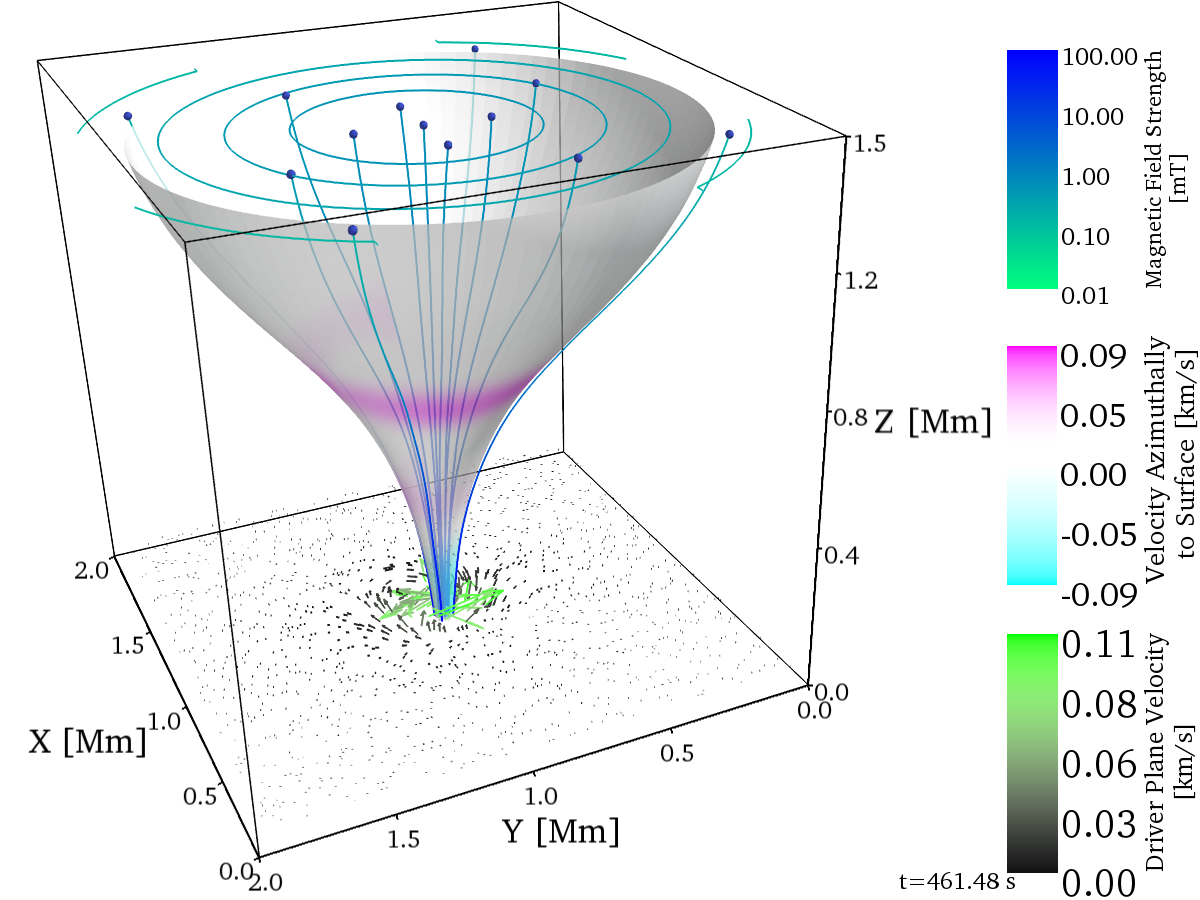
\includegraphics[width=0.55\columnwidth]{Chapter4/Figs/Mayavi_Slog_p240_A10_r60_vphi_00450.png}
        \caption{Snapshot at $t=461$ s}
    \end{subfigure}
    \begin{subfigure}[b]{0.9\columnwidth}
        \centering
        \includegraphics[width=0.55\columnwidth]{Chapter4/Figs/Mayavi_Slog_p240_A10_r60_vphi_00586.png}
        \caption{Snapshot at  $t=600$ s}
    \end{subfigure}
    \caption{Snapshots at three time steps of a 3D render of the simulation domain for the logarithmic spiral driver with a flux tube radius of $r = 936$ km (at the top of the computational domain). Shown in the domain are magnetic field lines and field strength contours in cyan, as well as the velocity vector field at the peak height of the driver shown as green and black arrows at the base, and the reconstructed surface coloured with the azimuthal velocity component ($V_\phi$).}
    \label{fig:frames_Suni_vphi}
\end{figure}

\subsection{Analysing Wave Excitation}\label{sec:driveranalysis}
The results of applying the analysis which is discussed in \cref{sec:fluxsurfaces} are shown in \cref{fig:frames_Suni_vphi}, as snapshots at times $154$, $461$ and $600 \text{ s}$ of wave propagation along the magnetic flux tube surface as generated by a logarithmic spiral driver with a period of $240$ s.
The strength and positions of these perturbations change as the simulations progress and the wave fronts travel along the tube. 
Also shown is a vector plane at the peak vertical height of the driver, which illustrates the velocity field driving the oscillations.
To analyse the propagation of separate wave modes we extracted the velocity components along a magnetic field line on the flux surface and constructed time-distance diagrams for each component. 
One magnetic field line is chosen at the beginning of the simulation and the values on the polygons between this field line and an adjacent field line are extracted for each time-step and presented in the time-distance diagrams in Fig. \ref{fig:All_TD_wave_30}. 
The perturbations are assumed to be linear, as no correction is made for the (vertical) movement of the surface itself. 
This assumption is verified by calculating the variation in the coordinates for the polygons at each time-step and it is found to be substantially less than one grid point for all the results presented here.

%In \cref{fig:All_TD_wave_30} it can be seen that the torsional driver excites perturbations in each velocity component, \textit{e.g.} $V_\phi$,  $V_\perp$, $V_\parallel$, as would be expected for a driver that is not exactly a linear eigenmode of the system. 

\subsubsection{Mode Identification}
To identify the observed MHD wave modes we shall initially consider the phase speed of the perturbations in the time-distance diagrams. 
In our numerical domain, both inside and outside the flux tube, the plasma $\beta > 1$.
To aid in the analysis of Fig. \ref{fig:All_TD_wave_30} overplotted are the Alfv\'en speed $v_A$ and sound speed $c_s$, as well as the speed of the fast magneto-acoustic wave (fast speed) $v_f^2 = \sqrt{c_s^2 + v_A^2}$ and the slow speed (or tube speed) $v_t^{-2} = \sqrt{c_s^{-2} + v_A^{-2}}$ for the equilibrium background, starting at $60$ s, the first peak of the driver amplitude. 
It should be noted that this analysis is still an approximation of our simulated system because we have non-constant, non-uniform, non-straight magnetic field in a stratified solar atmosphere, where one would expect the observed phase speed to deviate from these first-order estimations, as can be seen in Fig. \ref{fig:All_TD_wave_30}.

First, we take the case of the horizontal driver, Fig. \ref{fig:All_TD_wave_30:horiz}, in the most detail. 
In the $V_\parallel$ component we expect to see the fast sausage mode being the dominant mode, which is observed.
There is also a weaker presence of a perturbation with the phase speed closer to that of the Alfv\'en and slow speeds but offset from the starting point of the over-plotted lines; This is attributed to the coupling of the wave modes in our non-homogeneous plasma.
In the $V_\perp$ component the presence of a slow kink mode travelling close to the tube speed $v_t$ (solid line).
This mode is the dominant contribution in this panel and is approximately two times stronger when compared the perturbations in the parallel component. 
Finally, the azimuthal velocity component ($V_\phi$) has a very small contribution, of an order of magnitude less, travelling at the Alfv\'en speed, which we attribute to our driver not being perfectly centred upon the flux tube axis.

Comparing the results of the wave excitation by the vertical periodic driver to that of the horizontal driver, it is easy to draw parallels in the description.
However, there are some key differences. 
In this case, of wave excitation by the vertical driver, most of the perturbation is in the $V_\parallel$ velocity component, with a much stronger contribution from the fast sausage mode ($\approx 20 \times$ stronger than $V_\perp$).
There is also evidence of a rapidly spatially damped mode observed in the top panel of Fig. \ref{fig:All_TD_wave_30:vert}.
This spatial damping is attributed to the expansion of the magnetic flux tube, and the dispersion of the wave energy over a wider volume as the tube expands.
The $V_\perp$ component on the vertical driver's time-distance diagram is very weak, with only a weak fast kink mode component easily visible, apart from some small reflection from the top boundary. 
Finally, the vertical driver's $V_\phi$ component is, like its horizontally driven $V_\phi$ counterpart, substantially weaker than the other two components.

Next, we analyse the results of the three simulations with torsional drivers.
The time-distance diagrams for the three different torsional drivers have similar properties; the vast majority of the perturbation for all the torsional drivers is, as expected, in the $V_\phi$ component.
The other two components are of an order of magnitude less than the values of $V_\phi$.
The time-distance diagrams for the uniform torsional and the Archimedean spiral driver, Figs. \ref{fig:All_TD_wave_30:Suni} \& \ref{fig:All_TD_wave_30:Sarch}, have in their $V_\parallel$ component evidence of both the fast sausage mode travelling close to the fast speed, and another very weak mode travelling close to the slow speed.
We attribute this to the same wave mode coupling as observed in the horizontal driver's time-distance diagram. 
The logarithmic spiral simulation has a more predominant signature in the $V_\parallel$ velocity component, where the rapidly spatially damped slow sausage mode is the predominant signal, similar to that observed in the case of the vertical driver. 
In all three torsional drivers there is a notable presence of the coupled slow kink mode in the $V_\perp$ component. 


To gain a clearer understanding of the relative strength of each wave mode identified in Fig. \ref{fig:All_TD_wave_30} we now calculate the percentage wave energy flux carried by each component.

\begin{pycode}[chapter4]
import time_distance_plots as tdp

tube_r = 'r30'
drivers = ['horiz', 'vert', 'Suni', 'Sarch', 'Slog']
exp_facs = [None, None, 'B0', 'B0005', 'B005']
captions = ['Horizontal', 'Vertical', 'Circular', 'Archemedian Spiral', 'Logarithmic Spiral']

width = 0.49
figsize = list(texfigure.figsize(pytex, scale=width))
figsize[1] = 1.40*figsize[1]

v_td = texfigure.MultiFigure(3, 2, 'All_TD_wave_30')

for driver, exp_fac, caption in zip(drivers, exp_facs, captions):
    y, data, beta_line, all_times, all_spoints = tdp.get_data(ch4.data_dir, driver, tube_r, exp_fac)
    va_line, cs_line = tdp.get_speeds(ch4.data_dir, driver, tube_r, exp_fac)
    
    fig, axes = tdp.plot_paper1_td(data, all_times, y, beta_line, tube_r, figsize)
    tdp.overplot_speeds(axes, y, va_line, cs_line)
    plt.subplots_adjust(left=0.17,right=0.86,top=0.99,bottom=0.17)
    
    #fig.tight_layout(left=0.3,right=0.97,top=0.94,bottom=0.10)
    Fig = ch4.save_figure("All_TD_wave_30:{}".format(driver), fig, fext='.pdf')
    Fig.subfig_width = r'{}\columnwidth'.format(width)
    Fig.caption = '{} Driver'.format(caption)
    v_td.append(Fig)
    
v_td.caption = r"Decomposed velocity perturbation time-distance diagrams along the flux surface at radius $r = 468$ km for all simulated drivers. Horizontal black lines are plasma-$\beta$ contours, over-plotted are characteristic background speeds, the dot-dashed line is the fast speed ($v_f$), the dashed line is the sound speed ($c_s$), the dotted line is the Alfv\'en speed ($v_A$) and the solid line is the slow speed ($v_t$)."
\end{pycode}

\py[chapter4]|v_td|

%TODO: Wave Flux section needs rewriting
%Need to reference background section, and remove the avalible flux bullshit.
\subsection{Wave Energy Flux}\label{sec:energy_flux}

\begin{figure*}
    \centering
    \begin{subfigure}[b]{0.49\textwidth}
        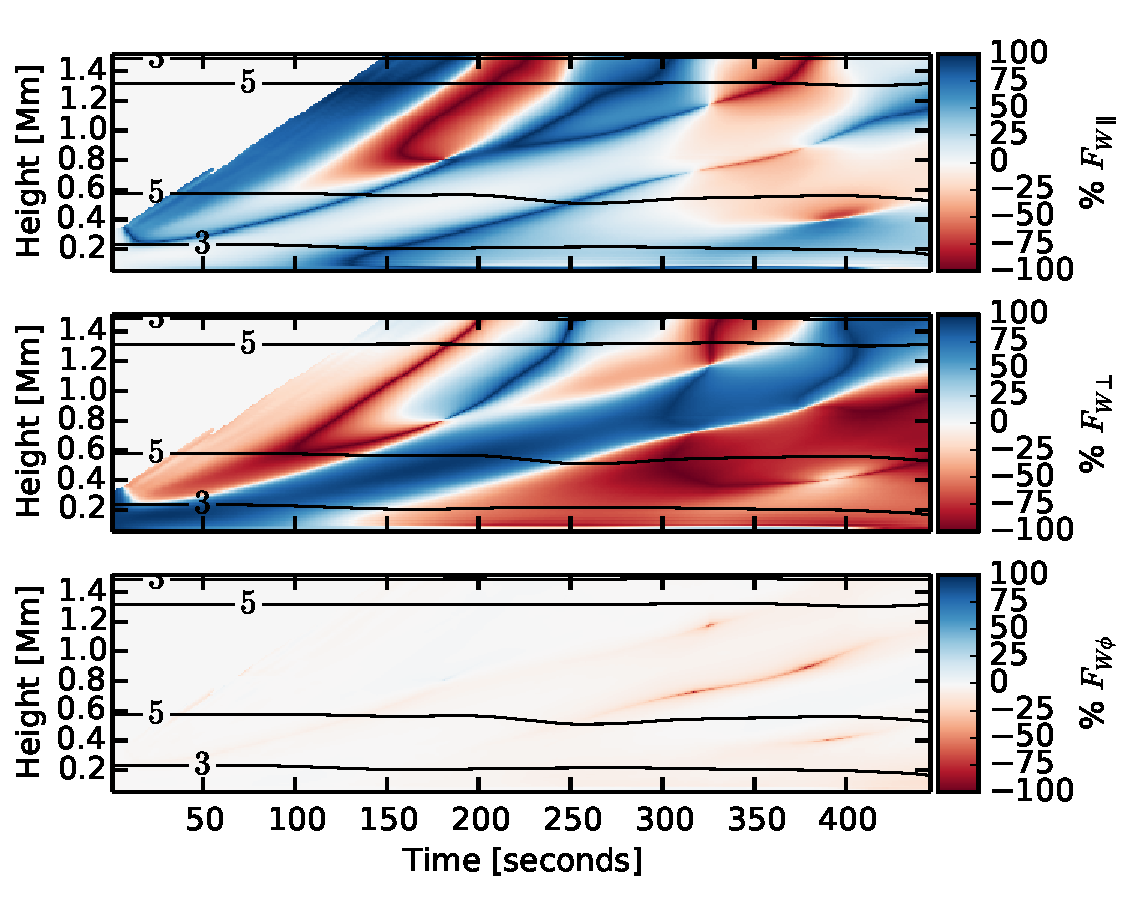
\includegraphics[width=\columnwidth]{Chapter4/Figs/WaveFlux_TD_Percent_horiz_p240_A10_r30.pdf}
        \caption{Horizontal Driver}
    \end{subfigure}
    \begin{subfigure}[b]{0.49\textwidth}
        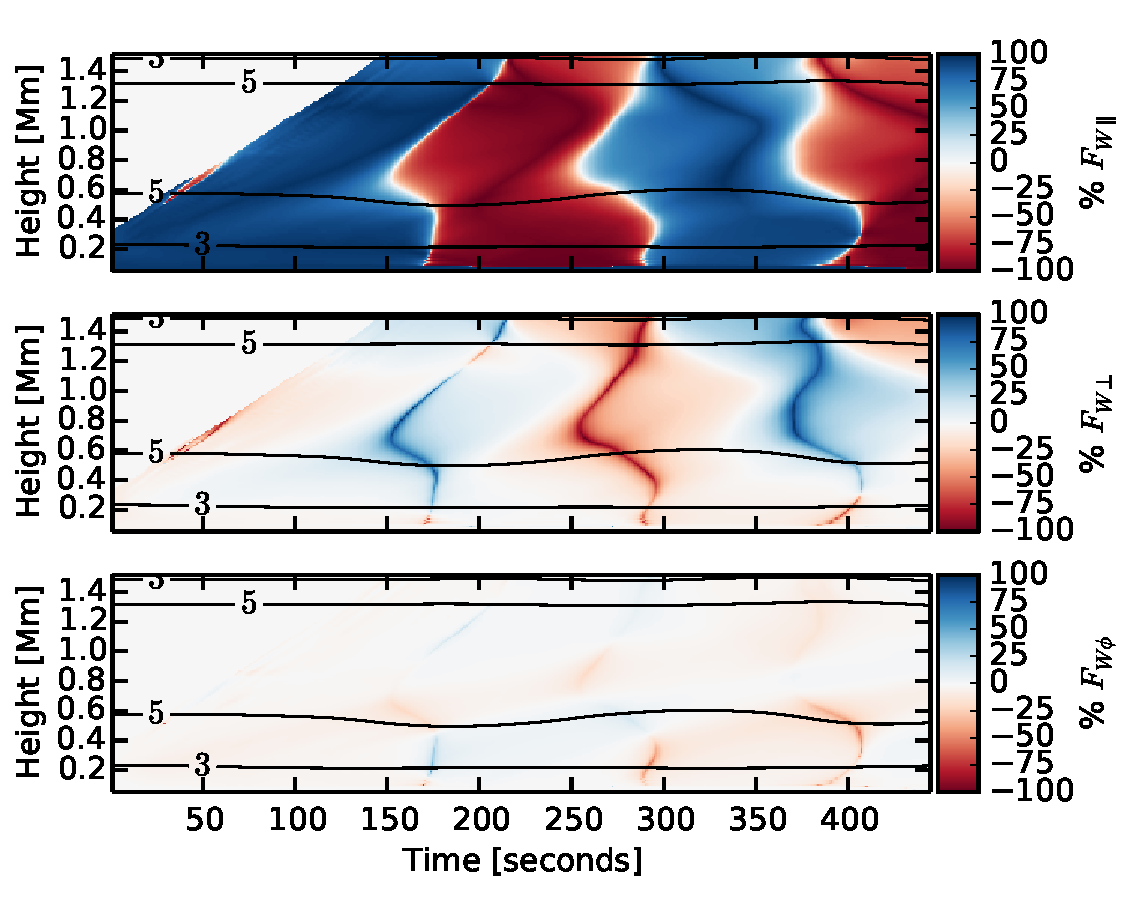
\includegraphics[width=\columnwidth]{Chapter4/Figs/WaveFlux_TD_Percent_vert_p240_A10_r30.pdf}
        \caption{Vertical Driver}
    \end{subfigure}
    
    \begin{subfigure}[b]{0.49\textwidth}
        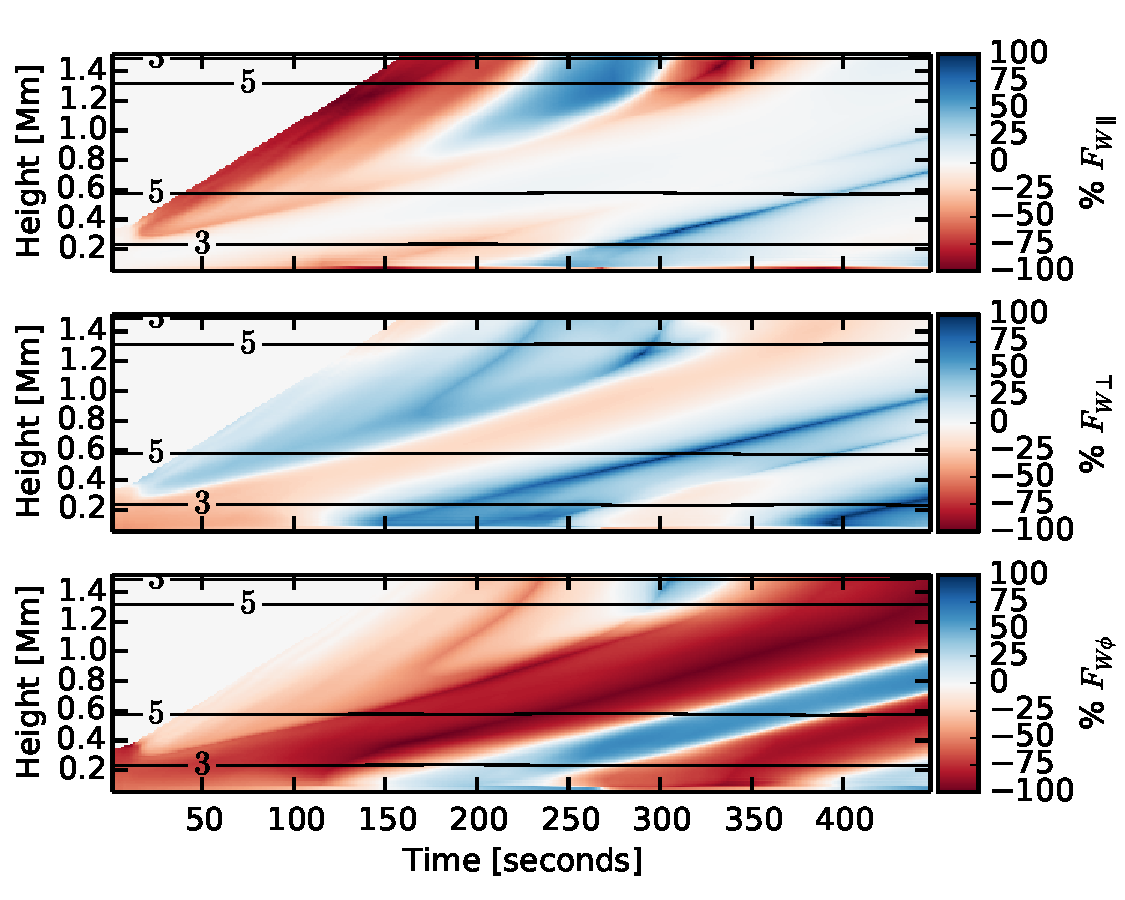
\includegraphics[width=\columnwidth]{Chapter4/Figs/WaveFlux_TD_Percent_Suni_p240_A10_r30_B0.pdf}
        \caption{Uniform Torsional Driver}
    \end{subfigure}
    \begin{subfigure}[b]{0.49\textwidth}
        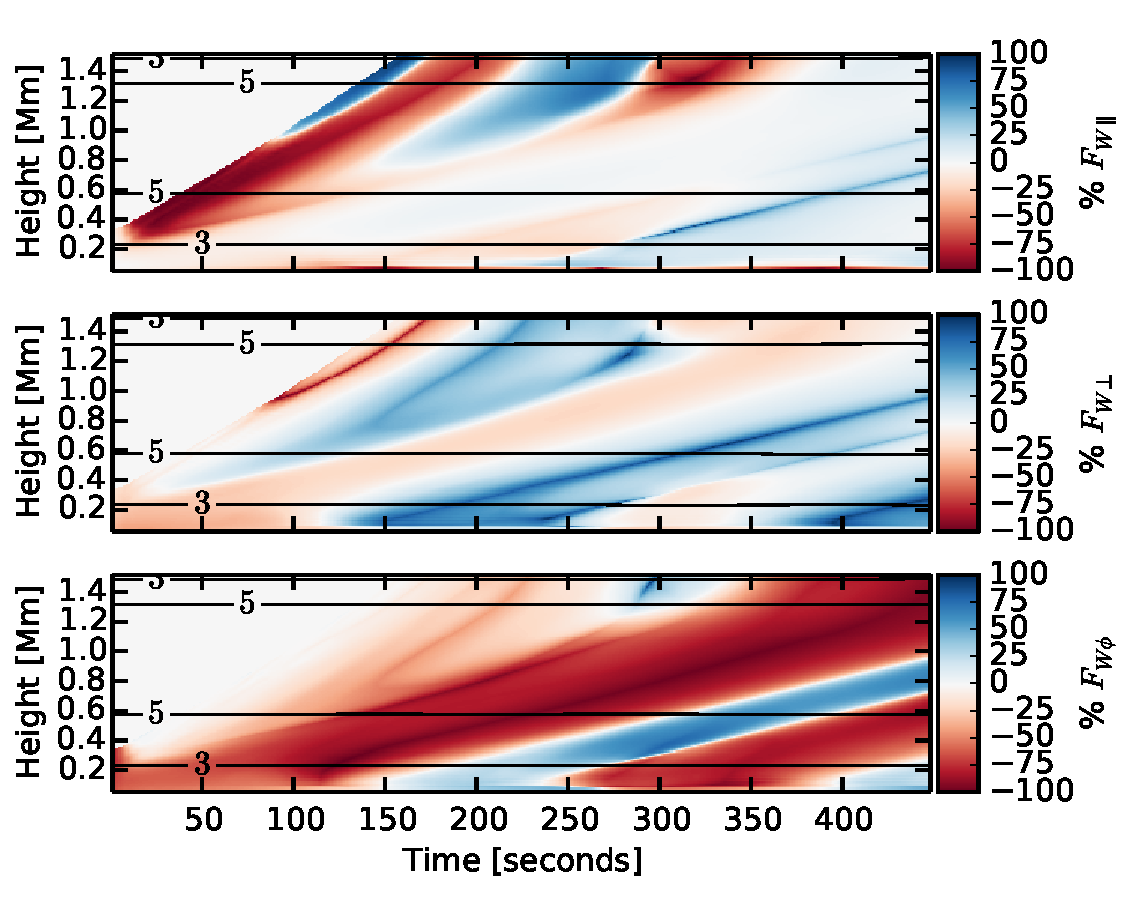
\includegraphics[width=\columnwidth]{Chapter4/Figs/WaveFlux_TD_Percent_Sarch_p240_A10_r30_B0005.pdf}
        \caption{Archimedean Spiral Type Driver}
    \end{subfigure}
    
    \begin{subfigure}[b]{0.49\textwidth}
        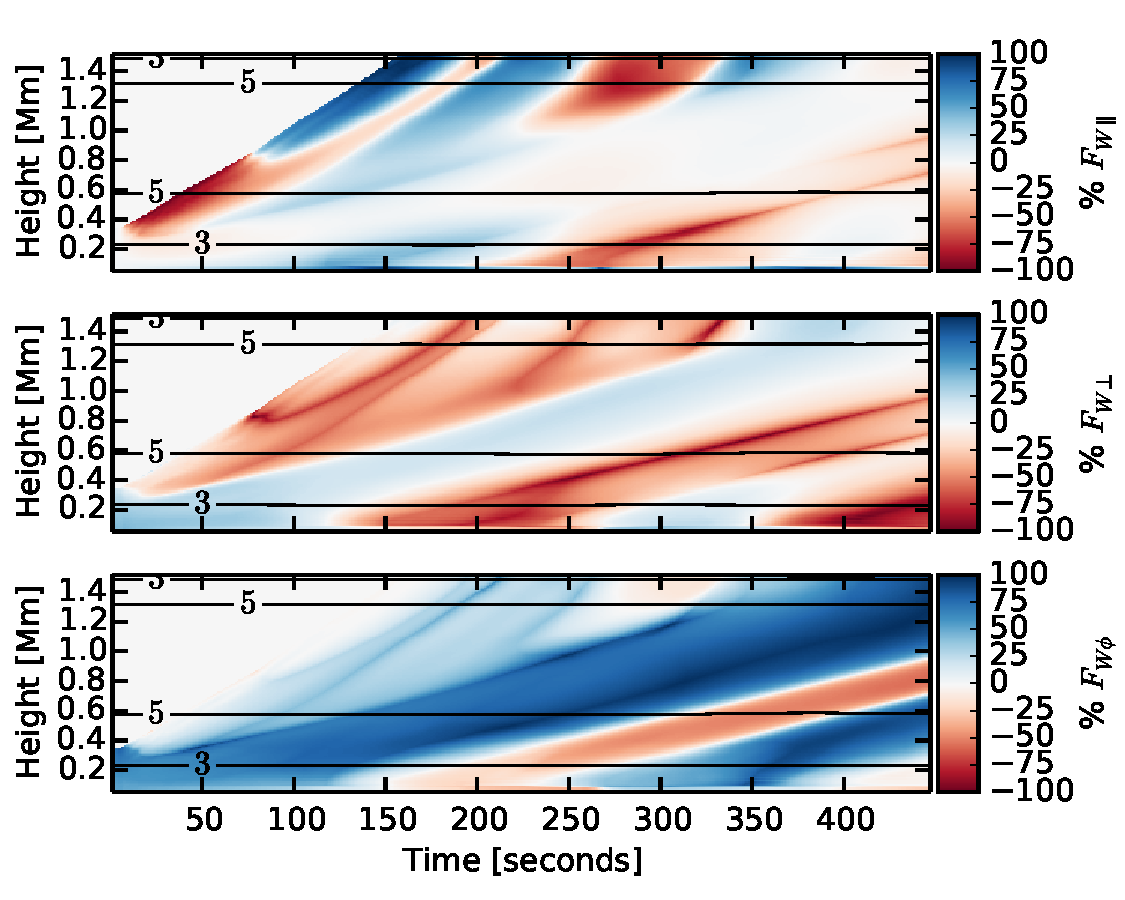
\includegraphics[width=\columnwidth]{Chapter4/Figs/WaveFlux_TD_Percent_Slog_p240_A10_r30_B005.pdf}
        \caption{Logarithmic Spiral Type Driver}
    \end{subfigure}
    \caption{Decomposed wave energy flux time-distance diagrams along the flux surface at radius $r = 468$ km (approximately central in the flux tube) for all simulated drivers. The three components of Energy flux ($F_\parallel$, $F_\perp$ and $F_\phi$) are calculated, then, the proportion for each component is shown for a strip up the flux surface.}
    \label{fig:All_Flux_percent_TD}
\end{figure*}

To calculate the relative strengths of the excited waves we compute the `wave energy flux' vector everywhere in the domain using Equation \ref{eq:wave_energy}.
\begin{equation}
\vec{F}_{wave} \equiv \widetilde{p}_k \vec{v} + \frac{1}{\mu_0} \left(\vec{B}_b \cdot \vec{\widetilde{B}}\right) \vec{v} - \frac{1}{\mu_0}\left(\vec{v} \cdot \vec{\widetilde{B}} \right) \vec{B}_b,
\label{eq:wave_energy2}
\end{equation}
where a subscript $b$ represents a background variable, a tilda represents a perturbation from the background conditions and $p_k$ represents kinetic pressure.

This equation has been widely used to calculate the energy contained in linear MHD perturbations.
It is discussed in detail in \cite{bogdan2003} where it is compared to the `true' MHD flux for linear perturbations and found to be generally clearer. 
It is used in \cite{vigeesh2009, vigeesh2012, khomenko2012}. 
For a full derivation and discussion relating to time-averaging see \cite{leroy1985}.
Calculating wave energy flux using Equation \ref{eq:wave_energy} provides a vector which is useful in plotting time distance diagrams and analysing wave modes.
Once the wave energy flux has been computed, it is decomposed into parallel, perpendicular and azimuthal components using the same method as the velocity vector. 
Using the analysis method outlined in Section \ref{sec:3d_analysis} time-distance diagrams are computed for the percentage wave energy flux (see Fig. \ref{fig:All_Flux_percent_TD}). 
The percentage values are plotted to highlight the relative strengths of the excited wave modes, and to enable a comparison of which modes are dominant. 
The absolute average energy flux over all heights is summed for all times for each component.


\begin{pycode}[chapter4]
#This is a direct yank of an old script

from flux_comparison import make_flux_bar_chart

fig = make_flux_bar_chart((texfigure.figsize(pytex)[0], 4.5), ch4.data_dir)
driver_flux = ch4.save_figure('flux-bar-graph', fig, fext='.pgf')
driver_flux.caption = r"Percentage total available energy flux comparison (calculated using Equations \ref{eq:flux_par} - \ref{eq:flux_phi}), for all drivers and all flux surfaces. The $F_\parallel$ component is shown as green, the $F_\perp$ component is shown in red and the $F_\phi$ component is shown in blue."
\end{pycode}

\py[chapter4]|driver_flux|


By comparing Figs. \ref{fig:All_TD_wave_30} \& \ref{fig:All_Flux_percent_TD} we find that for the wave modes excited by the horizontal driver $60$\% of the energy flux is in the perpendicular component $F_\perp$ which is attributed to the slow kink mode.
The rest of the flux is in the parallel component $F_\parallel$. 
The vertical driver simulation has $79.3$\% of the energy flux in the $F_\parallel$ component, identified as the fast sausage mode, with the $F_\perp$ component only contributing $12.5$\%. 
The simulations with spiral drivers all have up to $60$\% of their energy flux in the azimuthal component $F_\phi$. 
The logarithmic spiral source excites a slightly higher percentage of the flux in the slow kink mode and the fast sausage mode, in comparison to the uniform torsional and Archimedean spiral driver.

The summarised energy flux results, and their equivalents for different flux tube radii are shown in Fig. \ref{fig:flux_bar_graph}.
With reasonable accuracy we can attribute each of the energy flux components shown to one or two MHD wave modes.
The $F_\parallel$ component is generally the fast sausage mode. 
The $F_\perp$ component is almost exclusively excited by the slow kink mode.
Finally, the $F_\phi$ is attributed to the Alfv\'en mode.
Another interesting result is that the type of spiral driver used has a minimal impact upon the amount of flux in each wave mode (see Fig. \ref{fig:flux-bar-graph}).
This could be dependent upon the spiral expansion factor used in the logarithmic and Archimedean spirals, which could be the subject of a further parameter study.

\subsection{Flux Tube Radius}
The plasma properties vary within the computational domain due to the magnetic field configuration.
This also means that the wave propagation on the surface of a flux tube is dependent upon its radius. 
We define the radius of the flux tube at the top of the domain and as its initial radius.
There are an arbitrary number of definable flux tube surfaces in our domain as defined from the top outer edge of the domain inwards. 
To demonstrate the difference in propagation caused by the change in plasma properties, especially $\beta$, with a change in radii we have computed all the analysis for three different flux tubes, with radii of $r=936$ km, $r=468$ km and  $r=156$ km; These radii are chosen to represent a good spectrum across the domain.

The results of the flux calculations are summarised in Fig. \ref{fig:flux-bar-graph}.
The smallest radius flux tube, shown in the top panel, shows that, for the torsional driver simulations, less azimuthal ($F_\phi$) flux is generated closer to the axis of the flux tube. 
This is expected due to a higher magnetic pressure towards the axis of the tube; the flux is, instead, excited evenly in the parallel ($F_\parallel$) and perpendicular ($F_\perp$) components as predominately kink and sausage modes. 
For higher radii surfaces the $F_\parallel$ component dominates the $F_\perp$ component; as the distance from the axis increases the influence of the kink mode decreases.
In the case of the horizontal and vertical drivers, most of the flux is excited in the slow kink and sausage modes respectively.
In the horizontal case, for the larger radius tube, the sausage mode, in the $F_\parallel$ component, again begins to dominate the kink mode, in the $F_\perp$ component.

%*****************************************************************************************
%*********************************** Fith Chapter ****************************************
%*****************************************************************************************

\chapter{Effects of Expansion Factor on Logarithmic Spiral MHD Wave Excitation}

\begin{pycode}[chapter5]
ch5 = texfigure.Manager(pytex, number=5, base_path='./Chapter5/')

from streamlines import Streamlines

BL = np.array([0.015, 0.05, 0.15, 0.45, 1.5])

from sacconfig import SACConfig

cfg = SACConfig()
\end{pycode}

This work, as a follow-up to \cite{mumford2015}, investigates the effect of logarithmic spiral-type velocity drivers in the solar photosphere and their properties as MHD wave generation mechanisms.
\cite{mumford2015} studied five different photospheric velocity fields as drivers for MHD waves.
It was concluded that the logarithmic, Archemedian and uniform spiral drivers all generate similar ($\pm 10\%$) excited energy fluxes.
The spiral expansion factors were selected arbitrarily in \cite{mumford2015}.
This work analyses the effects of the spiral expansion factor on the MHD waves generated by these velocity fields, motivated by the observational studies and constraints of \cite{bonet2008}.
In \cite{bonet2008} magnetic bright points (MBPs) were observed spiralling in an inter-granular lane, where cold plasma sinks down into the convection zone.
\cite{bonet2008} fit the observed locations of the MBP with time to the equation for a logarithmic spiral, shown in Equation (\ref{eq:log_spiral}),
\begin{equation}
\theta = \frac{1}{B_L}\ln(r/a),
\label{eq:log_spiral}
\end{equation}
where $r$ is the radius of the spiral and $a$ is a positive real constant, and obtained a value of $B_L^{-1} = 6.4 \pm 1.6 = B_L = 0.15$ for the dimensionless expansion factor parameter.

In \cite{bonet2010} a larger sample of photospheric vortices were studied, despite not fitting spirals to the observed motions, a number density of photospheric vortices was calculated as $d \simeq 3.1 \times 10^{-3}$ vortices Mm$^{-2}$ minute$^{-1}$, which therefore provides an upper limit of the number of logarithmic spiral-like vortices in the solar photosphere.

In this work we investigate the role of the spiral expansion factor ($B_L$) in the generation of MHD waves in a non-potential Gaussian magnetic flux tube, embedded in a realistic stratified solar atmosphere.
The observational result of \cite{bonet2008} is used as a starting point and values $\pm 3\times$ and $\pm 10\times$ that value are then employed to give five points in the parameter space, centred around their result, which is illustrated in Figure \ref{fig:B_L_values}.


\section{Simulation Configuration}\label{sec:simconfig}
The simulations performed for this study utilise a realistic stratified solar atmosphere constructed by taking the VALIIIc \citep{vernazza1981} hydrodynamical properties and adding a non-potential self-similar magnetic field.
The self-similar magnetic field configuration is derived from the ones employed by \citet{fedun2011} and recently analytically described in \cite{gent2013, gent2014}; based on \citet{schluter1958, deinzer1965, low1980, schussler2005}, and identical to the one in \cite{mumford2015}.
A magnetic field is constructed via this method, then added to the hydrostatic background and then the pressure balance is satisfied using magneto-hydrostatic equilibrium as described by Equation~(\ref{eq:mhs-condition}), \textit{i.e.}
\begin{equation}
-(\mathbf{B_b}\cdot \nabla)\mathbf{B_b} + \nabla\left(\frac{\mathbf{B_b}^2}{2}\right) + \nabla p = \rho\mathbf{g}.
\label{eq:mhs-condition}
\end{equation}
(Equation~(\ref{eq:mhs-condition}) corrects the missing negative term in \cite{mumford2015}, the calculations are not affected.)
By using a magnetic foot point strength of $120$ mT and the background atmosphere as specified by the VALIIIc model, the resulting numerical domain has the plasma $\beta > 1$ at every point.

The Sheffield Advanced Code (SAC) \citep{Shelyag2008} used in this work is configured identically to \cite{mumford2015}. The domain has a spatial extent of $2.0 \times\ 2.0\ \times\ 1.6$ Mm$^3$, in $x$, $y$, $z$ respectively, with the origin in the $z$ direction $0.061$ Mm above the photosphere. The domain is divided up into $128^3$ grid points giving a physical size of $15.6\ \times\ 15.6\ \times\ 12.5$ km$^3$ for each grid cell.

The magnetohydrostatic background is perturbed during the simulations using a 3D Gaussian weighted logarithmic spiral velocity driver, as described by Equation~(\ref{eq: slog}) \citep{mumford2015}:
\begin{subequations}
    \begin{align}
    V_x &= A \frac{\cos(\theta + \phi)}{\sqrt{x^2 + y^2}}\ e^{-\left(\frac{z^2}{\Delta z^2} + \frac{x^2}{\Delta x^2} + \frac{y^2}{\Delta y^2}\right)} \sin \left(2\pi \frac{t}{P}\right),\\
    V_y &= - A \frac{\sin(\theta + \phi)}{\sqrt{x^2 + y^2}}\ e^{-\left(\frac{z^2}{\Delta z^2} + \frac{x^2}{\Delta x^2} + \frac{y^2}{\Delta y^2}\right)} \sin \left(2\pi \frac{t}{P}\right),\label{eq:Slog}\\
    \end{align}
    \label{eq: slog}
\end{subequations}
where:
\begin{equation*}
\theta = tan^{-1}\left(\frac{y}{x}\right),\ \phi = tan^{-1}\left(\frac{1}{B_L}\right),\notag	
\end{equation*}
$A=\frac{20}{\sqrt{3}}$, $\Delta x = \Delta y = 0.1$ Mm and $\Delta z = 0.05$ and $P=\py|int(cfg.period)|$ s.
Here, $B_L$ is the logarithmic spiral expansion factor discussed in Section~\ref{sec:intro}.

Figure \ref{fig:All_log_spirals} shows the calculated velocity profiles for the peak vertical height of the driver.
Overplotted on these profiles are streamlines that trace a logarithmic spiral with different expansion factors.

\begin{pycode}[chapter5]
size = list(texfigure.figsize(pytex))
size[1] = 1.5
fig, ax = plt.subplots(figsize=size)
ax.plot(BL, np.ones(BL.size), 'x', markersize=10, mew=2)
ax.errorbar([0.15], [1], xerr=np.array([[-1*(0.15-1/(6.4-1.6)), 0.15+1/(6.4+1.6)]]).T, mew=2, elinewidth=2)
ax.semilogx()
ax.get_yaxis().set_visible(False)
ax.set_frame_on(False)
ax.get_xaxis().tick_bottom()
ax.xaxis.set_tick_params(width=2)
ax.xaxis.set_tick_params(width=2, which='minor')
ax.xaxis.set_major_formatter(matplotlib.ticker.ScalarFormatter())
ax.xaxis.set_ticks(BL)
xmin, xmax, ymin, ymax = ax.axis()
ax.add_artist(plt.Line2D((xmin, xmax), (ymin, ymin), color='black', linewidth=1.4))
l = ax.set_xlim([0.01, 2.0])
l = ax.set_xlabel(r'$B_L$', fontsize=18)

fig.tight_layout(h_pad=0.01)
#bL_line = save_fig(cfg, fig=fig, fname='bline.pdf')

bL_line = ch5.save_figure('B_L_values', fig, fext='.pgf')
bL_line.caption = r"The parameter space of $B_L$ used in this work, with the $x$-axis on a logarithmic scale. The green error bars show the fit uncertainty of the value observed by \citet{bonet2008}."
\end{pycode}

\py[chapter5]|bL_line|

\begin{pycode}[chapter5]
#Use Equation 1 to calculate the vector field in a 2D plane to plot it.
time = np.linspace(0,60,480)
dt = time[1:] - time [:-1]
period = 240.

x = np.linspace(7812.5,1992187.5,128)
y = np.linspace(7812.5,1992187.5,128)

x_max = x.max()
y_max = y.max()

xc = 1.0e6
yc = 1.0e6

xn = x - xc
yn = y - yc

delta_x=0.1e6
delta_y=0.1e6

xx, yy = np.meshgrid(xn,yn)
exp_y = np.exp(-(yn**2.0/delta_y**2.0))
exp_x = np.exp(-(xn**2.0/delta_x**2.0))

exp_x2, exp_y2= np.meshgrid(exp_x,exp_y)
exp_xyz = exp_x2 * exp_y2


#==============================================================================
# Define Driver Equations and Parameters
#==============================================================================
#A is the amplitude, B is the spiral expansion factor
A = 1

#Tdamp defines the damping of the driver with time, Tdep is the ocillator
tdamp = lambda time1: 1.0 #*np.exp(-(time1/(period)))
tdep = lambda time1: np.sin((time1*2.0*np.pi)/period) * tdamp(time1)

#Define a peak index to use for scaling in the inital frame
max_ind = np.argmax(tdep(time) > 0.9998)

def get_log(B):
    #Logarithmic
    phi = np.arctan2(1,B)
    theta = np.arctan2(yy,xx)
    
    uy = np.sin(theta + phi)
    ux =  np.cos(theta + phi)
    
    vx = lambda time1: (ux / np.sqrt(ux**2 + uy**2)) * exp_xyz * tdep(time1) * A
    vy = lambda time1: (uy / np.sqrt(ux**2 + uy**2)) * exp_xyz * tdep(time1) * A
    
    vv = np.sqrt(vx(time[max_ind])**2 + vy(time[max_ind])**2)
    
    return vx, vy, vv

blfigs = texfigure.MultiFigure(3, 2, reference="All_log_spirals")
for bl in BL:
    fig, ax = plt.subplots(figsize=texfigure.figsize(pytex, 0.5),
                           gridspec_kw={'bottom':0.2, 'top':0.95})
    #============================================================================
    # Do the Plotting
    #============================================================================
    vx, vy, vv = get_log(bl)
    # Calculate Streamline
    slines = Streamlines(x,y,vx(time[max_ind]),vy(time[max_ind]),maxLen=7000,
    x0=xc, y0=yc, direction='forwards')
    
    im = ax.imshow(vv, cmap='Blues', extent=[7812.5,x_max,7812.5,y_max])
    im.set_norm(matplotlib.colors.Normalize(vmin=0,vmax=1))
    #ax.hold()
    
    Sline, = ax.plot(slines.streamlines[0][0],slines.streamlines[0][1],color='red',linewidth=2, zorder=40)
    
    #Add colourbar
    divider = make_axes_locatable(ax)
    cax = divider.append_axes("right", size="5%", pad=0.2)
    cbar = plt.colorbar(im,cax)
    cbar.set_label(r"$|V|$ [ms$^{-1}$]")
    scalar = matplotlib.ticker.ScalarFormatter(useMathText=False,useOffset=False)
    scalar.set_powerlimits((-3,3))
    cbar.formatter = scalar
    cbar.ax.yaxis.get_offset_text().set_visible(True)
    cbar.update_ticks()
    #cbar.solids.set_rasterized(True)
    cbar.solids.set_edgecolor("face")
    
    #Add quiver plot overlay
    #qu = ax.quiver(x,y,vx(time[max_ind]),vy(time[max_ind]),scale=25*A,color='k',zorder=20, linewidth=1)
    ax.axis([8.0e5,12.0e5,8.0e5,12.0e5])
    
    ax.xaxis.set_major_formatter(scalar)
    ax.yaxis.set_major_formatter(scalar)
    ax.xaxis.set_major_locator(matplotlib.ticker.MaxNLocator(5))
    ax.yaxis.set_major_locator(matplotlib.ticker.MaxNLocator(5))
    ax.xaxis.get_offset_text().set_visible(False)
    ax.yaxis.get_offset_text().set_visible(False)
    ax.set_xlabel("X [Mm]")
    ax.set_ylabel("Y [Mm]")
    
    #plt.tight_layout()
    
    Fig = ch5.save_figure('driver-{}'.format(bl).replace('.', '-'), fig)
    Fig.subfig_width = r'0.495\columnwidth'
    Fig.caption = r'$B_L = {}$'.format(bl)
    
    blfigs.append(Fig)
   
blfigs.caption = r"Cuts in the [$x$-$y$] plane through the driving velocity field. The magnitude of velocity is plotted in blue with velocity vectors overplotted in black and a streamline seeded at the centre plotted in red. A plot is shown for each value of $B_L$ used in a simulation."

\end{pycode}

\py[chapter5]|blfigs|

\section{Analysis}\label{sec:analysis}

To quantify the MHD wave modes generated by the logarithmic spiral velocity drivers it is necessary to quantify the relative proportion of the excited MHD wave modes.
The modes present in the domain are assumed to be uniquely determined by the three wave modes present in a uniform homogeneous plasma, namely, the fast magnetoacoustic mode, the slow magnetoacoustic mode and the Alfv\'en mode.
%TODO: WRONG WRONG WRONG
These three modes are separable into three vector components of perturbation with respect to the magnetic field.
The slow magnetoacoustic mode is the dominant contributor to the vector component perpendicular to the magnetic field vector.
The fast magnetoacoustic mode is the dominant mode in the parallel vector component with respect to the magnetic field.
The Alfv\'en mode can be identified in the third vector component found via the cross product of the parallel and perpendicular vector.
However, plasma geometry and conditions in the simulation domain make this approximation somewhat imperfect, because there are no clear MHD eigenmodes.
Further, these three modes become degenerate in cylindrical geometry giving rise to sausage, kink, and fluting modes.
Also, due to the complex plasma conditions in the simulation domain the modes may become physically coupled meaning that it is impossible to completely separate the modes.
Despite these complications the description of the modes based on the three vector components in the magnetic field frame is taken as a good way to describe, identify and quantify the MHD wave modes in the system.

To identify theses waves via the vector components relative to the magnetic field the identification of a vector perpendicular to the magnetic field vector is required.
In a 2D system this is a trivial step, however, in a 3D simulation it is ill-defined.
The solution to this problem, used in this work, is to define a magnetic flux surface which encapsulates a constant amount of magnetic flux at all heights in the domain.
This surface then allows the computation of a vector perpendicular to it and, thus, to the magnetic field lines it is constructed from.
These `flux surfaces' are initially constructed from a ring of axisymmetric field lines computed in the static background conditions.
The field line seed points then move with the plasma velocity throughout the simulation, which results in the flux surface being constructed from the same field lines at all times in the simulation.
The combination of the surface normal vectors and the magnetic field vector provide the information required to calculate the azimuthal vector via the cross product, which provides a third vector parallel to the surface but perpendicular to the magnetic field.

These surfaces are constructed, using the VTK library\footnote{Visualistation ToolKit 5.10.0 (\url{www.vtk.org})}, for three different characteristic initial radii (measured at the top of the domain) of $156$ km, $468$ km and $936$ km from the centre of the domain, for each simulation, giving a good sampling through the differing plasma properties of the domain.
This allows the analysis of the excited modes at different points in the domain, giving an overall picture of the waves.

Using the flux surfaces, defined above, we can now decompose any vector quantity in the domain into the parallel, perpendicular and azimuthal components, allowing study of the velocity and magnetic field perturbation vectors.
While the velocity and magnetic field perturbation vectors are good for identifying and studying wave behaviour itself, to quantify the amount of each wave mode generated the wave energy flux is computed using Equation (\ref{eq:wave_energy}) from \cite{bogdan2003}.

\begin{equation}
\vec{F}_{wave} \equiv \widetilde{p}_k \vec{v} + \frac{1}{\mu_0} \left(\vec{B}_b \cdot \vec{\widetilde{B}}\right) \vec{v} - \frac{1}{\mu_0}\left(\vec{v} \cdot \vec{\widetilde{B}} \right) \vec{B}_b,
\label{eq:wave_energy}
\end{equation}
where subscript $b$ represents a background variable, tilde represents a perturbation from the background conditions and $p_k$ represents kinetic pressure.

The wave energy flux (Equation (\ref{eq:wave_energy})) is decomposed onto the flux surface in the same way as the velocity vector, subject to the same limitations as the velocity.

\subsection{Results}\label{subsec:results}

To assist in the visualisation and analysis of the results provided by the flux surfaces the vector components along one field line are extracted for all time steps and plotted as time-distance diagrams in Figures \ref{fig:TD_velocity_r30} and \ref{fig:TD_flux_r30}.

Combining the decomposed velocity vector plotted in Figure \ref{fig:TD_velocity_r30} and the decomposed wave flux vector plotted in Figure \ref{fig:TD_flux_r30} we can reliably describe the nature of the waves generated in the simulations.
Overplotted on all panels in Figures~\ref{fig:TD_velocity_r30} \& \ref{fig:TD_flux_r30} are the phase speeds for the background conditions, the dot-dashed line is the fast speed $v_f$, the dashed line is the sound speed $c_s$, the dotted line is the Alfv\'en speed $v_A$ and the solid line is the slow speed $v_s$.
By comparing these characteristic wave mode speeds to the ridges in the time-distance diagrams it can be seen that in the panels for the torsional component (third panel in each figure), the dominant perturbation travels with the Alfv\'en speed (solid line).
We interpret this perturbation as an Alfv\'en wave.
For the perpendicular component (second panels) it can be seen that the dominant perturbation travels with the fast speed (dashed line), therefore this perturbation could be interpreted as a fast (kink or sausage) mode.
We can infer that this perturbation is more likely to be a sausage mode perturbation due to the nature of the driver, in that it should not perturb the axis of the flux tube and, that we observe no significant displacement on the flux surfaces during the simulation.
The most interesting result is shown for the parallel component (top panel in each figure), where for lower values of $B_L$, the amplitudes are low, but the perturbations that are present travel with the fast speed (dotted line).
However, as $B_L$ increases the perturbations change form.
There seems to appear a second, superimposed perturbation travelling with a speed close to that of the slow (or tube) speeds, which could be a slow sausage mode.
This second perturbation seems to grow proportionally to $B_L$, and can be seen to be dominant in Figures \ref{fig:TD_flux_r30_4} and \ref{fig:TD_flux_r30_5}.

The wave flux graphs in Figure \ref{fig:TD_flux_r30} are components normalised to the magnitude of the wave flux vector, thus showing the relative strengths of the components.
Taking Figure \ref{fig:TD_flux_r30_1} for the $B_L=\py|BL[0]|$ spiral it can be seen that most of the excited wave flux is in the azimuthal component, associated with the Alfv\'en wave.
As the expansion factor ($B_L$) increases, the driver becomes more radial, and the flux starts to shift from the azimuthal component into the parallel component.
This is interpreted as a change of the dominant mode from the torsional Alfv\'en wave into a sausage mode with dominant velocity perturbations parallel to the field lines.
Considering the range of $B_L$, found by \cite{bonet2008} and illustrated in the range spanned by Figure \ref{fig:TD_velocity_r30_3} and \ref{fig:TD_velocity_r30_4}, it can be seen that even within this parameter range the parallel component becomes substantially more dominant, meaning the change in spectrum of excited MHD wave modes is sensitive to the expansion factor of a spiral driver.

\cite{mumford2015} reported that there is a small but significant percentage of the wave energy flux contained in the perpendicular component.
This appears to be inversely coupled to the spiral expansion factor of the driver, as it decreases proportionally with the azimuthal wave flux component.
The size of the perpendicular component is also inversely proportional to the initial radius of the flux surface, as can be seen by its decrease in the three panels of Figure \ref{fig:flux_comparison}.

%\begin{pycode}[velTD]
%pflux_labels = {'par_label':r'$V_\parallel$ ms$^{-1}$', 
%'perp_label':r'$V_\perp$ ms$^{-1}$',
%'phi_label':r'$V_\phi$ ms$^{-1}$'}
%beta = False
%
%def add_triple_phase(ax, tube_r):
%ps = get_phase_speeds(cfg, tube_r)
%for ax0 in ax:
%add_phase_speeds(ax0, color='g', **ps)
%
%captions = []
%fnames = []
%for bl in BL:
%cfg.exp_fac = bl
%
%fig, ax = plt.subplots(nrows=3, ncols=1, figsize=(6,5))
%
%kwargs = get_single_velocity(cfg, 'r30', beta=beta)
%kwargs.update(pflux_labels)
%
%triple_plot(ax, **kwargs)
%
%#Remove the top two x labels
%ax[0].set_xlabel('')
%ax[1].set_xlabel('')
%add_triple_phase(ax, 'r30')
%#add_all_bpert(ax, 'r30')
%fig.tight_layout(h_pad=0.05)
%fnames.append(save_fig(cfg, fig=fig, fname='veltd_{}.pdf'.format(bl)))
%captions.append(r'$B_L = {}$'.format(bl))
%
%\end{pycode}
%
%\newcommand{\fwidth}{0.48\textwidth}
%\begin{figure*}
%    \centering
%    
%    \begin{subfigure}[b]{\fwidth}
%        \py[velTD]|get_pgf_include(fnames[0])|
%        \caption{\py[velTD]|captions[0]|}
%        \label{fig:TD_velocity_r30_1}
%    \end{subfigure}
%    \begin{subfigure}[b]{\fwidth}
%        \py[velTD]|get_pgf_include(fnames[1])|
%        \caption{\py[velTD]|captions[1]|}
%        \label{fig:TD_velocity_r30_2}
%    \end{subfigure}
%    
%    \begin{subfigure}[b]{\fwidth}
%        \py[velTD]|get_pgf_include(fnames[2])|
%        \caption{\py[velTD]|captions[2]|}
%        \label{fig:TD_velocity_r30_3}
%    \end{subfigure}
%    \begin{subfigure}[b]{\fwidth}
%        \py[velTD]|get_pgf_include(fnames[3])|
%        \caption{\py[velTD]|captions[3]|}
%        \label{fig:TD_velocity_r30_4}
%    \end{subfigure}
%    
%    \begin{subfigure}[b]{\fwidth}
%        \py[velTD]|get_pgf_include(fnames[4])|
%        \caption{\py[velTD]|captions[4]|}
%        \label{fig:TD_velocity_r30_5}
%    \end{subfigure}
%    \caption{
%        Velocity time-distance diagrams for all simulated values of $B_L$ for the surface with an initial top radius of $468$ km.
%        Shown in green are the phase speeds for the background conditions, the dot-dashed line is the fast speed $v_f$, the dashed line is the sound speed $c_s$, the dotted line is the Alfv\'en speed $v_A$ and the solid line is the slow speed $v_s$.
%        Note that plasma $\beta > 1$ for all heights in the domain.
%    }
%    \label{fig:TD_velocity_r30}
%\end{figure*}

%\begin{pycode}[fluxTD]
%pflux_labels = {'par_label':r'$F_\parallel / |\vec{F}|$ ms$^{-1}$', 
%'perp_label':r'$F_\perp / |\vec{F}|$ ms$^{-1}$',
%'phi_label':r'$F_\phi / |\vec{F}|$ ms$^{-1}$'}
%beta = False
%
%def add_triple_phase(ax, tube_r):
%ps = get_phase_speeds(cfg, tube_r)
%for ax0 in ax:
%add_phase_speeds(ax0, color='c', **ps)
%
%captions = []
%fnames = []
%for bl in BL:
%cfg.exp_fac = bl
%
%fig, ax = plt.subplots(nrows=3, ncols=1, figsize=(6,5))
%
%kwargs = get_single_percentage_flux(cfg, 'r30', beta=beta)
%kwargs.update(pflux_labels)
%kwargs.update({'cmap': 'PRGn'})
%
%triple_plot(ax, **kwargs)
%#Remove the top two x labels
%ax[0].set_xlabel('')
%ax[1].set_xlabel('')
%add_triple_phase(ax, 'r30')
%#add_all_bpert(ax, 'r30')
%fig.tight_layout(h_pad=0.05)
%fnames.append(save_fig(cfg, fig=fig, fname='fluxtd_{}.pdf'.format(bl)))
%pytex.fignum += 1
%captions.append(r'$B_L = {}$'.format(bl))
%
%\end{pycode}
%
%\begin{figure*}
%    \centering
%    
%    \begin{subfigure}[b]{\fwidth}
%        \py[fluxTD]|get_pgf_include(fnames[0])|
%        \caption{\py[fluxTD]|captions[0]|}
%        \label{fig:TD_flux_r30_1}
%    \end{subfigure}
%    \begin{subfigure}[b]{\fwidth}
%        \py[fluxTD]|get_pgf_include(fnames[1])|
%        \caption{\py[fluxTD]|captions[1]|}
%        \label{fig:TD_flux_r30_2}
%    \end{subfigure}
%    
%    \begin{subfigure}[b]{\fwidth}
%        \py[fluxTD]|get_pgf_include(fnames[2])|
%        \caption{\py[fluxTD]|captions[2]|}
%        \label{fig:TD_flux_r30_3}
%    \end{subfigure}
%    \begin{subfigure}[b]{\fwidth}
%        \py[fluxTD]|get_pgf_include(fnames[3])|
%        \caption{\py[fluxTD]|captions[3]|}
%        \label{fig:TD_flux_r30_4}
%    \end{subfigure}
%    
%    \begin{subfigure}[b]{\fwidth}
%        \py[fluxTD]|get_pgf_include(fnames[4])|
%        \caption{\py[fluxTD]|captions[4]|}
%        \label{fig:TD_flux_r30_5}
%    \end{subfigure}
%    \caption{
%        Normalised wave energy flux time-distance diagrams for all simulated values of $B_L$ for the surface with an initial top radius of $468$ km.
%        Shown in blue are the phase speeds for the background conditions, the dot-dashed line is the fast speed $v_f$, the dashed line is the sound speed $c_s$, the dotted line is the Alfv\'en speed $v_A$ and the solid line is the slow speed $v_s$.
%        Note that plasma $\beta > 1$ for all heights in the domain.
%    }
%    \label{fig:TD_flux_r30}
%\end{figure*}

This change in excitation of MHD waves is summarised in Figure \ref{fig:flux_comparison}, where the average value of $\displaystyle\frac{F_{\parallel, \perp, \phi}^2}{F_\parallel^2 + F_\perp^2 + F_\phi^2}$ for all time is plotted.
Figure \ref{fig:flux_comparison} shows that, between the values of $B_L=0.15$ and $B_L=0.45$ there is a turning point where the torsional component becomes less dominant, with expansion factors larger than $0.15$ having the parallel component being the dominant component.
This turning point occurs within the range of the fitted spirals in \cite{bonet2008} and, therefore, implies that photospheric spirals may indeed generate a variety of different MHD modes with varying strengths.
% !TeX root = ../smumford_thesis.tex
%*****************************************************************************************
%*********************************** Sixth Chapter ***************************************
%*****************************************************************************************
\begin{pycode}[chapter6]
from __future__ import print_function
ch6 = texfigure.Manager(pytex, number=6, base_path='./Chapter6/')

from sacconfig import SACConfig
cfg = SACConfig()
cfg.data_dir = ch6.data_dir

from streamlines import Streamlines
import td_plotting_helpers as ph

from period_amps import sim_params, periods
all_periods = sim_params[:10]
periods = periods[:10]
\end{pycode}

\chapter{Effects of Period on MHD Wave Generation from a Logarithmic Spiral Driver}\label{ch:period}

\Cref{ch:drivers,ch:expfac} studied the effects of the driving velocity profile and the logarithmic spiral expansion factor ($B_L$) on the MHD wave excitation.
In both of these previous chapters, arbitrary periods were chosen, in this chapter the effect of this choice of period on the wave excitation by the logarithmic driver is studied.
The solar photosphere is populated with an outstanding variety of different frequency wave modes.
Acoustic (p-mode) waves have a wide frequency spectra, with a peak power at 5 minutes, and a large number of MHD waves at different frequencies have been observed in the low solar atmosphere; \cite{Freij2014,Dorotovic2014} observe oscillations in magnetic pores at periods ranging from 3 minutes to 25 minutes; \cite{morton2011} observe sausage modes with periods ranging from $30$ to $447$ seconds; \cite{fujimura2009} observe oscillations with periods between $3$ and $6$ minutes in pores and between $4$ and $9$ minutes in the inter-granular lanes.
It is therefore interesting to study a range of possible frequencies for the driving motions, to see what effects this has on the excitation of MHD waves.

\section{Simulation Configuration}\label{sec:periodconfig}
This chapter employs the same magnetohydrostatic background as \cref{ch:drivers,ch:expfac} which is described in \cref{sec:mhsbackground}.
The plasma is also driven by the same logarithmic spiral driver as given in \cref{eq:Slog,eq:slog5}, the expansion factor is selected as the central point of the parameter sweep performed in \cref{ch:expfac}, \py[chapter6]|r"$B_L={}$".format(cfg.exp_fac)|.
A plot of the driver profile is shown in \cref{fig:slog-profile}.

\begin{pycode}[chapter6]

#Use Equation 1 to calculate the vector field in a 2D plane to plot it.
time = np.linspace(0,60,480)
dt = time[1:] - time [:-1]
period = 240.

x = np.linspace(7812.5,1992187.5,128)
y = np.linspace(7812.5,1992187.5,128)

x_max = x.max()
y_max = y.max()

xc = 1.0e6
yc = 1.0e6

xn = x - xc
yn = y - yc

delta_x=0.1e6
delta_y=0.1e6

xx, yy = np.meshgrid(xn,yn)
exp_y = np.exp(-(yn**2.0/delta_y**2.0))
exp_x = np.exp(-(xn**2.0/delta_x**2.0))

exp_x2, exp_y2= np.meshgrid(exp_x,exp_y)
exp_xyz = exp_x2 * exp_y2


#==============================================================================
# Define Driver Equations and Parameters
#==============================================================================
#A is the amplitude, B is the spiral expansion factor
A = 10

#Tdamp defines the damping of the driver with time, Tdep is the ocillator
tdamp = lambda time1: 1.0 #*np.exp(-(time1/(period)))
tdep = lambda time1: np.sin((time1*2.0*np.pi)/period) * tdamp(time1)

#Define a peak index to use for scaling in the inital frame
max_ind = np.argmax(tdep(time) > 0.9998)

#Logarithmic
B = 0.05
phi = np.arctan2(1,B)
theta = np.arctan2(yy,xx)

uy = np.sin(theta + phi)
ux =  np.cos(theta + phi)

vx = lambda time1: (ux / np.sqrt(ux**2 + uy**2)) * exp_xyz * tdep(time1) * A
vy = lambda time1: (uy / np.sqrt(ux**2 + uy**2)) * exp_xyz * tdep(time1) * A

vv = np.sqrt(vx(time[max_ind])**2 + vy(time[max_ind])**2)

# Calculate Streamline
slines = Streamlines(x,y,vx(time[max_ind]),vy(time[max_ind]),maxLen=7000,
x0=xc, y0=yc, direction='forwards')

#============================================================================
# Do the Plotting
#============================================================================

fig = plt.figure(figsize=texfigure.figsize(pytex))
ax = plt.subplot()
im = ax.imshow(vv, cmap='Blues', extent=[7812.5,x_max,7812.5,y_max])
im.set_norm(matplotlib.colors.Normalize(vmin=0,vmax=10))

Sline, = ax.plot(slines.streamlines[0][0],slines.streamlines[0][1],color='red',linewidth=2, zorder=40)

#Add colourbar
divider = make_axes_locatable(ax)
cax = divider.append_axes("right", size="5%", pad=0.2)
cbar = plt.colorbar(im,cax)
cbar.set_label(r"$|\vec{V}|$ [ms$^{-1}$]")
scalar = matplotlib.ticker.ScalarFormatter(useMathText=False,useOffset=False)
scalar.set_powerlimits((-3,3))
cbar.formatter = scalar
cbar.ax.yaxis.get_offset_text().set_visible(True)
cbar.update_ticks()
#cbar.solids.set_rasterized(True)
cbar.solids.set_edgecolor("face")

#Add quiver plot overlay
#qu = ax.quiver(x,y,vx(time[max_ind]),vy(time[max_ind]),scale=25*A,color='#00DDFF',zorder=20)
ax.axis([8.0e5,12.0e5,8.0e5,12.0e5])

ax.xaxis.set_major_formatter(scalar)
ax.yaxis.set_major_formatter(scalar)
ax.xaxis.set_major_locator(matplotlib.ticker.MaxNLocator(5))
ax.yaxis.set_major_locator(matplotlib.ticker.MaxNLocator(5))
ax.xaxis.get_offset_text().set_visible(False)
ax.yaxis.get_offset_text().set_visible(False)
ax.set_xlabel("X [Mm]")
ax.set_ylabel("Y [Mm]")

fig.tight_layout()

slog_fig = ch6.save_figure('slog-profile', fig=fig, fext='.pdf')
slog_fig.caption = r"Horizontal velocity profile of the logarithmic spiral driver with expansion factor $B_L = {}$. The magnitude of velocity is shown by the colour map and the cyan arrows follow the vector field. The red line is a velocity streamline seeded in the centre of the domain.".format(cfg.exp_fac)
slog_fig.figure_width=r'\columnwidth'
\end{pycode}

\py[chapter6]|slog_fig|

This chapter aims to vary the period ($P$) of the driver, and measure the effects on the wave excitation, however, varying the period of the driver will vary the total amount of energy added to the domain by the driver.
This would therefore heavily bias the analysis of the results, so it important that the amplitude of the driver is varied along with the period to maintain a constant energy input.
Below, the relationship between the period ($P$) and amplitude ($A$) is derived to maintain a constant amount of kinetic energy over the run time of the simulation ($T$) assuming $T = nP$, where $n$ is an integer.

The kinetic energy for any point in space at any instant in time is given by:
\begin{equation}
    E_k = \frac{1}{2}\ m\ v^2\label{eq:Ek}
\end{equation}
where $m$ is the mass and $v$ is the velocity.
Initially $E_T$ can be computed over an arbitrary volume $V$, which leads to:
\begin{equation}
    m = \rho(x,y,z)\ V.\label{eq:mass}
\end{equation}

The simulations are perturbed by a driver with the following general profile:
\begin{equation}
    v(x,y,z,t) = A\ G(x,y,z) \sin \left( \frac{2\pi t}{P} \right),\label{eq:vprofile}
\end{equation}
where $A$ is the amplitude of the velocity and $G(x,y,z)$ is a normalised spatial distribution.

Substituting \cref{eq:vprofile} into \cref{eq:Ek} for velocity gives:
\begin{align}
    E_{T}(x,y,z) &= \int_T \frac{1}{2}\ \rho(x,y,z)\ V\ A^2\ G^2(x,y,z)\ \sin^2\left(\frac{2\pi t}{P} \right) dt \\
    &= \frac{1}{2}\ \rho(x,y,z)\ V\ A^2\ G^2(x,y,z) \int_T \sin^2\left(\frac{2\pi t}{P} \right) dt \\
    & = \frac{1}{2}\ \rho(x,y,z)\ V\ A^2\ G^2(x,y,z) \left[ \frac{1}{2}T - \frac{P}{8\pi} \sin \left(\frac{4\pi T}{P} \right) \right]
\end{align}
recalling $T = nP$ this simplifies to 
\begin{equation}
    E_{T}(x,y,z) = \frac{nP}{4}\ \rho(x,y,z)\ V\ A^2\ G^2(x,y,z), \label{eq:Et_xyz}
\end{equation}

In the chosen background equilibrium the profile $\rho(x,y,z)$ is given by a numerical calculation from a reference background and modified for the presence of the magnetic flux tube.
This means that \cref{eq:Et_xyz} can only be numerically integrated and therefore, can be written as:
\begin{equation}
    E_T = \frac{nPA^2V}{4}\ \left( \sum_{x,y,z} \rho(x,y,z)\ G^2(x,y,z) \right),\label{eq:ET}
\end{equation}

\Cref{eq:ET} provides a relationship between the amplitude and period of the driver, however, it can be simplified by considering that many of the variables remain constant for each simulation performed in this chapter.
For all simulations run in this work the driver is the same, meaning $G(x,y,z)$ is constant, the background conditions and therefore $\rho(x,y,z)$ are also constant as is the numerical domain and therefore $V$.
It is therefore possible to let,
\begin{equation}
    Q = \frac{V}{4} \sum_{x,y,z} \rho(x,y,z)\ G^2(x,y,z)
\end{equation}
where $Q$ is a constant.
Substituting this into \cref{eq:ET} the final result is obtained:
\begin{align}
    E_T &= nPA^2\ Q, \\
    A^2 &= \frac{1}{E_T n Q} \frac{1}{P} \\
    A^2 &\propto \frac{1}{P}
\end{align}

Using the arbitrary amplitude selected in \cref{ch:drivers} of $10$ ms$^{-1}$, the desired amplitude for each of the periods selected can be calculated.
The result of this calculation is shown in \cref{tab:period-amp}.
\begin{table}
    \centering
    \begin{tabular}{cc}
        Period [seconds] & Amplitude [ms$^{-1}$] 	\\ \hline
        $30.0$           & $20\sqrt{2}$           	\\[2ex]
        $60.0$           & $20$  		            \\[2ex]
        $90.0$           & $20\sqrt{\frac{2}{3}}$  \\[2ex]
        $120.0$          & $10\sqrt{2}$        	\\[2ex]
        $150.0$          & $4\sqrt{10}$            \\[2ex]
        $180.0$          & $\frac{20}{\sqrt{3}}$   \\[2ex]
        $210.0$          & $20\sqrt{\frac{2}{7}}$  \\[2ex]
        $240.0$          & $10$                 	\\[2ex]
        $270.0$          & $\frac{20}{3}\sqrt{2}$  \\[2ex]
        $300.0$          & $4\sqrt{5}$           	\\[2ex]
        % $330.0$          & $20\sqrt{\frac{2}{11}}$ \\[2ex]
    \end{tabular}
    \caption{Tabulation of the period and amplitude pairs used in this work so that total kinetic energy input is constant.}
    \label{tab:period-amp}
\end{table}

\subsection{Results}\label{subsec:results}

To analyse the MHD wave generation we need to parametrise the relative strength of each component for different periods of driver.
To do this we decompose the velocity and the wave energy flux as defined in \cite{bogdan2003} onto the field line reference frame.
The velocity decomposition allows us to analyse the generated modes and identify what types of modes are in the generated spectra.
The wave energy flux analysis is presented in terms of $\vec{F}^2_j$ percentages, this allows a neat visualisation showing the relative strengths of each component, where the three components sum to $100\%$.


To make visualisation and analysis of the surfaces easier the values of the decomposed parameter is shown for one field line for all time steps in the simulation.
In Figure \ref{fig:TD-vel-r30} the values of velocity are shown in the form of time-distance diagrams for these field line strips, in Figure \ref{fig:TD-fwave-r30} the decomposed square wave flux is shown. Overlaid on both sets of plots are the characteristic phase speeds of a uniform plasma; the Alfv\'en speed $v_A$ and sound speed $c_s$, as well as the fast speed $v_f^2 = \sqrt{c_s^2 + v_A^2}$ and the slow (tube) speed $v_t^{-2} = \sqrt{c_s^{-2} + v_A^{-2}}$.
While these speeds will deviate from the true speeds in the non-uniform simulation domain, we can use them, in combination with knowledge of high-$\beta$ plasma properties to identify the wave modes present in the simulations.


It is clear from the $V_\phi$ (lowest) frames in Figure \ref{fig:TD-vel-r30} that the dominant perturbation is travelling at approximately the Alfv\'en speed, we can therefore reliably deduce that the torsional component of the velocity is, as expected, the Alfv\'en wave.
The $V_\perp$ (second) panels also a wave front propagating at the slow speed. For the high-$\beta$ plasma in the sub-chromosphere region of the solar atmosphere, this is the velocity component that is perturbed by the slow wave in a uniform plasma. In the shorter-period frames ($30$s and $90$s) there is a lower-amplitude front propagating close to the fast or sound speeds.
This is attributed to the coupling of the fast and slow wave modes due to the inhomogeneity of the plasma.
Finally, in the $V_\parallel$ (top) panels, there is not one dominant wave front, however evidence of two wave fronts, one propagating at the slow speed and one at the fast speed can be discerned.
The front propagating with the fast speed can be attributed to the fast mode, as in a uniform high-$\beta$ plasma the fast mode would perturb the parallel component of the velocity vector.
As with the $V_\perp$ component the existence of the slow mode is attributed to the non-uniform nature of the simulation domain.


The identification of the wave modes in the velocity perturbations can inform the analysis of the wave flux time-distance diagrams in Figure \
ref{fig:TD-fwave-r30}.
In Figure \ref{fig:TD-fwave-r30} the total square wave flux is calculated as the sum of the square of each component, $ F^2 = F_\parallel^2 + F_\perp ^2  + F_\phi^2$, the square of each component is then normalised by this square total to give a percentage value for each component.
This is then plotted along one field line, like the velocity components.


The percentage wave flux shown in Figure \ref{fig:TD-fwave-r30}, can be combined with the analysis of Figure \ref{fig:TD-vel-r30} to determine the relative strengths of the wave modes.
In comparison to the upper panels of Figure \ref{fig:TD-vel-r30}, where it was difficult to distinguish between the fronts travelling at the fast and slow speeds, in the $F^2_\parallel$ (top) panel of Figure \ref{fig:TD-fwave-r30} it is clear that the component with the most flux is the fast mode.
Figure \ref{fig:TD-fwave-r30} also shows that in the $F^2_\perp$ (middle) panel, the flux is more evenly shared between the two superimposed components, with the ratio apparently changing dependant upon period.
This observation should be considered when drawing conclusions from the relative strength of the $F^2_\parallel$ component.
The $F^2_\phi$ (bottom) panel is again dominated by the Alfv\'en component.

In Figure \ref{fig:period-flux} a summary of the average percentage square wave flux is presented for each of the \py[chapter6]|len(all_periods)| simulations performed.
The average value was taken for one field line for all time throughout the simulation.
The three panels of Figure \ref{fig:period-flux} are for three flux surfaces seeded at different initial radii at the top of the domain, showing results for different parts of the simulation domain.
In all three panels it can be seen that the averages for the perpendicular component (green dashes), remain constant with respect to period.
While the torsional (red crosses) and parallel (blue dots) components fluxes are clearly period dependant.
Recalling the analysis of Figures \ref{fig:TD-vel-r30} and \ref{fig:TD-fwave-r30} from above, we can attribute the perpendicular flux to the slow wave, the parallel flux to the fast wave and the torsional flux to the Alfv\'en wave.
We can therefore conclude that the relative strengths of the fast mode and the Alfv\'en mode are period dependant, with the Alfv\'en mode overall dominating more at larger periods.
While the growth in relative strength of the Alfv\'en mode is reasonably linear for the $156$ km radius flux surface, the larger flux surfaces show some variation in average wave flux. 


% SIX Velocity T-D Graphs:
\begin{pycode}[chapter6]

from period_amps import periods, str_amps
velocity_labels = {'par_label':r'$ \vec{V}_\parallel$ ms$^{-1}$', 
                   'perp_label':r'$ \vec{V}_\perp$ ms$^{-1}$',
                   'phi_label':r'$ \vec{V}_\phi$ ms$^{-1}$'}
beta = False
cfg.exp_fac = 0.15
ph.xxlim = 600

def add_all_bpert(ax, tube_r, N=4, levels=None):
    kwargs = ph.get_triple(cfg, beta=beta, single='bpert')
    x = kwargs['x_{}'.format(tube_r)]
    y = kwargs['y_{}'.format(tube_r)]
    par = kwargs['par_line_{}'.format(tube_r)].T[::-1, :]
    par[np.abs(par)<=1e-12] = 0
    perp = kwargs['perp_line_{}'.format(tube_r)].T[::-1, :]
    perp[np.abs(perp)<=1e-12] = 0
    phi = kwargs['phi_line_{}'.format(tube_r)].T[::-1, :]
    phi[np.abs(phi)<=1e-12] = 0
    ax[0].contour(x, y, par, N, colors='k', linewidths=np.linspace(0.5,1.5,N))
    ax[1].contour(x, y, perp, N, colors='k', linewidths=np.linspace(0.5,1.5,N))
    ax[2].contour(x, y, phi, N, colors='k', linewidths=np.linspace(0.5,1.5,N))	                   

def add_triple_phase(ax, tube_r):
    ps = ph.get_phase_speeds(cfg, tube_r)
    for ax0 in ax:
        ph.add_phase_speeds(ax0, color='g', **ps)

captions = {p: r"Period: ${}$ s Amplitude:".format(p) + a + r" ms$^{{-1}}$" for p, a in zip(periods, str_amps)[:10]}
#print(captions, file=sys.stderr)
width = 0.75
figsize = texfigure.figsize(pytex, scale=width, height_ratio=0.85)
multifig = texfigure.MultiFigure(len(all_periods), 1, reference='TD-vel-r30')
for i, paf in enumerate(all_periods):
    [setattr(cfg, f, getattr(paf, f)) for f in paf._fields]

    fig, ax = plt.subplots(nrows=3, ncols=1, figsize=figsize)
    
    kwargs = ph.get_single_velocity(cfg, 'r30', beta=beta)
    kwargs.update(velocity_labels)
    
    ph.triple_plot(ax, **kwargs)
    add_triple_phase(ax, 'r30')
    #Remove the top two x labels
    ax[0].set_xlabel('')
    ax[1].set_xlabel('')
    fig.tight_layout(h_pad=0.05)
    
    Lfig = ch6.save_figure('TD-vel-r30_p{}'.format(str(paf.period).replace('.','-')), fig=fig, fext='.pdf')
    Lfig.caption = "Velocity components for " + captions[paf.period]
    Lfig.subfig_width = r"{}\columnwidth".format(width)
    multifig.append(Lfig)

multifig.caption = r"""Velocity time-distance diagrams for six different period and amplitude combinations are plotted, in each pane three components of velocity are plotted for a flux surface of $r=468$ km. Overlaid on the velocity are magnetic field perturbation contours which are thicker for larger values and dashed for negative values. Shown in green are the phase speeds for the background conditions, the dot-dashed line is the fast speed $v_f$, the dashed line is the sound speed $c_s$, the dotted line is the Alfv\'en speed $v_a$ and the solid line is the slow speed $v_s$."""
\end{pycode}

\py[chapter6]|multifig[:2]|
\py[chapter6]|multifig[2:4]|
\py[chapter6]|multifig[4:6]|
\py[chapter6]|multifig[6:8]|
\py[chapter6]|multifig[8:10]|


\begin{pycode}[chapter6]
flux_labels = {'par_label':r'$F_\parallel^2$ \%', 
               'perp_label':r'$F_\perp^2$ \%',
               'phi_label':r'$F_\phi^2$ \%'}

multifig = texfigure.MultiFigure(len(all_periods), 1, reference='TD-fwave-r30')
for i, paf in enumerate(all_periods):
    [setattr(cfg, f, getattr(paf, f)) for f in paf._fields]
    
    fig, ax = plt.subplots(nrows=3, ncols=1, figsize=figsize)
    
    kwargs = ph.get_single_percentage_flux(cfg, 'r30', beta=beta)
    kwargs.update(flux_labels)
    kwargs.update({'cmap': 'PRGn'})
    ph.triple_plot(ax, **kwargs)
    add_triple_phase(ax, 'r30')
    #Remove the top two x labels
    ax[0].set_xlabel('')
    ax[1].set_xlabel('')
    fig.tight_layout(h_pad=0.05)
    
    Lfig = ch6.save_figure('TD_wave_r30_p{}'.format(str(paf.period).replace('.','-')), fig=fig, fext='.pdf')
    Lfig.caption = "Percentage $F^2$ components for " + captions[paf.period]
    Lfig.subfig_width = r"{}\columnwidth".format(width)
    multifig.append(Lfig)

multifig.caption = r"""Percentage square wave flux along one field line is plotted over the length of the simulation, for different period and amplitude combinations. Shown in green are the phase speeds for the background conditions, the dot-dashed line is the fast speed $v_f$, the dashed line is the sound speed $c_s$, the dotted line is the Alfv\'en speed $v_a$ and the solid line is the slow speed $v_s$."""

\end{pycode}


\py[chapter6]|multifig[:2]|
\py[chapter6]|multifig[2:4]|
\py[chapter6]|multifig[4:6]|
\py[chapter6]|multifig[6:8]|
\py[chapter6]|multifig[8:10]|


\begin{pycode}[chapter6]

from period_amps import periods, sim_params
sim_params = sim_params[:10]
periods = periods[:10]

size = texfigure.figsize(pytex, height_ratio=1.2)
fig, axs = plt.subplots(nrows=3, figsize=size, sharex=True)
titles = ["Flux Surface Radius $=156$ km", "Flux Surface Radius $=468$ km", "Flux Surface Radius $=936$ km"]
tubes = []
for i, ax in enumerate(axs):
    AvgsP = ph.get_all_avgs(cfg, cfg.tube_radii[i], sim_params)
    tubes.append(AvgsP)
    ax.plot(periods, AvgsP[0], 'o', label=r"$F_\parallel^2$", mew=0, ms=7)
    ax.plot(periods, AvgsP[1], '_', label=r"$F_\perp^2$", mew=2, ms=7)
    ax.plot(periods, AvgsP[2], 'x', label=r"$F_\phi^2$", mew=2, ms=7)
    ax.set_ylabel("% Square \n Wave Flux")
    ax.set_title(titles[i])
    ax.xaxis.set_major_formatter(matplotlib.ticker.ScalarFormatter())
    ax.xaxis.set_ticks(periods)
    ax.set_ylim([10, 75])
    ax.set_xlim([25, 305])

axs[-1].set_xlabel("Period [s]")

#axs[0].legend(bbox_to_anchor=(1.06, 1.05))
plt.tight_layout(h_pad=0.1)

period_flux = ch6.save_figure('period-flux', fig=fig, fext='.pgf')
period_flux.caption = r"""Average percentage square wave flux plotted against period. For each vector component on the flux surface the value of the wave flux squared along one field line is taken and then the fraction of the square total calculated, and then averaged over all time. This provides a high-level overview of the relative strengths of each mode. The azimuthal component is shown as red crosses, the parallel component as blue circles and the perpendicular component is shown as green dashes. The top panel displays the average wave flux for the flux surface closest to the centre of the domain at $r=156$ km the second panel at $r=468$ km and the bottom panel at $r=936$ km."""

\end{pycode}

\py[chapter6]|period_flux|

\section{Conclusion}\label{sec:conclusion}

In this chapter the same logarithmic spiral driver that was studied in \cref{ch:drivers,ch:expfac}, but varied the oscillatory period of the driver.



% !TeX root = ../smumford_thesis.tex
%*****************************************************************************************
%********************************** Seventh Chapter ***************************************
%*****************************************************************************************

\chapter{Conclusions and Future Work}\label{ch:conclusions}

\section{Summary and Conclusions}

This thesis has studied the generation of magnetohydrodynamic waves in the solar photosphere, and their propagation from the photosphere to the base of the chromosphere.
In \cref{ch:drivers}, five different photospheric drivers were used to excite MHD waves.
The vertical driver was found to excite primarily fast mode perturbations in the $V_\parallel$ component of the velocity.
The horizontal driver primarily excited slow mode perturbations in the perpendicular ($V_\perp$) component.
The three torsional drivers, a circular driver as well as Archemedian and logarithmic spirals all excited between $40$ and $60$ \% of their wave flux in the Alfv\'en mode, with the rest distributed between the fast and slow modes.
The uniformly low proportion of excited Alfv\'en wave for all the torsional drivers has an interesting implications for the generation of the widely sort after Alfv\'en wave.
If even idealised circular motions in the photosphere only excite $\approx 45$\% of their wave flux in the Alfv\'en mode, then the estimates of the total amount of available Alfv\'en flux, which could propagate through the chromosphere at potentially heat it and the corona, may be overestimated.

\Cref{ch:expfac} continued the study of the logarithmic spiral driver.
In this chapter, the expansion factor was varied and the effects on the distribution of excited wave modes studied.
In \cref{ch:drivers} the expansion factor was arbitrarily chosen to be $B_L = 0.05$, in \cref{ch:expfac} a variety of expansion factors were simulated based around the observational results of \cite{bonet2008}.
This study observed MBPs spiralling in a inter-granular lane, a logarithmic spiral was fitted to the observed locations of the MBP and a expansion factor of $B_L^{-1} = 6.4 \pm 1.6 = B_L = 0.15$ calculated.
Unlike the logarithmic spiral driver used in \cref{ch:drivers}, not all the expansion factors simulated in \cref{ch:expfac} resulted in the Alfv\'en wave being the dominant mode.
In fact, the midpoint of the parameter space studied, $B_L = 0.15$ was the last point simulated where the Alfv\'en mode was dominant, for the two points with higher expansion factors the fast mode was the dominant mode.
This accentuates the results of \cref{ch:drivers}, in that even less Alfv\'en flux is generated for driver profiles based on observational data.
If a distribution of expansion factors are present in the photosphere around the observed expansion factor $B_L = 0.15$ a large proportion of these vortexes would be generating more fast mode flux than Alfv\'en flux.

\Cref{ch:period} varied the driving period of the logarithmic spiral driver, while keeping the expansion factor at $B_L = 0.15$, in line with the simulations presented in \cref{ch:expfac}.
The period choices in \cref{ch:drivers,ch:expfac} were $240$ and $180$ s respectively, both of these were selected arbitrarily.
To cover a good range of the period parameter space, $10$ periods were selected varying from $30$ to $300$ seconds, in steps of $30$ s.
The upper limit of $300$ seconds being chosen for a combination of physical and practical purposes.
The maximum lifetime of the MBPs observed by \cite{sanchezalmeida2004} was $10$ minutes, so setting the upper limit as $300$ s allows for two complete periods with this upper bound of MBP lifetime.
In addition to this, running simulations for a much longer time period leads to interference by some reflection from the top numerical boundary.
The effects of the period on the excited wave mode distribution were varied.
The Alfv\'en fluxes varied up to a maximum of $20$\% for the narrowest flux surface, and substantially less than that for the other two wider surfaces.
Interestingly, however, there was some variation in the form of the observed wave fronts in the velocity time-distance diagrams.
At higher periods there is a small shift in the velocity perturbations from the fast mode to the slow mode ($V_\parallel$ to $V_\perp$).
This observation is not really reflected in the average wave flux results, however, there was a small increase in the perpendicular component for the last $3$ or $4$ periods in the sample.
Overall, it can be concluded that while the period has some effect on the wave modes generated, especially close to the axis of the flux tube, the effect is much less pronounced than for the other changes made to the driver in this thesis.

When considering the conclusion of this thesis, namely that spiral drivers excite a spectra of wave modes, it is worth keeping in mind the limitations of the analysis.
Primarily, the limitation of the spatial extent of the data studied.
Due to the need to construct flux surfaces to successfully decompose the vector quantities into a reference frame that lends itself to the analysis of MHD wave modes, these wave modes can, by definition, only be analysed on the constructed surfaces.
Throughout this thesis, three representative surfaces have been used to understand the dynamics at different points throughout the domain.
However, when considering the results, especially in \cref{ch:period}, where interesting results were observed close to the axis of the magnetic flux tube, it would be advantageous to be able to study the variation of the analysis continuously through the domain. 
In addition to this, the types of torsional oscillatory drivers used in these simulations have not been observed in the solar atmosphere.
The observations used for comparisons are of flows, presumed to be downward flows in inter-granular lanes, it would be an interesting extension of this work to study the effects of these downward spiral flows on wave excitation.

Beyond this fundamental limitation of the analysis method applied, the theoretical description of the plasma used to interpret the results presents some limitations.
Firstly, a uniform field approximation was described in \cref{ch:background}, this is an over-simplification of the numerical domain, where a plasma with some degree of spherical symmetry, in a stratified atmosphere was studied.
While much theory exists surrounding the nature of MHD waves in spherical geometry, this too would prove inadequate to analytically describe the plasma conditions in the simulation, indeed this is the purpose of numerical experiments.
However, some further analysis using this theory could be performed, especially utilising the spatial coordinates of the flux surfaces in the domain, to measure the displacement of the surface from the equilibria.

\section{Future Work}

The research documented in this thesis has explored a variety of parameters of the velocity fields that drive waves in the solar atmosphere.
The logarithmic spiral driver was studied the most intensely with the period and its expansion factor both analysed.
The scope for future work is vast, with substantially more parameters that could be varied.
One set of parameters which has remained constant over all the simulations run in this thesis is the FWHM of the Gaussian driving volume.
This parameter defines in what volume the majority  of the driving energy is added to the simulation.
In this thesis, this volume has been quite small, meaning most of the energy has been added close to the centre of the magnetic flux tube.
This may not be completely physical, because the plasma motions in the photosphere are not limited to the volume of a MBP, or even the inter-granular lane in which they are embedded.
When varying the FWHM of the driving profile it would be important to reconsider the analysis undertaken in \cref{ch:period} to ensure the total kinetic energy remained constant.
This would involve moving the $G(x,y,z)$ term out of the constant of proportionality, and accounting for it when selecting the amplitude.
The results of this study would be interesting, especially when analysing the difference between the flux surfaces closest to the centre of the magnetic flux tube, to the ones further away.

An effect that has not been explored in this thesis, is the effects of the boundary conditions on the results of the simulations.
Specifically, for the linear wave modes studied the magnetic field perturbations and the velocity pertubations should be tightly coupled.
This effect is not accounted for in the boundary conditions implemented by the SAC code, so the boundary conditions may introduce some coupling between the wave modes.
This effect and the coupling between the velocity and magnetic field could be investigated by driving the magnetic field as opposed to the velocity, as in an ideal plasma for linear waves the effects of this should be identical.

More fundamentally, the magnetic configuration itself could be varied.
With the work performed in \cite{gent2013,gent2014} it is trivial and computationally efficient to calculate multiple stable background atmospheres.
The atmosphere used in this work, is limited to below the transition region, because the expansion properties of the magnetic field, as used, would cause the pressure and density to become un-physical above this region.
Therefore, a different more self-consistent atmosphere should be built and the effects of the changing expansion rate on the wave generation studied.
If an atmosphere was constructed which had the same footpoint properties, \textit{e.g.} magnetic field strength and FWHM, the author hypothesises that the effects on the wave flux profiles would be minimal.
However, it is more than possible that the changes in plasma properties in the higher regions of the simulation domain would cause some deviation from the results presented in this thesis.

Finally, an interesting avenue for future study is to construct more complex background atmospheres from multiple flux tubes, such as in \cite{gent2014} and future extensions to that work.
This would allow for construction of an atmosphere based on observation data of the magnetic field, and more interestingly co-aligned observations of the photospheric velocity field.
While these results would more accurately mimic the reality of the solar surface they would present significant challenges in the analysis of the simulations.
The magnetic flux surface algorithm presented in \cref{sec:fluxsurfaces} is capable of selecting any flux surface even in a highly unstructured domain.
This would enable similar analysis to that of this thesis, however care would have to be taken in the interpretation.




% ********************************** Back Matter *******************************
% Backmatter should be commented out, if you are using appendices after References
%\backmatter

% ********************************** Bibliography ******************************
\begin{spacing}{0.9}

% To use the conventional natbib style referencing
% Bibliography style previews: http://nodonn.tipido.net/bibstyle.php
% Reference styles: http://sites.stat.psu.edu/~surajit/present/bib.htm

%\bibliographystyle{apalike}
\bibliographystyle{astron} % use this to have URLs listed in References
\cleardoublepage
\bibliography{References/Thesis} % Path to your References.bib file


% If you would like to use BibLaTeX for your references, pass `custombib' as
% an option in the document class. The location of 'reference.bib' should be
% specified in the preamble.tex file in the custombib section.
% Comment out the lines related to natbib above and uncomment the following line.

% \printbibliography[heading=bibintoc, title={References}]


\end{spacing}

% ********************************** Appendices ********************************

\begin{appendices} % Using appendices environment for more functunality

%% ******************************* Thesis Appendix A ********************************
\chapter{How to install \LaTeX} 

\section*{Windows OS}

\subsection*{TeXLive package - full version}
\begin{enumerate}
\item	Download the TeXLive ISO (2.2GB) from\\
\href{https://www.tug.org/texlive/}{https://www.tug.org/texlive/}
\item	Download WinCDEmu (if you don't have a virtual drive) from \\
\href{http://wincdemu.sysprogs.org/download/}{http://wincdemu.sysprogs.org/download/}
\item	To install Windows CD Emulator follow the instructions at\\
\href{http://wincdemu.sysprogs.org/tutorials/install/}{http://wincdemu.sysprogs.org/tutorials/install/}
\item	Right click the iso and mount it using the WinCDEmu as shown in \\
\href{http://wincdemu.sysprogs.org/tutorials/mount/}{http://wincdemu.sysprogs.org/tutorials/mount/}
\item	Open your virtual drive and run setup.pl
\end{enumerate}

or

\subsection*{Basic MikTeX - \TeX~ distribution}
\begin{enumerate}
\item	Download Basic-MiK\TeX (32bit or 64bit) from\\
\href{http://miktex.org/download}{http://miktex.org/download}
\item	Run the installer 
\item	To add a new package go to Start >> All Programs >> MikTex >> Maintenance (Admin) and choose Package Manager
\item	Select or search for packages to install
\end{enumerate}

\subsection*{TexStudio - \TeX~ editor}
\begin{enumerate}
\item	Download TexStudio from\\
\href{http://texstudio.sourceforge.net/\#downloads}{http://texstudio.sourceforge.net/\#downloads} 
\item	Run the installer
\end{enumerate}

\section*{Mac OS X}
\subsection*{MacTeX - \TeX~ distribution}
\begin{enumerate}
\item	Download the file from\\
\href{https://www.tug.org/mactex/}{https://www.tug.org/mactex/}
\item	Extract and double click to run the installer. It does the entire configuration, sit back and relax.
\end{enumerate}

\subsection*{TexStudio - \TeX~ editor}
\begin{enumerate}
\item	Download TexStudio from\\
\href{http://texstudio.sourceforge.net/\#downloads}{http://texstudio.sourceforge.net/\#downloads} 
\item	Extract and Start
\end{enumerate}


\section*{Unix/Linux}
\subsection*{TeXLive - \TeX~ distribution}
\subsubsection*{Getting the distribution:}
\begin{enumerate}
\item	TexLive can be downloaded from\\
\href{http://www.tug.org/texlive/acquire-netinstall.html}{http://www.tug.org/texlive/acquire-netinstall.html}.
\item	TexLive is provided by most operating system you can use (rpm,apt-get or yum) to get TexLive distributions
\end{enumerate}

\subsubsection*{Installation}
\begin{enumerate}
\item	Mount the ISO file in the mnt directory
\begin{verbatim}
mount -t iso9660 -o ro,loop,noauto /your/texlive####.iso /mnt
\end{verbatim}

\item	Install wget on your OS (use rpm, apt-get or yum install)
\item	Run the installer script install-tl.
\begin{verbatim}
	cd /your/download/directory
	./install-tl
\end{verbatim}
\item	Enter command `i' for installation

\item	Post-Installation configuration:\\
\href{http://www.tug.org/texlive/doc/texlive-en/texlive-en.html\#x1-320003.4.1}{http://www.tug.org/texlive/doc/texlive-en/texlive-en.html\#x1-320003.4.1} 
\item	Set the path for the directory of TexLive binaries in your .bashrc file
\end{enumerate}

\subsubsection*{For 32bit OS}
For Bourne-compatible shells such as bash, and using Intel x86 GNU/Linux and a default directory setup as an example, the file to edit might be \begin{verbatim}
edit $~/.bashrc file and add following lines
PATH=/usr/local/texlive/2011/bin/i386-linux:$PATH; 
export PATH 
MANPATH=/usr/local/texlive/2011/texmf/doc/man:$MANPATH;
export MANPATH 
INFOPATH=/usr/local/texlive/2011/texmf/doc/info:$INFOPATH;
export INFOPATH
\end{verbatim}
\subsubsection*{For 64bit OS}
\begin{verbatim}
edit $~/.bashrc file and add following lines
PATH=/usr/local/texlive/2011/bin/x86_64-linux:$PATH;
export PATH 
MANPATH=/usr/local/texlive/2011/texmf/doc/man:$MANPATH;
export MANPATH 
INFOPATH=/usr/local/texlive/2011/texmf/doc/info:$INFOPATH;
export INFOPATH

\end{verbatim}



%\subsection{Installing directly using Linux packages} 
\subsubsection*{Fedora/RedHat/CentOS:}
\begin{verbatim} 
sudo yum install texlive 
sudo yum install psutils 
\end{verbatim}


\subsubsection*{SUSE:}
\begin{verbatim}
sudo zypper install texlive
\end{verbatim}


\subsubsection*{Debian/Ubuntu:}
\begin{verbatim} 
sudo apt-get install texlive texlive-latex-extra 
sudo apt-get install psutils
\end{verbatim}


\end{appendices}

% *************************************** Index ********************************
\printthesisindex % If index is present

\end{document}
